% Created 2024-09-07 sá. 16:33
% Intended LaTeX compiler: pdflatex
\documentclass[oldfontcommands, a4paper, 11pt]{memoir}
\usepackage{color}
\usepackage{listings}
\aliaspagestyle{title}{empty}
\aliaspagestyle{part}{empty}
%estilo de capitulos
\chapterstyle{veelo} %  This style created by Bastiaan Veelo and is raggedleft, large, bold and with a black square in the margin by the number line.
%\chapterstyle{ger} % This style was created by Gerardo Garcia8 and is a two line, raggedright, large bold style with rules above and below.

%Idioma español y acentos
\usepackage[spanish]{babel}
%\usepackage[latin1]{inputenc}
\usepackage[utf8]{inputenc}

%algunos sÌmbolos matemáticos y paquetes para usar subimágenes
\usepackage{amsmath}
\usepackage{amsfonts}
\usepackage{amssymb}
\usepackage{graphicx}
\usepackage{appendix}
%Márgenes
\usepackage[left=3cm,top=3cm,right=3cm,bottom=3cm]{geometry}

%multi columnas
\usepackage{multicol}

%colores
\usepackage[dvipsnames]{xcolor}

%código
\usepackage{verbatim}

%para generar índice con hipervínculos
\usepackage{hyperref}
\hypersetup{
    colorlinks=true,       % false: boxed links; true: colored links
    linkcolor=Brown,          % color of internal links
    citecolor=BrickRed,        % color of links to bibliography
    filecolor=black,      % color of file links
    urlcolor=Blue           % color of external links 
}

%nomenclatura
\usepackage{nomencl}
\makenomenclature

%traducciones
\addto\captionsspanish{%
	\def\tablename{Tabla}%
	\def\listtablename{\'Indice de tablas}}

\renewcommand\nomname{Nomenclatura}
\def\nompreamble{\addcontentsline{toc}{chapter}{\nomname}\markboth{\nomname}{\nomname}}

%configuración de listings
% \lstset{
%   language=R,
%   numberstyle=\tiny\color{Blue},
%   framexleftmargin=5mm,
%   xleftmargin=\parindent,
%   keywordstyle=\color{Blue},
%   emphstyle=\color{Blue},
%   commentstyle=\color{YellowGreen},
%   stringstyle=\color{YellowOrange},
%   basicstyle=\ttfamily\small,
%   index=[1][emph],
%   indexstyle=[1]\indexfunctions,
%   columns=fullflexible,
%   breaklines=true,
%   linewidth=\textwidth,
%   backgroundcolor=\color{gray!7},
%   basewidth={0.5em,0.4em},
%   showstringspaces=false,
%   frame=single,
%   literate={á}{{\'a}}1 {ñ}{{\~n}}1 {é}{{\'e}}1 {ó}{{\'o}}1 {º}{{\textordmasculine}}1
%   }

\definecolor{mediumgray}{rgb}{0.3, 0.4, 0.4}
\definecolor{mediumblue}{rgb}{0.16, 0.5, 0.73}
\definecolor{forestgreen}{rgb}{0.13, 0.55, 0.13}
\definecolor{darkviolet}{rgb}{0.58, 0.0, 0.83}
\definecolor{royalblue}{rgb}{0.25, 0.41, 0.88}
\definecolor{crimson}{rgb}{0.86, 0.8, 0.24}
\definecolor{lightgrey}{rgb}{0.97, 0.97, 0.97}
\definecolor{black}{rgb}{0.05, 0.05, 0.1}
\definecolor{green}{rgb}{0.1529, 0.6823, 0.3764}
\definecolor{red6}{rgb}{0.753, 0.224, 0.169}

\lstset{
  language = R,
  backgroundcolor=\color{lightgrey},
  basicstyle=\fontsize{10}{12}\selectfont\ttfamily,
  breakatwhitespace=false,
  breaklines=false,
  captionpos=b,
  columns=fullflexible,
  commentstyle=\color{mediumgray}\upshape,
  emph={},
  emphstyle=\color{crimson},
  extendedchars=true,  % requires inputenc
  fontadjust=true,
  frame=single,
  identifierstyle=\color{black},
  keepspaces=true,
  keywordstyle=\color{mediumblue},
  keywordstyle={[2]\color{darkviolet}},
  keywordstyle={[3]\color{red}},
  numbers=left,
  numbersep=10pt,
  numberstyle=\tiny\color{black},
  rulecolor=\color{black},
  showlines=true,
  showspaces=false,
  showstringspaces=false,
  showtabs=false,
  stringstyle=\color{green},
  tabsize=2,
  title=\lstname,
  upquote=true  % requires textcomp
}


%configuración de verbatim
\usepackage{fancyvrb}
\DefineVerbatimEnvironment{verbatim}{Verbatim}{
  fontsize=\fontsize{8}{8},
  formatcom = {\color{black!70}}}

%bibliografia
% \usepackage[citestyle=authoryear,bibstyle=authoryear,doi=true,url=true]{biblatex}
% \let\cite\parencite
\usepackage[backend=biber, style=alphabetic, sorting=ynt]{biblatex}
\addbibresource{bibliografia/bibliografia.bib}



\author{Francisco Delgado López}
\date{\today}
\title{Francisco Delgado López - Desarrollo de una herramienta software para la simulación de sistemas fotovoltaicos con R - 2024}
\hypersetup{
 pdfauthor={Francisco Delgado López},
 pdftitle={Francisco Delgado López - Desarrollo de una herramienta software para la simulación de sistemas fotovoltaicos con R - 2024},
 pdfkeywords={geometría solar, radiación solar, energía solar, fotovoltaica, métodos de visualización, series temporales, datos espacio-temporales, S4},
 pdfsubject={Desarrollo de una herramienta software para la simulación de sistemas fotovoltaicos con R - 2024},
 pdfcreator={Emacs 29.2 (Org mode 9.6.15)}, 
 pdflang={Spanish}}
\begin{document}

\frontmatter

\begin{center}
\thispagestyle{empty}

\includegraphics[scale=1]{figuras/cabecera.pdf}\\
\vspace*{1cm}
\Large{\textbf{\MakeUppercase{Universidad Politécnica de Madrid}}}\\[3mm]
\Large{{\MakeUppercase{Escuela técnica superior de ingeniería y diseño industrial}}}\\[3mm]
\Large {Grado en Ingeniería Eléctrica}\\
\vfill
\line(1,0){400}\\
\Large{{\MakeUppercase{Trabajo de fin de grado}}}\\
\Huge{\textbf{Título}}\\[5mm]
\Large{Autor: Francisco Delgado López}\\
\line(1,0){400}\\
\vfill
\end{center}
\begin{flushright}
\Large {Tutor: Oscar Perpiñán Lamigueiro}\\[3mm]
\Large{Departamento de Ingeniería Eléctrica,\\ Electrónica, Automática y Física aplicada}\\[10mm]
Madrid, \today
\end{flushright}
\cleardoublepage 


\chapter{Agradecimientos}

Agradezco a ............



\chapter{Resumen}

Este proyecto se resume en \ldots{}\ldots{}\ldots{}\ldots{}\ldots{}

\section*{Palabras clave}
palabraclave1, palabraclave2, palabraclave3

\chapter{Abstract}

In this project\ldots{}\ldots{}\ldots{}

\section*{Keywords:}
keyword1, keyword2, keyword3

\cleardoublepage

\tableofcontents
\cleardoublepage

\listoffigures
\cleardoublepage

\printnomenclature{}
\cleardoublepage


\mainmatter

\chapter{Introducción}
\label{chap:introduccion}

\section{Objetivos}
\label{sec:orga469e6d}
\label{sec:objetivos}
El objetivo principal de este proyecto es el desarrollo de un paquete en R \cite{rcoreteam23} con el cual poder realizar estimaciones y representaciones gráficas de la geometría solar, radiación solar en el plano horizontal y del generador, y el funcionamiento de sistemas fotovoltaicos de conexión a red y de bombeo de agua.

Durante el resto del documento, si fuera necesario, se hará referencia al paquete desarrollado en este proyecto con el nombre \href{https://solarization.github.io/solaR2/}{solaR2}.

El usuario puede colocar los datos que considere convenientes (desde una base de datos oficial, una base de datos propia\ldots{} etc.) en cada una de las funciones que ofrece el paquete pudiendo así obtener resultados de la geometría solar, de la radiación horizontal, de la efectiva y hasta de la producción de diferentes tipos de sistemas fotovoltaicos.

El paquete también incluye una serie de funciones que permiten hacer representaciones gráficas de estos resultados con el fin de poder apreciar con más detalle las diferencias entre sistemas y contemplar cual es la mejor opción para el emplazamiento elegido.

Este proyecto, toma su origen en el paquete ya existente \texttt{solaR} \cite{perpinan12}, el cual, desarrolló el tutor de este proyecto en 2010. Esta versión, la 0.14, ha tenido una serie de actualizaciones, siendo la más reciente la 0.46 (en el 2021). Sin embargo, al ser versiones de un software antiguo se propuso la idea de renovarlo teniendo en cuenta el paquete en el que basa su funcionamiento. El paquete \texttt{solaR} ha basado su funcionamiento en el paquete \texttt{zoo} \cite{zeileis05} el cual proporciona una sólida base para trabajar con series temporales. Sin embargo, como base de \texttt{solaR2} se ha optado por el paquete \texttt{data.table} \cite{barrett24}. Este paquete ofrece una extensión de los clásicos \texttt{data.frame} de R en los \texttt{data.table}, los cuales pueden trabajar rápidamente con enormes cantidades de datos (por ejemplo, 100 GB de RAM).

La clave de ambos proyectos es que al estar basados en R, cualquier usuario puede acceder a ellos de forma gratuita, tan solo necesitas tener instalado R en tu dispositivo.

Para alojar este proyecto se toman dos vías:
\begin{itemize}
\item \texttt{Github} \cite{github}: Donde se aloja la versión de desarrollo del paquete.
\item \texttt{CRAN}: Acrónimo de Comprehensive R Archive Network, es el repositorio donde se alojan las versiones definitivas de los paquetes y desde el cual se descargan a la sesión de R.
\end{itemize}

El paquete \texttt{solaR2} permite realizar las siguientes operaciones:
\begin{itemize}
\item Cálculo de toda la geometría que caracteriza a la radiación procedente del Sol.
\item Tratamiento de datos meteorológicos (en especial de radiación), procedentes de datos ofrecidos del usuario y de la red de estaciones SIAR \cite{siar23}.
\item Una vez calculado lo anterior, se pueden hacer estimaciones de:
\begin{itemize}
\item Los componentes de radiación horizontal.
\item Los componentes de radiación eficaz en el plano inclinado.
\item La producción de sistemas fotovoltaicos conectados a red y sistemas fotovoltaivos de bombeo.
\end{itemize}
\end{itemize}

Este proyecto ha tenido a su vez una serie de objetivos secundarios:
\begin{itemize}
\item Uso y manejo de GNU Emacs \cite{emacs85} en el que se realizaron todos los archivos que componen este documento (utilizando el modo Org \cite{dominik03}) y el paquete descrito (empleando ESS \cite{ess24})
\item Dominio de diferentes paquetes de R:
\begin{itemize}
\item \texttt{zoo} \cite{zeileis05}: Paquete que proporciona un conjunto de clases y métodos en S3 para trabajar con series temporales regulares e irregulares.
Usado en el paquete \texttt{solaR} como pilar central.
\item \texttt{data.table} \cite{barrett24}: Otorga una extensión a los datos de tipo data.frame que permite una alta eficiencia especialmente con conjuntos de datos muy grandes.
Se ha utilizado en el paquete \texttt{solaR2} en sustitución del paquete \texttt{zoo} como tipo de dato principal en el cual se construyen las clases y métodos de este paquete.
\item \texttt{microbenchmark} \cite{mersmann23}: Proporciona infraestructura para medir y comparar con precisión el tiempo de ejecución de expresiones en R.
Usado para comparar los tiempos de ejecución de ambos paquetes.
\item \texttt{profvis} \cite{wickham24}: Crea una interfaz gráfica donde explorar los datos de rendimiento de una expresión dada.
Aplicada junto con \texttt{microbenchmark} para detectar y corregir cuellos de botella en el paquete \texttt{solaR2}
\item \texttt{lattice} \cite{sarkar08}: Proporciona diversas funciones con las que representar datos.
El paquete \texttt{solaR2} utiliza este paquete para representar de forma visual los datos obtenidos en las estimaciones.
\end{itemize}
\item Junto con el modo Org, se ha utilizado el prepador de textos \LaTeX{} (partiendo de un archivo .org, se puede exportar a un archivo .tex para posteriormente exportar un pdf).
\item Obtener conocimientos teóricos acerca de la radiación solar y de la producción de energía solar mediante sistemas fotovoltaicos y sus diversos tipos.
Para ello se ha usado en mayor medida el libro ``Energía Solar Fotovoltaica'' \cite{Perpinan2023}.
\end{itemize}

\section{Análisis previo de soluciones}
\label{sec:org6caccd2}
Antes de comenzar el desarrollo del proyecto, se llevó a cabo una revisión de las soluciones de estimaciones de instalaciones fotovoltaicas existentes en el mercado. Algunas de las soluciones encontradas fueron:
\begin{enumerate}
\item \textbf{PVSyst- Photovoltaic Software}
El software PVSyst, desarrollado por la empresa suiza con el mismo nombre es quizá el más conocido dentro del ámbito del estudio y la estimación de instalaciones fotovoltaicas. Ofrece una amplia capacidad de personalización de todos los componentes de la instalación.
\item \textbf{SISIFO}
Es una herramienta web diseñada y desarrollada por el Grupo de Sistemas Fotovoltaicos del Instituto de Energía Solar de la Universidad Politécnica de Madrid. Ha sido y es la herramienta interna utilizada por los ingenieros de dicho grupo.
\item \textbf{PVGIS}
Aplicación web desarrollada por el European Commission Joint Research Center desde. Su enfoque es asistir en el calculo y estimación de instalaciones fotovoltaicas, ya sean conectadas a red, de seguimiento o de autoconsumo.
\item \textbf{System Advisor Model}
System Advisor Model (SAM), desarrollado por el Laboratorio Nacional de Energías Renovables, perteneciente al Departamento de Energía del gobierno americano, es un software técnico-económico gratuito que ayuda a la toma de decisiones en el amplio campo de las energías renovables. Ofrece un conjunto de soluciones muy completas no solamente relacionadas con la energía fotovoltaica, sino también termosolar, eólica, geotermal o biomasa, entre otras.
\item \textbf{solaR}
solaR es un paquete de código para el entorno de R, desarrollado por Oscar Perpiñán. Es el antecesor del paquete del que trata este proyecto.
\end{enumerate}

En el apartado \ref{sec:soluciones-actuales-carencias} se lleva a cabo un desarrollo más detallado de las características de las soluciones mencionadas así como sus ventajas y limitaciones.


\chapter{Estado del arte}
\label{chap:estado-arte}
\section{Situación actual de la generación fotovoltaica}
\label{sec:org33d1784}
\label{sec:situacion-actual-generacion-fotovoltaica}
Según el informe anual de 2023 de la UNEF\footnote{UNEF: Unión Española Fotovoltaica.} \cite{unef23} en 2022 la fotovoltaica se posicionó como la tecnología con más crecimiento a nivel internacional, tanto entre las renovables como entre las no renovables. Se instalaron 240 GWp de nueva capacidad fotovoltaica a nivel mundial, suponiendo esto un incremento del 137\% con respecto a 2021.

A pesar de las diversas crisis internacionales, la energía solar fotovoltaica alcanzó a superar los 1185 GWp instalados. Como otros años, las cifras indican que China continuó siendo el primer actor mundial, superando los 106 GWp de potencia instalada en el año. La Unión Europea se situó en el segundo puesto, duplicando la potencia instalada en 2021, y alcanzando un nuevo record con 41 GWp instalados en 2022.

La producción energía fotovoltaica a nivel mundial representó el 31\% de la capacidad de generación renovable, convirtiendose así en la segunda fuente de generación, solo por detrás de la energía hidráulica. En 2022 se añadió 3 veces más de energía solar que de energía eólica en todo el mundo.

Por otro lado, la Unión Europea superó a EE.UU. como el segundo mayor actor mundial en desarrollo fotovoltaico, instalando un 47\% más que en 2021 y alcanzando una potencia acumulada de más de 208 GWp. España lideró el mercado europeo con 8,6 GWp instalados en 2022, superando a Alemania.

El año 2022 fue significativo en términos legislativos con el lanzamiento del Plan REPowerEU\footnote{Plan REPowerEU: Proyecto por el cual la Unión Europea quiere poner fin a su dependencia de los combustibles fósiles rusos ahorrando energía, diversificando los suministros y acelerando la transción hacia una energía limpia.} \cite{europeo22}. Dentro de este plan, se lanzó la Estrategía de Energía Solar con el objetivo de alcanzar 400 GWp (320 GW) para 2030, incluyendo medidas para desarrollar tejados solares, impulsar la industria fotovoltaica y apoyar la formación de profesionales en el sector.

En 2022, España vivió un auge en el desarrollo fotovoltaico, instalando 5.641 MWp en plantas en suelo, un 30\% más que en 2021, y aumentando el autoconsumo en un 108\%, alcanzando 3.008 MWp. El sector industrial de autoconsumo creció notablemente, representando el 47\% del autoconsumo total.

España implementó varias iniciativas legislativas para enfrentar la volatilidad de precios de la energía y la dependencia del gas, destacando el RD-ley 6/2022 \cite{boe622} y el RD 10/2022 \cite{boe1022}, que han modificado mecanismos de precios y estableciendo límites al precio del gas.

El Plan SE+\footnote{Plan + Seguridad Energética: Se trata de un plan con medidas de rápido impacto dirigidas al invierno 2022/2023, junto con medidas que contribuyen a un refuerzo estructural de esa seguridad energética.} \cite{demografico22} incluye medidas fiscales y administrativas para apoyar las renovables y el autoconsumo. En 2022, se realizaron subastas de energía renovable, asignando 140 MW a solar fotovoltaica en la tercera subasta y 1.800MW en la cuarta, aunque esta última quedó desierta por precios de reserva bajos.

Se adjudicaron 1.200 MW del nudo de transición justa de Andorra a Enel Green Power España, con planes para instalar plantas de hidrógeno verde y agrovoltaica. la actividad en hidrógeno verde y almacenamiento también creció, con fondos adicionales y exenciones de cargos.

El autoconsumo, apoyado por diversas regulaciones y altos precios de la electricidad, registró un crecimiento significativo, alcanzado 2.504 MW de nueva potencia en 2022. Las comunidades energéticas también avanzaron gracias a ayudas específicas, a pesar de la falta de un marco regulatorio definido.

2022 estuvo marcado por los programas financiados por la Unión Europea, especialmente el Mecanismo de Recuperación y Resiliencia \cite{hacienda22} que canaliza los fondos NextGenerationEU \cite{union20}. El PERTE\footnote{PERTE: Proyecto Estratégico para la Recuperación y Transformación Económica.}, aprobado en diciembre de 2021, espera crear más de 280.000 empleos, con ayudas que se ejecutarán hasta 2026. En 2023 se solicitó a Bruselas una adenda para segunda fase del PERTE, obteniendo 2.700 millones de euros adicionales.

La contribución del sector fotovoltaico a la economía española en 2022 fue significativa, aportando 7.014 millones de euros al PIB\footnote{PIB: Producto Interior Bruto.}, un 51\% más que el año anterior, y generando una huella econóimca total de 15.656 millones de euros. En términos de empleo, el sector involucró a 197.383 trabajadores, de los cuales 40.683 fueros directos, 97.600 indirectos y 59.100 inducidos.

El sector industrial fotovoltaico nacional tiene una fuerte presencia en España, con hasta un 65\% de los componenetes manufacturados localmente. Empresas españolas se encuentran entre los principales fabricantes mundiales de inversores y seguidores solares. Además, España es un importante exportador de estructuras fotovoltaicas y cuenta con iniciativas prometedoras para la fabricación de módulos solares.

UNEF promueve la transformación industrial para que España se convierta en un hub industrial fotovoltaico. Se destaca la necesidad de proteger la industria existente, garantizar un crecimiento constante de la capacidad y ofrecer condiciones de financiamiento favorables. Además se propone implementar una Estrategia Industrial Fotovoltaica para contribuir significativamente a la reindustralización de la economía, aprovechando las medidas del REPower Plan, la Estrategia Solar y la Alianza de al Industria Solar Fotovoltaica.

En definitiva, la fotovoltaica es una tecnología en auge y con perspectivas para ser el pilar de la transición ecológica. Por ello, surge la necesidad de encontrar herramientas que permitan estimar el desempeño que estos sistemas pueden tener a la hora de realizar estudios de viabilidad económica.

\section{Solución actual y sus carencias}
\label{sec:org9081d17}
Como se mencionó en el capitulo \ref{chap:introduccion} este proyecto toma su base en el paquete \texttt{solaR} \cite{perpinan12}, el cúal es una herramienta robusta para el cálculo de la radiación solar y el rendimiento de sistemas fotvoltaicos. Este paquete está diseñado utilizando clases \texttt{S4} en \texttt{R}, y su núcleo se basa en series temporales multivariantes almacenadas en objetos de la clase \texttt{zoo}. El paquete permite realizar investigaciones reproducibles sobre el rendimiento de sistemas fotovoltaicos y la radiación solar, proporcionando métodos para calcular la geometría solar, la radiación incidente sobre un generador fotovoltaico, y simular el rendimiento de sistemas fotovoltaicos tanto conectados a la red como de bombeo de agua.

Pese a ser un herramienta muy capaz, \texttt{solaR} presenta una serie de carencias relativas al paquete \texttt{zoo}:
\begin{itemize}
\item \textbf{Eficiencia y rendimiento}: el paquete \texttt{solaR} utiliza \texttt{zoo} para manejar series temporales, lo cual es adecuado para volúmenes de datos moderados. Sin embargo, \texttt{zoo} no está optimizado para operaciones de alta eficiencia en datasets grandes. Por otro lado, \texttt{data.table} está diseñado específicamente para manejar grandes volúmenes de datos de manera eficiente, ofreciendo un rendimiento superior en operaciones de lectura, escritura y manipulación masiva de datos.
\item \textbf{Escalabilidad}: \texttt{solaR} puede experimentar problemas de escalabilidad al trabajar con datasets extensos, ya que \texttt{zoo} no es tan eficiente en operaciones que requieren manipulación compleja o paralelización. Sin embargo, \texttt{data.table} supera esta limitación al proporcionar una infraestructura altamente optimizada para operaciones en paralelo y manejo de grandes conjuntos de datos, permitiendo que las aplicaciones escalen mejor en entornos de datos intensivos.
\item \textbf{Manipulación de datos}: \texttt{zoo} es adecuado para manejar series temporales básicas, pero carece de las capacidades avanzadas de manipulación de datos que ofrece \texttt{data.table}, como la indexación rápida, las uniones eficientes, y la capacidad de realizar operaciones complejas de agrupamiento y agregación. Estas características de \texttt{data.table} permiten un manejo de datos más flexible y potente, lo cual es esencial en análisis de datos complejo y en tiempo real.
\item \textbf{Interoperabilidad}: \texttt{solaR} está algo limitado en términos de integración con otras tecnologías de datos modernas debido a su dependencia en \texttt{zoo}. En cambio, \texttt{data.table} es ampliamente compatible y se integra de manera más fluida con otros paqeutes y herramientas en el ecosistema de R, facilitando la interoperabilidad y la contrucción de pipilines de datos más complejos.
\item \textbf{Consumo de memoria}: \texttt{zoo} puede consumir más memoria en comparación con \texttt{data.table} cuando se trabaja con grandes conjuntos de datos. Por otro lado, \texttt{data.table} está optimizado para operaciones en memoria, lo que permite manejar datasets más grandes sin requerir un incremento proporcionla en el uso de recursos, haciendo que las operaciones sean más sostenibles en términos de memoria.
\end{itemize}

Por lo tanto, al adoptar \texttt{data.table} en \texttt{solaR2}, se abordarían esta limitaciones, proporcionando un paquete más robusto y capaz de manejar los desafíos actuales en el análisis de datos de radiación solar y de producción de sistemas fotovoltaicos.


\chapter{Marco teórico}
\label{chap:marco-teorico}
\begin{figure}[H]
\centering
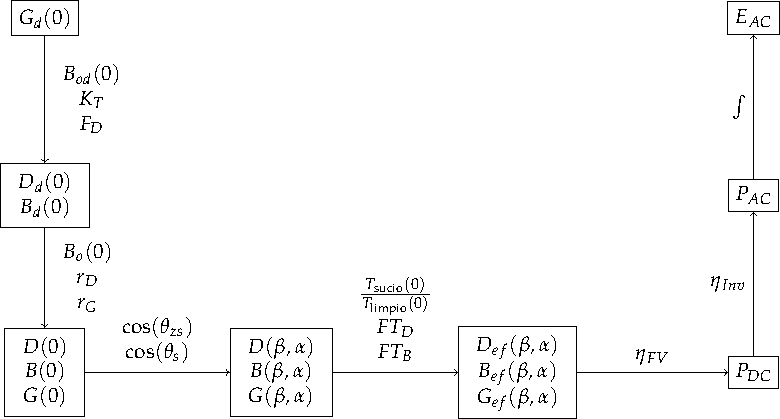
\includegraphics[width=0.8\textwidth]{figuras/ProcedimientoCalculoRadiacionInclinada.pdf}
\caption{\label{fig:orga9d3bdc}El procedimiento de cálculo consiste en obtener la irradiancia efectiva a partir de la irradiación global en un plano horizontal. Primero, se separan las componentes directa y difusa utilizando índices de claridad y fracciones difusas. Luego, se trasladan estos valores al plano inclinado y se ajustan por factores de suciedad y sombras. Con la irradiancia efectiva y la eficiencia del sistema fotovoltaico, se calcula la potencia en corriente continua, que luego se convierte en corriente alterna a través de un inversor. Finalmente, al integrar esta potencia, se obtiene la energía. Figura modificada de la figura 3.3 del libro ESF \cite{Perpinan2023}.}
\end{figure}


El paquete \texttt{solaR2} toma como marco teórico el libro de Oscar Perpiñán, tutor de este trabajo, Energía Solar Fotovoltaica \cite{Perpinan2023} para cada una de las operaciones de cálculo que realizan cada una de las funciones.
En la figura \ref{fig:orga9d3bdc}, se muestra un diagrama que resume los pasos que se siguen a la hora de calcular la producción de sistemas fotovoltaicos.

\FloatBarrier

Estos pasos son:
\begin{enumerate}
\item Calcular la geometría que define la posición relativa del Sol desde la Tierra.
\item Obtener la irradiación global diaria en el plano horizontal
\item A partir de la irradiación global, obtener las componentes de difusa y directa.
\item Se trasladan estos valores de irradiación a valores de irradiancia.
\item Integrando estos valores se pueden obtener las estimaciones irradiación diaria difusa, directa y global
\item El generador fotovoltaico produce una potencia en corriente continua dependiente del rendimiento del mismo.
\item Se transforma en potencia en corriente alterna mediante un inversor que tiene una eficiencia asociada.
\item Integrando esta potencia se puede obtener la energía que produce el generador en un tiempo determinado.
\end{enumerate}


\section{Radiación solar}
\label{sec:orgf26bf27}
\label{radiacion-solar}
\subsection{Geometría Sol y Tierra}
\label{sec:org361336b}
Como es sabido, el movimiento terrestre se compone de una traslación alrededor del Sol y un giro sobre su eje. En este movimiento, la Tierra se desplaza alrededor del Sol siguiendo una elipse de baja excentricidad en la que el Sol ocupa uno de los focos. La duración de este movimiento define un año. La corrección debida a la excentricidad de la elipse\footnote{Correspondiente a la función \texttt{eccentricity}.} se calcula con: \nomenclature[epsilon0]{$\epsilon_0$}{Corrección debida a la excentricidad de la elipse de la trayectoria terrestre alrededor del Sol}
\begin{equation}
\epsilon_0=1+0.033\cdot \cos(\frac{2\pi d_n}{365})
\end{equation}
donde \(d_n\) es el número de día del año (siendo \(d_n=1\) el 1 de Enero). \nomenclature[dn]{$d_n$}{Día del año}

El movimiento que describe la Tierra al girar alrededor del Sol, está contenido en un plano conocido como \emph{plano de la eclíptica}, el cual, entre este y el eje polar (línea imaginaria que uno los dos polos de la Tierra) se forma un ángulo conocido como declinación\footnote{Correspondiente a la función \texttt{declination}}, el cual se puede aproximar de forma sencilla de la siguiente manera\footnote{Por razones de economización del espacio, se va a optar por utilizar las ecuaciones de Cooper \cite{Cooper1969} por su sencillez. Sin embargo, la función \texttt{fSolD} (como se verá en el capítulo \ref{chap:desarrollo-codigo}) puede seleccionar entre 4 tipos de ecuaciones expuestas por diferentes autores (Strous \cite{Strous2011}, Spencer \cite{Spencer1971} y Michalsky \cite{Michalsky1988}).}: \nomenclature[delta]{$\delta$}{Declinación}
\begin{equation}
\delta=23.45^\circ \cdot \sin(\frac{2\pi \cdot (d_n+284)}{365})
\end{equation}

\subsection{Movimiento aparente del sol}
\label{sec:orga6aa03d}
Las variaciones en la declinación hacen que los días fluctuen su duración. Esta duración se puede calcular mediante el ángulo del amanecer\footnote{Correspondiente a la función \texttt{sunrise}.} (\(\omega_s\)), el cúal determina la diferencia angular entre el mediodía solar y el momento en el que amanece. Por lo tango un día durará \(2\cdot |\omega_s|\) (ya que es el ángulo entre el amanecer y el mediodía, y el mediodía y el anochecer). Se puede calcular el ángulo del amanecer de la siguiente manera: \nomenclature[omegas]{$\omega_s$}{Ángulo del amanecer}
\begin{equation}
  \omega_s=\begin{cases}
  -\arccos(-\tan\delta\tan\phi)& \text{si $|\tan\delta\tan\phi|<1$}\\
  -\pi& \text{si $-\tan\delta\tan\phi<-1$}\\
  0& \text{si $-\tan\delta\tan\phi>1$}
  \end{cases}
\end{equation}
donde, \(\phi\) corresponde a la latitud (positiva al norte y negativa al sur). \nomenclature[phi]{$\phi$}{Latitud}

Sin embargo, cada localización tiene una hora oficial, \(TO\), la cual no se corresponde con el ángulo que forma el Sol a lo largo del día, por lo que resulta necesario calcular esta hora solar verdadera (\(\omega\))\footnote{Correspondiente a la función \texttt{sunHour}.}: \nomenclature[TO]{$TO$}{Hora oficial} \nomenclature[omega]{$\omega$}{Hora solar o tiempo solar verdadero}
\begin{equation}
\omega = 15 \cdot (TO-AO-12)+\Delta \lambda + \frac{EoT}{4}
\end{equation}
donde:
\begin{itemize}
\item \(TO\) es la hora oficial.
\item \(AO\) es el adelanto oficial durante el horario de invierno. \nomenclature[AO]{$AO$}{Adelanto oficial durante el horario de invierno}
\item \(\Delta \lambda\) es la diferencia entre la longitud local y la longitud del huso horario. \nomenclature[Deltalambda]{$\Delta \lambda$}{Diferencia entre la longitud local y la longitud del huso horario}
\item \(EoT\) es la ecuación del tiempo\footnote{Correspondiente a la función \texttt{eot}.}, se calcula de la siguiente manera: \nomenclature[EoT]{$EoT$}{Ecuación del tiempo}
\begin{equation}
EoT=229,18\cdot (-0,0334\cdot sin(\frac{2\pi}{365,24}\cdot dn)+0,04184\cdot sin(2\cdot \frac{2\pi}{365,24}\cdot dn+3,5884))
\end{equation}
\end{itemize}

\subsection{Radiación fuera de la atmósfera terrestre}
\label{sec:org6026692}
La radiación extra-atmosférica es la radiación directa del Sol que alcanza la superficie de la atmósfera. El tamaño de la Tierra furente a la distancia que la separa del Sol es muy pequeña, por lo que, es razonable asumir que su valor es constante en toda la superficie exterior de la atmósfera. Se define la constante solar, \(B_0\) como el valor de irradiancia solar incidente en un plano normal al vector Sol-Tierra. Se acepta como representativo el valor promedio de \(B_0=1367W/m^2\).

Para calcular la irradiancia incidente en una superficie tangente a la atmósfera en una latitud determinada (\(B_0(0)\))\footnote{Este cálculo, junto con el de la hora solar, \(\omega\), el coseno del ángulo cenital, \(\theta_{zs}\) y  el ángulo azimutal, \(\psi_s\), se pueden calcular mediante la función \texttt{fSolI}, haciendo uso de sus respectivas funciones.}, se toma la siguiente ecuación: \nomenclature[B00]{$B_0(0)$}{Irradiancia extra-atmosférica o extra-terrestre en el plano horizontal}
\begin{equation}
B_0(0)=B_0 \cdot \epsilon_0 \cdot \cos(\theta_{zs})
\label{eq:irradianciaextra}
\end{equation}
donde, \(\cos(\theta_{zs})\)\footnote{Correspondiente a la función \texttt{zenith}.} es el coseno del ángulo cenital solar\footnote{El ángulo cenital, \(\theta_{zs}\), es el complementario de la áltura solar, \(\gamma_s\).}, y se calcula de la siguiente manera:
\nomenclature[thetazs]{$\theta_{zs}$}{Ángulo cenital solar}
\begin{equation}
cos(\theta_{zs})=cos(\delta)cos(\omega)cos(\phi)+sin(\delta)+sin(\phi)
\end{equation}

Es importate añadir, que con el ángulo cenital, se puede obtener otro ángulo relevante en la geometría solar, se trata del ángulo azimutal, \(\psi_s\)\footnote{Correspondiente a la función \texttt{azimuth}.}, el cual, es el ángulo formado por el meridiano solar y el meridiano del lugar (Sur en el hemisferio Norte y viceversa). \nomenclature[psis]{$\psi_s$}{Ángulo acimutal solar}
\begin{equation}
\cos(\psi_s)=signo(\phi)\cdot \frac{\cos(\delta)\cos(\omega)\cos(\phi)-\cos(\phi)\sin(\delta)}{\sin(\theta_{zs})}
\end{equation}

Para calcular la irradiación diaria extra-atmoférica\footnote{Correspondiente a la función \texttt{bo0d}.}, \(B_{0d}(0)\)\footnote{Este cálculo, junto con la declinación, \(\delta\), la corrección por excentricidad, \(\epsilon_0\), la ecuación el tiempo, \(EoT\), y el ángulo del amanecer, \(\omega_s\), se pueden calcular mediante la función \texttt{fSolD}, haciendo uso de sus respectivas funciones.}, se puede integrar la ecuación \ref{eq:irradianciaextra}:
\nomenclature[B0d0]{$B_{0d}(0)$}{Irradiación diaria extra-atmosférica en el plano horizontal}
\begin{equation}
B_{0d}(0)=-\frac{24}{\pi}B_0\epsilon_0(\omega_s sin\phi sin\delta + cos\phi cos\delta sin \omega_s)
\label{eq:irradiacionextra}
\end{equation}

Es posible demostrar que el promedio mensual de esta irradiación diaria coincide numéricamente con el valor de irradiación diaria correspondiente a los denominados ``días promedios'', días en los que la declinación correpondiente coincide con el promedio mensual (tabla \ref{tab:DiasPromedio})
\begin{center}
{\footnotesize }%
\begin{table}[h]
{\footnotesize \caption{Valor $d_{n}$ correspondiente a los doce días promedio.\label{tab:DiasPromedio}}
}{\footnotesize \par}

\centering{}{\footnotesize }\begin{tabular}{>{\centering}p{6mm}>{\centering}m{4mm}>{\centering}m{4mm}>{\centering}m{4mm}>{\centering}m{4mm}>{\centering}m{4mm}>{\centering}m{4mm}>{\centering}m{4mm}>{\centering}m{4mm}>{\centering}m{4mm}>{\centering}m{4mm}>{\centering}m{4mm}>{\centering}m{3mm}}
\toprule 
{\footnotesize Mes} & {\footnotesize Ene} & {\footnotesize Feb} & {\footnotesize Mar} & {\footnotesize Abr} & {\footnotesize May} & {\footnotesize Jun} & {\footnotesize Jul} & {\footnotesize Ago} & {\footnotesize Sep} & {\footnotesize Oct} & {\footnotesize Nov} & {\footnotesize Dic}\tabularnewline
\midrule
$d_{n}$ & {\footnotesize 17} & {\footnotesize 45} & {\footnotesize 74} & {\footnotesize 105} & {\footnotesize 135} & {\footnotesize 161} & {\footnotesize 199} & {\footnotesize 230} & {\footnotesize 261} & {\footnotesize 292} & {\footnotesize 322} & {\footnotesize 347}\tabularnewline
\bottomrule
\end{tabular}
\end{table}

\par\end{center}{\footnotesize \par}

Todas estas ecuaciones, están recogidas en la función \texttt{calcSol}, la cual computa todos los ángulos solares, diarios e intradiarios, necesarios para la simulación de sistemas fotovoltaicos.

\subsection{Influencia de la atmósfera}
\label{sec:org1c013b6}
La radiación solar, al atravesar la atmósfera, es afectada por reflexión, atenuación y difusión, lo que altera sus características. La reflexión en las nubes reduce la radiación que llega a la Tierra, mientras que la absorción por vapor de agua, ozono y \(CO_2\) cambia el espectro de la radiación. Además, la dispersión por partículas afecta la distribución espacial. Existen tres tipos de difusión según el tamaño de las partículas en interacción:
\begin{itemize}
\item \textbf{Difusión de Rayleigh}: La longitud de onda esmayor que el tamaño de la partícula, ocurre en las capas altas y causa el color azul del cielo.
\item \textbf{Difusión de Mie}: La longitud de onda es similar al tamaño de la partícula, ocurre en las capas bajas.
\item \textbf{Difusión no selectiva}: La longitud de onda es menor que el tamaño de la partícula.
\end{itemize}

Resulta útil definir la masa de aire (\(AM\), \emph{air mass}) como la relación entre el camino recorrido por los rayos directos del Sol a través de la atmósfera hasta la superficie receptora y el que recorerían en caso de incidencia vertical. Se puede aproximar de la siguiente manera: \nomenclature[AM]{$AM$}{Masa de aire}
\begin{equation}
AM = 1/\cos(\theta_{zs})
\end{equation}

Para el cálculo de la irradiancia solar que finalmente incide en una superficie arbitraria localizada en corteza terrestre será útil distinguir tres contribuciones diferentes. Estas contribuciones, comúnmente denominadas componentes, son:
\begin{itemize}
\item \textbf{Radiación Directa}, \(B\): representa la fracción de irradiación procendente en línea recta del Sol. \nomenclature[B]{$B$}{Radiación directa}
\item \textbf{Radiación Difusa}, D\nomenclature[D]{\(D\)}{Radiación difusa}: fracción de radiación que procede de todo el cielo, excepto del Sol. Son todos aquellos rayos que dispersa la atmósfera.
\item \textbf{Radiación del albedo}, R\nomenclature[R]{\(R\)}{Radiación del albedo}: parte de la radiación procedente de la reflexión con el suelo.
\end{itemize}
La suma de las tres componentes constituye la denominada radiación global: \nomenclature[G]{\(G\)}{Radiación global}
\begin{equation}
G = B + D + R
\label{eq:comp_rad}
\end{equation}


\subsection{Cálculo de componentes de radiación solar}
\label{sec:org4761055}
\label{subsec:calculo-componentes-radiacion-solar}
Para caracterizar la radiación solar en un lugar, Liu y Jordan \cite{Liu.Jordan1960} propusieron el índice de claridad, \(K_T\). Este índice es la relación entre la radiación global y la radiación extra-atmosférica, ambas en el plano horizontal. El índice de claridad diario es la relación entre los valores diarios de irradiación: \nomenclature[KT]{\(K_T\)}{Índice de claridad}
\nomenclature[KTd]{\(K_{Td}\)}{Índice de claridad diario}
\begin{equation}
K_{Td}=\frac{G_d(0)}{B_{0d}(0)}
\label{eq:ind-cla-dia}
\end{equation}
mientras que el índice de claridad mensual es la relación entre las medias mensuales de la irradiación diaria:
\nomenclature[KTm]{\(K_{Tm}\)}{Índice de claridad mensual}
\begin{equation}
K_{Tm}=\frac{G_{d,m}(0)}{B_{0d,m}(0)}
\label{eq:ind-cla-men}
\end{equation}

Una vez se tiene el índice de claridad, se puede calcular la fracción de radiación difusa en el plano horizontal. En el caso de medias mensuales \cite{Page1961}:
\begin{equation}
F_{Dm}=1-1,13\cdot K_{Tm}
\end{equation}
Donde:
\begin{itemize}
\item Fracción de radiación difusa: \(F_D=\frac{D(0)}{G(0)}\) \nomenclature[FD]{\(F_D\)}{Fracción de difusa}
\nomenclature[FDd]{\(F_{Dd}\)}{Fracción de difusa diaria} \nomenclature[FDm]{\(F_{Dm}\)}{Fracción de difusa mensual}
\end{itemize}
Al tener la fracción de radiación difusa, se pueden obtener los valores de la radiación directa y difusa en el plano horizontal\footnote{Correpondiente a la familia de funciones \texttt{corrFdKt}.}:
\begin{equation}
D_d(0)=F_D\cdot G_d(0)
\label{dif-rad}
\end{equation}
\begin{equation}
B_d(0)=G_d(0)-D_d(0)
\label{dir-rad}
\end{equation}

Estas expresiones, se recogen en la función \texttt{calcG0}, la cual, calcula las componentes de la irradiancia intradiaria y la irradiación diaria (además de medias mensuales de estas y sumas anuales). Se vale de las funciones \texttt{fCompD}, para la irradiación, y \texttt{fCompI}, para la irradiancia. 

\section{Radiación en superficies inclinadas}
\label{sec:org74b8425}
\label{sec:radiacion-superficies-inclinadas}
Dados los valores de irradiación diaria difusa, directa y global en el plano horizontal se puede realizar la transformación al plano inclinado. Para ello, es necesario estimar el perfil de irradiancia correspondiente a cada valor de irradiación. dado que la variación solar durante una hora es baja, podemos suponer que el valor medio de la irradiancia durante esa hora coincide numéricamente con la irradiación horaria. Por otra parte, el análisis de valores \emph{medios}  en \emph{largas} series temporales ha mostrado que la relación entre la irradiancia y la irradiación extra-atmosférica \cite{Collares-Pereira.Rabl1979} (\ref{eq:rel-dif}):
\begin{equation}
r_D=\frac{D(0)}{D_d(0)}=\frac{B_0(0)}{B_{0d}(0)}
\label{eq:rel-dif}
\end{equation}
Este factor \(r_D\)\nomenclature[rD]{\(r_D\)}{Relación entre la irradiancia y la irradiación difusa en el plano horizontal} es calculable directamente sabiendo que la relación entre irradiancia e irradiación extra-atmosférica es deducible teóricamente a partir de las ecuaciones \ref{eq:irradianciaextra} y \ref{eq:irradiacionextra}:
\begin{equation}
\frac{B_0(0)}{B_{0d}(0)}=\frac{\pi}{T}\cdot \frac{cos(\omega)-cos(\omega_s)}{\omega_s\cdot cos(\omega_s)-sin(\omega_s)}=r_D
\label{eq:rel-dif2}
\end{equation}
el mismo análisis mostró una relación entre la irradiancia e irradiación global asimilable a una función dependiente de la hora solar (\ref{eq:rel-glo}):
\begin{equation}
r_G=\frac{G(0)}{G_d(0)}=r_D\cdot(a+b\cdot cos(w))
\label{eq:rel-glo}
\end{equation}
Donde:
\begin{itemize}
\item \(a=0,409-0,5016\cdot sin(\omega_s+\frac{\pi}{3})\)
\item \(b=0,6609+0,4767\cdot sin(\omega_s+\frac{\pi}{3})\)
\end{itemize}

Es importante resaltar que estos perfiles proceden de medias sobre largos períodos, y de ahí que, como es observable en la figura \ref{fig:orgca6cdce}, las fluctuaciones propias del movimiento de nubes a lo largo del día queden atenuadas y se obtenga una curva sin alteraciones.
\begin{figure}[htbp]
\centering
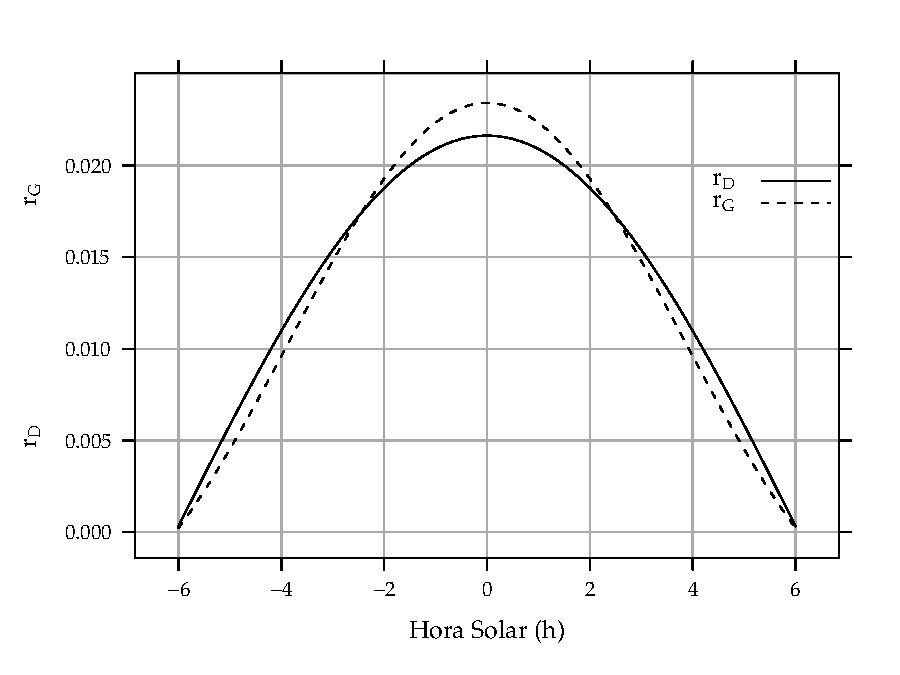
\includegraphics[keepaspectratio,width=0.8\textwidth,height=0.5\textheight]{figuras/RgRd.pdf}
\caption{\label{fig:orgca6cdce}Perfil de irradiancia difusa y global obtenido a partir del generador empírico de \cite{Collares-Pereira.Rabl1979} para valores de irradiancia tomadas cada 10 minutos. Figura 3.4 del libro ESF \cite{Perpinan2023}.}
\end{figure}

\subsection{Transformación al plano del generador}
\label{sec:orga2432a5}
\label{subsec:transformación-plano-generador}
Una vez otenidos los valores de irradiancia en el plano horizontal, se traspone al plano del generador:
\begin{itemize}
\item \textbf{Irradiancia Directa} \(B(\beta ,\alpha)\): Ecuación basada en geometría solar (ángulo zenital) y del generador (ángulo de incidencia).
\begin{equation}
B(\beta ,\alpha)=B(0)\cdot \frac{max(0,cos(\theta_s))}{cos(\theta_{zs})}
\label{eq:irradiancia-directa-plano-generador}
\end{equation}
donde:
\begin{itemize}
\item Ángulo de inclinación: \(\beta\).
\item Ángulo de orientación: \(\alpha\). \nomenclature[alpha]{\(\alpha\)}{Ángulo de orientación de un sistema fotovoltaico}
\end{itemize}
\item \textbf{Irradiancia Difusa} \(D(\beta ,\alpha)\): Utilizando el modelo de cielo anisotrópico \cite{Perpinan2023}, se distinguen dos componentes de la irradiancia difusa, denominados \emph{circunsolar} e \emph{isotrópica}. \nomenclature[DI]{\(D^I\)}{Radiación difusa isotrópica} \nomenclature[DC]{\(D^C\)}{Radiación difusa circunsolar}
\begin{equation}
D(\beta ,\alpha)=D^I(\beta ,\alpha)+D^C(\beta ,\alpha)
\end{equation}
\begin{equation}
D^I(\beta ,\alpha)=D(0)(1-k_1)\cdot \frac{1+cos(\beta)}{2}
\end{equation}
\begin{equation}
D^C(\beta, \alpha)=D(0)\cdot k_1\cdot \frac{max(0,cos(\theta_s))}{cos(\theta_{zs})}
\end{equation}
Donde:
\begin{itemize}
\item \(k_1=\frac{B(n)}{B_0\cdot \epsilon_0}=\frac{B(0)}{B_0(0)}\)
\end{itemize}
\item \textbf{Irradiancia de albedo} \(R(\beta ,\alpha)\): Se considera isotrópica debido a su baja contribución a la radiación global. Se calcula a partir de la irradiancia global en el plano horizontal usando un coeficiente de reflexión, \(\rho\)\nomenclature[rho]{\(\rho\)}{Coeficiente de reflexión del terreno para la irradiancia de albedo}, que depende del terreno. En la ecuación \ref{eq:albedo-plano-generador}, se utiliza el factor \(\frac{1-cos(\beta)}{2}\), complemetario al factor de visión de la difusa isotrópica (figura \ref{fig:org8e0654d})
\begin{equation}
R(\beta ,\alpha)=\rho \cdot G(0)\cdot \frac{1 - cos(\beta)}{2}
\label{eq:albedo-plano-generador}
\end{equation}
\begin{figure}[htbp]
\centering
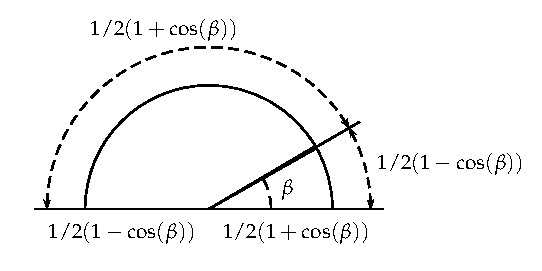
\includegraphics[keepaspectratio,width=0.8\textwidth,height=0.5\textheight]{figuras/AnguloVisionCielo.pdf}
\caption{\label{fig:org8e0654d}Ángulo de visión del cielo. Figura 3.5 del libro ESF \cite{Perpinan2023}.}
\end{figure}
\end{itemize}

\subsection{Ángulo de incidencia y suciedad}
\label{sec:orgaba58e4}
\label{subsec-angulo-incidencia-suciedad}
En un módulo fotovoltaico, la radiación incidente generalmente no es perpendicular a la superficie del módulo, lo que provoca pérdidas por reflexión o pérdidas angulares, cuantificadas por el ángulo de incidencia \(\theta_s\)\nomenclature[thetas]{\(\theta_s\)}{Ángulo de incidencia o ángulo entre el vector solar y el vector director de una superficie}. La suciedad acumulada en la superficie del módulo también reduce la transmitancia del vidrio (representada por \(T_{limpio}(0\))), disminuyendo la irradiancia efectiva, es decir, la radiación que realmente puede ser aprovechada por el módulo.
La irradiancia efectiva para radiación directa se expresa en la ecuación \ref{eq:dir-ef}:
\begin{equation}
B_{ef}(\beta ,\alpha)=B(\beta ,\alpha)\cdot [\frac{T_{sucio}(0)}{T_{limpio}(0)}]\cdot (1-FTB(\theta_s))
\label{eq:dir-ef}
\end{equation}
donde \(FTB(\theta_s)\) es el factor de pérdidas angulares, que se calcula con la ecuación\footnote{Implementada en la función \texttt{fInclin}.} \ref{eq:factor-perdidas-directa}: \nomenclature[FTB]{\(FT_B\)}{Factor de pérdidas angulares para irradiancia directa}\nomenclature[FTD]{\(FT_D\)}{Factor de pérdidas angulares para irradiancia difusa}\nomenclature[FTB]{\(FT_R\)}{Factor de pérdidas angulares para irradiancia de albedo}
\begin{equation}
FTB(\theta_s)=\frac{exp(-\frac{cos(\theta_s)}{a_r})-exp(-\frac{1}{a_r})}{1-exp(-\frac{1}{a_r})}
\label{eq:factor-perdidas-directa}
\end{equation}
Este factor depende del ángulo de incidencia, \(\theta_s\), y del coeficiente de pérdidas angulares, \(a_r\). Cuando la radiación es perpendicular a la superficie (\(\theta_s=0\)), \(FTB\) es cero. En la figura \ref{fig:org3bd6537} se puede observar que las pérdidas angulares son más significativas cuando \(\theta_s\) supera los 60º, y se acentúan con mayor suciedad.
\begin{figure}[htbp]
\centering
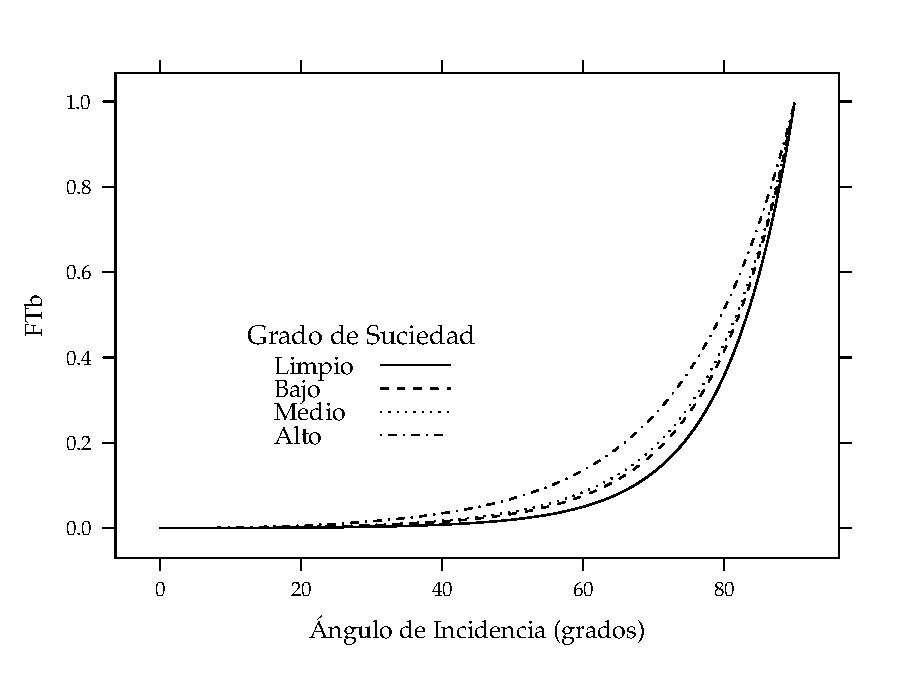
\includegraphics[keepaspectratio,width=0.8\textwidth,height=0.5\textheight]{figuras/Suciedad.pdf}
\caption{\label{fig:org3bd6537}Pérdidas angulares de un módulo fotovoltaico para diferentes grados de suciedad en función del ángulo de incidencia. Figura 3.7 del libro ESF \cite{Perpinan2023}.}
\end{figure}

Para calcular las componente de radiación difusa isotrópica y de albedo se utilizan las ecuaciones\footnote{Implementadas en la función \texttt{fInclin}.} \ref{eq:FTD} y \ref{eq:FTR}:
\begin{equation}
\text{FTD}(\beta) \approx exp[-\frac{1}{a_r}\cdot (c_1\cdot (sin\beta +\frac{\pi -\beta - sin\beta}{1+cos\beta})+c_2\cdot (sin\beta +\frac{\pi -\beta -sin\beta}{1+cos\beta})^2)]
\label{eq:FTD}
\end{equation}
\begin{equation}
\text{FTR}(\beta) \approx exp[-\frac{1}{a_r}\cdot (c_1\cdot (sin\beta +\frac{\beta - sin\beta}{1-cos\beta})+c_2\cdot (sin\beta +\frac{\beta -sin\beta}{1-cos\beta})^2)]
\end{equation}
\label{eq:FTR}
Donde:
\begin{itemize}
\item Ángulo de inclinación del generador (en radianes): \(\beta\) \nomenclature[beta]{\(\beta\)}{Ángulo de inclinación de un sistema fotovoltaico}
\item Coeficiente de pérdidas angulares: \(a_r\)
\item Coeficientes de ajuste: \(c_1\) y \(c_2\) (en la tabla \ref{tab:coef-perd} se recogen algunos valores característicos de un módulo de silicio monocristalino convencional para diferentes grados de suciedad)
\end{itemize}
\begin{table}[htbp]
\caption{Valores del coeficiente de pérdidas angulares y transmitancia relativa en incidencia normal para diferentes tipos de suciedad. \label{tab:coef-perd}}
\centering
\begin{tabular}{lrrr}
\hline
Grado de suciedad & \(\frac{T_{sucio}(0)}{T_{limpio}(0)}\) & a\textsubscript{r} & c\textsubscript{2}\\[0pt]
\hline
Limpio & 1 & 0.17 & -0.069\\[0pt]
\hline
Bajo & 0.98 & 0.20 & -0.054\\[0pt]
\hline
Medio & 0.97 & 0.21 & -0.049\\[0pt]
\hline
Alto & 0.92 & 0.27 & -0.023\\[0pt]
\hline
\end{tabular}
\end{table}

Para estas componenetes el cálculo de irradiancia efectiva es similar al de la irradiancia directa (ecuaciones \ref{eq:dif-ef-iso} y \ref{eq:alb-ef}). Para la componente difusa circunsolar emplearemos el factor de pérdidas angulares de la irradiancia efectiva(ecuacion \ref{eq:dif-ef-cir}):
\begin{equation}
D_{ef}^I(\beta ,\alpha)=D^I(\beta ,\alpha)\cdot[\frac{T_{sucio}(0)}{T_{limpio}(0)}]\cdot (1-FT_D(\beta))
\label{eq:dif-ef-iso}
\end{equation}
\begin{equation}
D_{ef}^C(\beta ,\alpha)=D^C(\beta ,\alpha)\cdot[\frac{T_{sucio}(0)}{T_{limpio}(0)}]\cdot (1-FT_B(\theta_s))
\label{eq:dif-ef-cir}
\end{equation}
\begin{equation}
R_{ef}(\beta ,\alpha)=R(\beta ,\alpha)\cdot[\frac{T_{sucio}(0)}{T_{limpio}(0)}]\cdot (1-FT_R(\beta))
\label{eq:alb-ef}
\end{equation}
Siguiendo el esquema de la figura \ref{fig:orga9d3bdc}, a partir de estas irradiancias efectivas se puede calcular la irradiación global efectiva diaria, mensual y anual\footnote{Correpondiente a la función \texttt{calcGef}.}. Comparando la irradiación global incidente con la irradición efectiva, se puede evaluar el impacto de la suciedad y el desajuste del ángulo en períoods prolongados.

\section{Cálculo de la energía producida por un generador fotovoltaico}
\label{sec:org3a8a24a}
\label{sec:calculo-energia-producida-generador}

\subsection{Funcionamiento de una célula solar}
\label{sec:org21e957a}
\label{subsec:funcionamiento-celula-solar}
Para calcular la energía producida por un generador fotovoltaico, se deben tener en cuenta la influencia de factores tales como la radiación o la temperatura en una célula solar\footnote{Los cálculos de este apartado, quedan recogidos en la función \texttt{fProd}.} y en los valores de tensión y corriente que se alcanzan en dichas condiciones.

Para definir una célula solar, se tomar 4 variables:
\begin{itemize}
\item La corriente de cortocircuito: \(I_{sc}\)
\nomenclature[Isc]{\(I_{sc}\)}{Corriente de cortocircuito de una célula}
\item La tensión de circuito abierto: \(V_{oc}\)
\nomenclature[VOC]{\(V_{oc}\)}{Tensión de circuito abierto de una célula}
\item La corriente en el punto de máxima potencia: \(I_{mpp}\)
\nomenclature[Impp]{$I_{mpp}$}{Corriente de una célula en el punto de máxima potencia}
\item La tensión en el punto de máxima potencia: \(V_{mpp}\)
\nomenclature[Vmpp]{$V_{mpp}$}{Tensión de una célula en el punto de máxima potencia}
\end{itemize}

\subsubsection{Punto de máxima potencia}
\label{sec:org63e088e}
El punto de máxima potencia es aquel situado en la curva de funcionamiento del generador donde, como su propio nombre indica, los valores de tensión y corriente son tales que la potencia que entrega es máxima (figura \ref{fig:org0adb5ac}).
\begin{figure}[htbp]
\centering
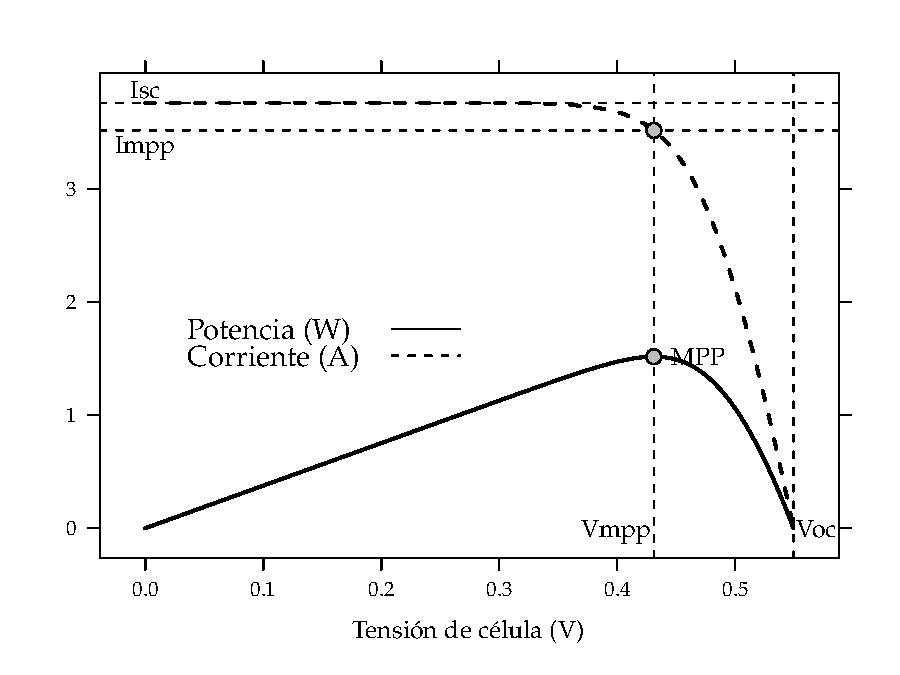
\includegraphics[keepaspectratio,width=0.8\textwidth,height=0.5\textheight]{figuras/CurvaIV_Ta20_G800.pdf}
\caption{\label{fig:org0adb5ac}Curvas corriente-tensión(línea discontinua) y potencia-tensión(línea continua) de una célula solar (\(T_a=20^\circ C\) y \(G=800 W/m^2\)). Figura 4.6 del libro ESF \cite{Perpinan2023}.}
\end{figure}

\subsubsection{Factor de forma y eficiencia}
\label{sec:orgac3dde6}
El área encerrada por el rectángulo definido por el producto \(I_{mpp}\cdot V_{mpp}\) es, como se puede apreciar en la figura \ref{fig:org0adb5ac}, inferiro a la respresentada por el producto \(I_{sc}\cdot V_{oc}\). La relación entre estad dos superficies se cuantifica con el factor de forma:\nomenclature[MPP]{MPP}{Punto de máxima potencia de un dispositivo fotovoltaico}
\begin{equation}
FF=\frac{I_{mpp}\cdot V_{mpp}}{I_{sc}\cdot V_{oc}}
\label{eq:factor-forma}
\end{equation}

Conociendo los valores de \(I_{sc}\) y \(V_{oc}\) es posible calcular la potencia en el punto de máxima potencia, dado que \(P_{mpp}=FF\cdot I_{sc}\cdot V_{oc}\).

Por otra parte, la calidad de una célula se puede cuantificar con la eficiencia de conversión (ecuación \ref{eq:efi-cel}).
\begin{equation}
\eta =\frac{I_{mpp}\cdot V_{mpp}}{P_L}
\label{eq:efi-cel}
\end{equation}
donde \(P_L=A_c\cdot G_{ef}\) representa la potencia luminosa que incide en la célula\nomenclature[Ac]{\(A_c\)}{Área de una célula}. Como es evidente de la ecuación \ref{eq:efi-cel}, este valor de eficiencia se corresponde al caso en el que el acoplamiento entre la carga y la célula permite a esta trabajar en el punto de máxima potencia. En la figura \ref{fig:orgf3c578b} se muestra la evolución temporal del valor de eficiencia de célula de laboratorio para diferentes tecnologías.

\begin{figure}[htbp]
\centering
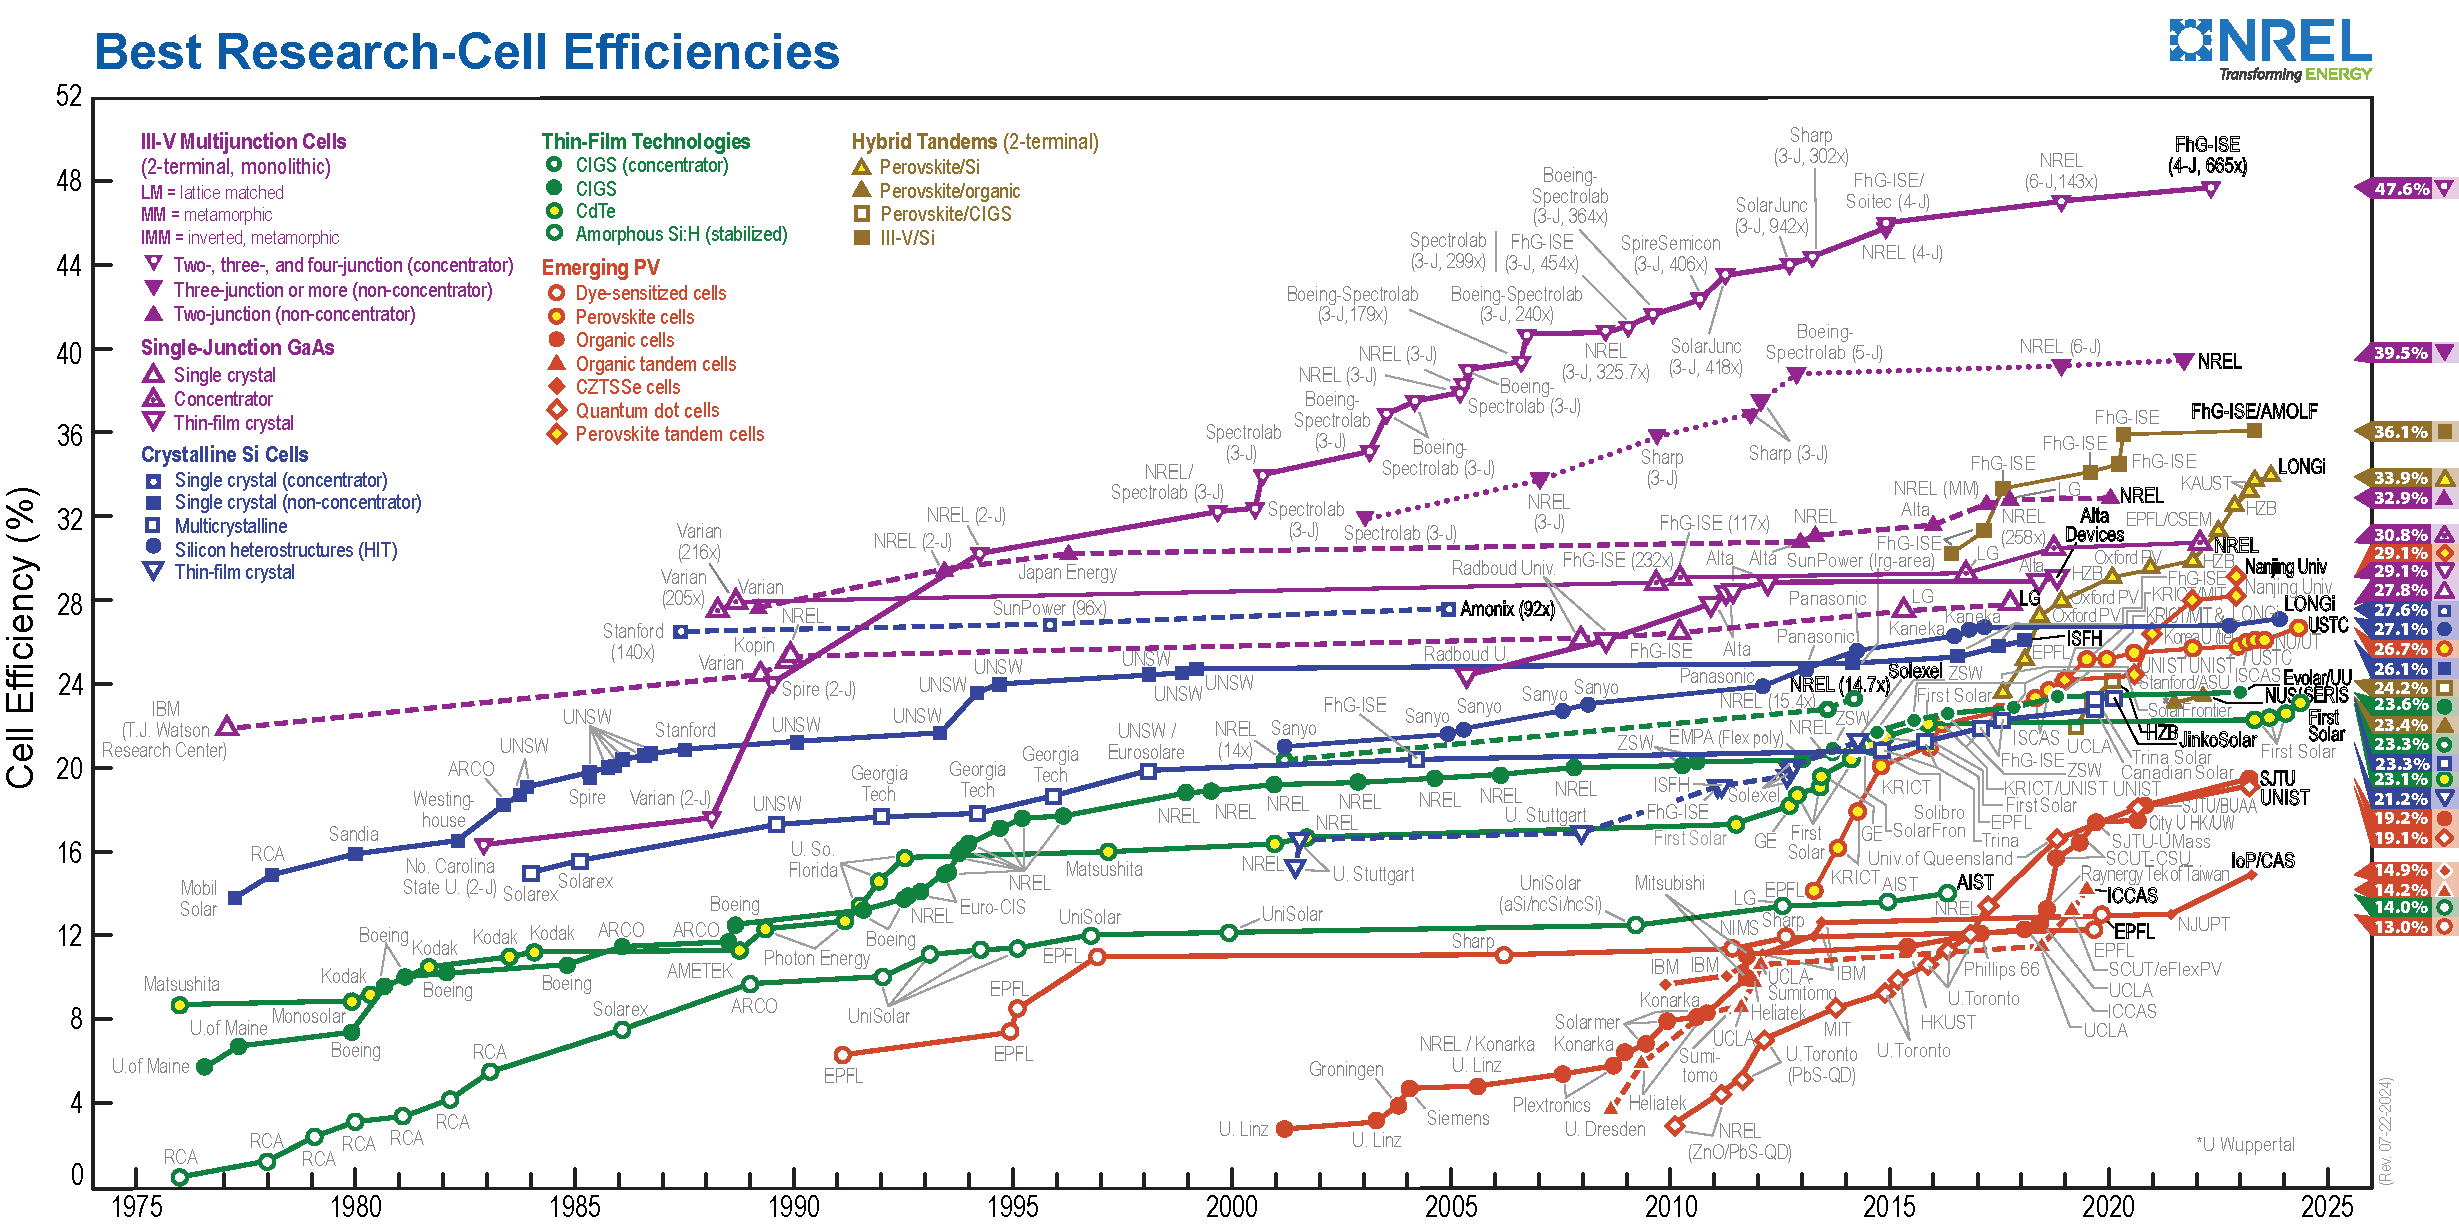
\includegraphics[keepaspectratio,width=0.8\textwidth,height=0.5\textheight]{figuras/cell-efficiencies.pdf}
\caption{\label{fig:orgf3c578b}Evolución de la eficiencia de células según la tecnología (según el National Renewable Energy Laboratory \cite{nrel24} (EEUU)).}
\end{figure}

\subsubsection{Influencia de la temperatura y la radiación}
\label{sec:orgd180348}
La temperatura y la radiación son factores cruciales en el funcionamiento de una célula solar. El aumento de la temperatura ambiente reduce la tensión de circuito abierto según la relación \(dV_{oc}/dT_c\), \nomenclature[Tc]{\(T_c\)}{Temperatura de célula}, que para células de silicio cristalino es de\(-2,3\frac{mV}{^\circ C}\). Además, disminuye la eficiencia de la célula solar con \(\frac{d\eta}{dT_c}=-0,4\%/^\circ C\).

En cuanto a la iluminación, la fotocorriente y la tensíon de circuito abierto son proporcionales a la irradiancia incidente.

Tomando en cuenta estas influencias, se definen una condiciones de funcionamiento, denominadas condiciones estándar de medida(STC)\nomenclature[STC]{STC}{Condiciones estándar de medida de un dispositivo fotovoltaico}, válidas para caracterizar una célula en el entorno de un laboratorio. Estas condiciones vienen determinadas por:
\begin{itemize}
\item Irradiancia: \(G_{stc}=1000W/m^2\) con incidencia normal.
\nomenclature[GSTC]{\(G_{STC}\)}{Irradiancia incidente en condiciones estandar de medida}
\item Temperatura de célula: \(T_c^*=25^\circ C\).\nomenclature[TC*]{\(T_c^*\)}{Temperatura de célula en condiciones estándar de medida}
\item Masa de aire: \(AM=1,5\).\footnote{Relación entre el camino recorrido por los rayos directos del Sol a través de la atmósfera hasta la superficie receptora y el que recorrerían en caso de incidencia vertical (\(AM=1/cos\theta_{zs}\)).}
\end{itemize}
Frecuentemente los fabricantes informan de los valores de las tensiones \(V_{oc}^*\) y \(V_{mpp}^*\) y las corrientes \(I_{sc}^*\) y \(I_{mpp}^*\)\footnote{Es de uso común añadir un asterisco como superíndice para denotar aquellos parámetros medidos en estas condiciones.}. A partir de estos valores es posible referir a estas condiciones:
\begin{itemize}
\item La potencia: \(P_{mpp}^*=I_{mpp}^*\cdot V_{mpp}^*\)
\item El factor de forma: \(FF^*=\frac{P_{mpp}^*}{I_{sc}^*\cdot V_{oc}^*}\)
\item La eficiencia: \(\eta^*=\frac{I_{mpp}^*\cdot V_{mpp}^*}{A_c\cdot G_{stc}}\)
\end{itemize}

\subsection{Funcionamiento de un módulo fotovoltaico}
\label{sec:org8d7cdd6}
\label{subsec:funcionamiento-modulo-fotovoltaico}
\subsubsection{Comportamiento térmico de un módulo}
\label{sec:org81cd3e5}
La mayoría de las ecuaciones que definen el comportamiento de un módulo fotovoltaico\footnote{Los cálculos de este apartado, quedan recogidos en la función \texttt{fProd}.} se establecen en lo que se conocen como condiciones estándar de funcionamiento. En estas condiciones, la temperatura de la célula es de \(25^\circ C\). Sin embargo, la temperatura de operación de la célula es diferente y depende directamente de la radiación que recibe el módulo en cada momento.

El módulo recibe una cantidad de radiación dada, absorbiendo la fracción de esta que no se refleja al exterior. De dicha fracción, parte de ella es transformada en energía eléctrica mientras que el resto se entrega en forma de calor al entorno.

Para simplificar, se puede asumir que el incremento de la temperatura de la célula respecto de la temperatura ambiente depende linealmente de la irradiancia incidente en esta. El coeficiente de proporcionalidad depende de muchos factores, tales como el modo de instalación del módulo, la velocidad del viento, la humedad ambiente y las características constructivas del laminado.

Estos factores quedan recogidos en un valor único representado por la temperatura de operación nominal de célula (NOCT o TONC)\nomenclature[TONC]{\(TONC\)}{Temperatura de operación nominal de célula}, definida como aquella que alcanza una \emph{célula} cuando su \emph{módulo} trabaja en las siguientes condiciones:
\begin{itemize}
\item Irradiancia: \(G=800W/m^2\).
\item Masa de aire: \(AM= 1,5\).
\item Irradiancia normal.
\item Temperatura \emph{ambiente}: \(T_a=20^\circ C\).
\item Velocidad de viento: \(v_v=1m/s\).
\end{itemize}

La ecuación \ref{eq:temp-cel} expresa una aproximación aceptable del comportamiento térmico de una célula integrada en un módulo en base a las consideraciones previas:
\begin{equation}
T_c=T_a+G_{ef}\cdot \frac{NOCT-20}{800}
\label{eq:temp-cel}
\end{equation}
Para la simulación del funcionmaiento de un módulo fotovoltaico en condiciones de operación real, es necesario contar con secuencias de valores de temperatura ambiente. Si no se dispone de información detallada, se puede asumir un valor constante de \(T_a=25^\circ C\) para simulaciones anuales. Sin embargo, si se conocen los valores máximos y mínimos diarios de la temperatura ambiente, se puede generar una secuencia intradiaria usando una combinación de funciones coseno:
\begin{enumerate}
\item \textbf{Calcular los valores de} \(T_m\) \textbf{y} \(T_r\): Se definen los valores de la temperatura media diaria, \(T_m\) simplemente como la media entre la \(T_{max}\) y la \(T_{min}\):
\nomenclature[Tmax]{$T_{max}$}{Temperatura máxima en un día}
\nomenclature[Tmin]{$T_{min}$}{Temperatura mínima en un día}
\begin{equation}
T_m=\frac{T_{max}+T_{min}}{2}
\end{equation}
y la mitad de la amplitud de temperaturas, \(T_r\):
\begin{equation}
T_r=\frac{T_{max}-T_{min}}{2}
\end{equation}
\item \textbf{Calcular la matriz de} \(T_a\): Una vez obtenidos los valores de \(T_m\) y \(T_r\), el siguiente paso es calcular la matriz de valores de temperatura ambiental \(T_a\) para cada hora. Para ello, se deben calcular 3 valores auxiliares:
\nomenclature[Ta]{Ta}{Temperatura ambiente}
\begin{equation}
a_1=\frac{12\pi \cdot (\omega_s-\omega)}{21\pi+12\cdot \omega_s}
\end{equation}
\begin{equation}
a_2=\frac{\pi \cdot (3\pi -12\omega)}{3\pi - 12\omega}
\end{equation}
\begin{equation}
a_3=\frac{\pi (24\pi + 12 \cdot (\omega_s - \omega))}{21 \cdot \pi + 12 \cdot \omega_s}
\end{equation}
Con estos tres valores se pueden calcular la terna de temperaturas \(T_1\), \(T_2\), \(T_3\):
\begin{equation}
T_1 = T_m-T_r\cdot\cos(a_1)
\end{equation}
\begin{equation}
T_2 = T_m+T_r\cdot\cos(a_2)
\end{equation}
\begin{equation}
T_3=T_m-T_r\cdot\cos(a_3)
\end{equation}
\item \textbf{Selección del valor clave}: Se selecciona el valor adecuado de \(T_a\) en base al siguiente criterio:
\begin{equation}
T_a = \begin{cases}
T_1& \text{si $\omega \leq \omega_s$}\\
T_2& \text{si $\omega_s < \omega \leq \frac{\pi}{4}$}\\
T_3& \text{si $\omega > \frac{\pi}{4}$}
\end{cases}
\end{equation}
\end{enumerate}
\subsubsection{Cálculo de \(V_{oc}\) y \(I_{sc}\)}
\label{sec:orgf2ef35d}
Conociendo ya los valores horarios de temperatura de la célula, se puede calcular \(V_{oc}\) utilizando la ecuación \ref{eq:ten-ca}. Y, por último, mediante la ecuación \ref{eq:int-cc} se puede calcular \(I_{sc}\).
\begin{equation}
V_{oc}(T_c)=V_{oc}^*+(T_c-T_c^*)\cdot \frac{dV_{oc}}{dT_c}\cdot N_{cs}
\label{eq:ten-ca}
\end{equation}
\begin{equation}
I_{sc}=G_{ef}\cdot \frac{I_{sc}^*}{G^*}
\label{eq:int-cc}
\end{equation}

\subsubsection{Factor de forma variable}
\label{sec:org42c03c5}
Una vez obtenidos los valores de \(V_{oc}\) y \(I_{sc}\), el siguiente paso ha de ser calcular los valores de tensión y corriente en el punto de máxima potencia, pues es donde el generador estará entregando su máxima potencia, como su propio nombre indica, y por tanto es un punto de interés para el cálculo.

Existen dos metodologías de cálculo de dicho punto, uno de ellos significantemente más sencillo que el otro. este consiste en suponer que el Factor de Forma, definido en la expresión \ref{eq:factor-forma} es constante.

Si suponemos que FF es constante, se podrían extraer los valores de tensión y corriente en el punto de máxima potencia ya que si
\begin{equation}
FF=FF^*
\end{equation}
entonces
\begin{equation}
\frac{I_{mpp}\cdot V_{vmpp}}{I_{sc}\cdot V_{oc}}=\frac{I_{mpp}^*\cdot V_{vmpp}^*}{I_{sc}^*\cdot V_{oc}^*}
\end{equation}
pudiendo así obtener los valores de \(I_{mpp}\) y \(V_{vmmp}\).

Sin embargo, este suposición da resultados alejados a una estimación acertada. Por ello, se tendrá en cuenta la variación del factor de forma:
\begin{itemize}
\item \textbf{Cálculo de la tensión termica, \(V_t\), a temperatura de la célula}: Se calculará el valor de \(V_t\) a 25ºC con la expresión:
\begin{equation}
V_{tn}=\frac{V_t\cdot (273+25)}{300}
\end{equation}
\item \textbf{Cálculo de \(R_s^*\)}: El segundo paso consiste en calcular el valor de resistencia en serie con los valores STC:
\begin{equation}
R_s^*=\frac{\frac{V_{oc}^*}{N_{cs}}-\frac{V_{mpp}^*}{N_{cs}}+m\cdot V_{tn}\cdot ln(1-\frac{I_{mpp}^*}{I_{sc}^*})}{\frac{I_{mpp}^*}{N_{cp}}}
\end{equation}
\item \textbf{Cálculo de \(r_s\)}: Utilizando el valors de \(R_s^*\) calculado en el paso anterior junto con los valores de \(V_{oc}\) y \(I_{sc}\) podemos calcular \(r_s\) que se utilizará más adelante en el proceso.
\begin{equation}
r_s=R_s^*\cdot (\frac{N_{cs}}{N_{cp}}\cdot \frac{I_{sc}}{V_{oc}})
\end{equation}
\item \textbf{Cálculo de \(k_{oc}\)}: A continuación, utilizando los valores de temperatura ambiente obtenidos con anterioridad junto con la tensión de circuito abierto, se calcula \(k_{oc}\) mediante la expresión:
\begin{equation}
k_{oc}=\frac{V_{oc}/N_{cs}}{m\cdot V_t \cdot \frac{T_c+273}{300}}
\end{equation}
\end{itemize}

Con estos cálculos previos, este método propone localizar el punto de máxima potencia de forma aprodimada mediante la ecuaciones:
\begin{equation}
i_{mpp}=1-\frac{D_M}{k_{oc}}
\end{equation}
\begin{equation}
v_{mpp}=1-\frac{ln(k_{oc}/D_M)}{k_{oc}}-r_s\cdot i_{mpp}
\end{equation}
donde:
\begin{equation}
D_M=D_{M0}+2\cdot r_s\cdot D_{M0}^2
\end{equation}
\begin{equation}
D_{M0}=\frac{k_{oc}-1}{k_{oc}-lnk_{oc}}
\end{equation}

Por último, multiplicando los valores de \(i_{mpp}\) y \(v_{mpp}\) por \(I_{sc}\) y \(V_{oc}\) respectivamente, se obtienen los valores de \(I_{mpp}\) y \(V_{mpp}\) que serán los que se utilicen para calcular la potencia entregada por el generador en el punto de máxima potencia.

Teniendo estos valores se puede obtener:
\begin{equation}
P_{mpp}=I_{mpp}\cdot V_{mpp}
\end{equation}

\subsection{Cálculo de potencias y energías de un sistema fotovoltaico conectado a la red}
\label{sec:orgfce2fcc}
\label{subsec:calculo-potencias-energias}
La potencia obtenida en el paso anterior es la de un solo módulo. Para conocer la potencia que va a ser capaz de entregar un SFCR, se debe tener en cuenta su configuración de módulos en serie y en paralelo\footnote{Los cálculos de este apartado, quedan recogidos en las funciones \texttt{fProd} y \texttt{prodCGPV}.}.
\begin{equation}
P_g^*=N_s\cdot N_p\cdot P_m^*
\end{equation}
Con este paso se obtiene la potencia horaria entregada por el generador fotovoltaico. El siguiente paso será pasar esa potencia a través del inversor y calcular la potencia a la salida de este.

Primero, se esteblecen las expresiones de las potencias normalizadas. Siendo \(P_{inv}\) la potencia nominal del inversor:
\nomenclature[Pinv]{\(P_{inv}\)}{Potencia nominal de un inversor}
\begin{equation}
p_i=\frac{P_{DC}}{P_{inv}}
\end{equation}
\begin{equation}
p_o=\frac{P_{AC}}{P_{inv}}
\end{equation}

Por otro lado, el rendimiento de un inversor fotovoltaico se puede modelizar de la siguiente manera:
\begin{equation}
\eta_{inv}=\frac{p_o}{p_o+k_0+k_1p_o+k_2p_o^2}
\end{equation}

De las dos ecuaciones anteriores se puede deducir:
\begin{equation}
p_i=p_o+k_0+k_1p_o+k_2p_o^2
\end{equation}

Desarrollando esta ecuación, se puede obtener una ecuación de segundo grado con \(p_o\) como incógnita:
\begin{equation}
k_2p_o^2+(k_1+1)p_o+(k_0-p_i)=0
\end{equation}

Por último, volviendo a las primeras expresiones se puede obtener la potencia en corriente alterna:
\begin{equation}
P_{AC}=p_o\cdot P_{inv}
\end{equation}

Con esta potencia, integrando en función del tiempo se puede obtener la energía que genera el sistema
\begin{equation}
E_{AC}=\int_{T} P_{AC} \,dt
\end{equation}
y la productividad:
\begin{equation}
Y_f=\frac{E_{ac}}{P_g^*}
\end{equation}

\subsection{Cálculo de potencias y energías de un sistema fovoltaico de bombeo}
\label{sec:orgf16ce8b}
\subsubsection{Potencia hidráulica}
\label{sec:org7afc0d5}
La potencia hidráulica, \(P_H\) \nomenclature[PH]{$P_H$}{Potencia hidráulica}, necesaria para bombear agua es función de,
\begin{itemize}
\item La altura vertical aparente, \(H_v\) \nomenclature[Hv]{$H_v$}{Altura vertical aparente}
\item El caudal de agua, \(Q\) \nomenclature[Q]{$Q$}{Caudal de agua} \nomenclature[g]{$g$}{Aceleración de la gravedad} \nomenclature[rho]{$\rho$}{Densidad del agua}
\end{itemize}
\begin{equation}
P_H=g\cdot \rho \cdot Q \cdot H_V
\end{equation}

Expresando \(P_H\) en watios, \(H_v\) en metros y \(Q\) en \(m^3/h\) la ecuación resulta en:
\begin{equation}
P_H=2.725\cdot Q \cdot H_v
\end{equation}

Asumiendo que el agua bombeado sale por el coducto a baja velocidad, la potencia de salida de la bomba necesita satisfacer \(P_H\) \nomenclature[PH]{$P_H$}{Potencia hidraúlica necesaria en un sistema de bombeo de agua} más las pérdidas de fricción en la tubería, \(P_f\) \nomenclature[Pf]{$P_f$}{Pérdidas de frición en la tubería de un sistema de bombeo}. Este valor se asimila a una altura equivalente \(H_f\) \nomenclature[Hf]{$H_f$}{Altura asociada a las pérdidas de frición en una tubería} asociado a un caudal determinado: \nomenclature[HT]{$H_T$}{Altura total incluyendo las pérdidas de fricción de la tubería}
\begin{equation}
H_T=H_v+H_f
\end{equation}
La potencia eléctrica a la entrada de la motobomba, \(P_{el}\), es:
\nomenclature[Pel]{$P_{el}$}{Potencia eléctrica necesaria en la entrada de una motobomba}
\begin{equation}
P_{el}=\frac{P_H+P_f}{\eta_{mp}} 
\end{equation}
donde \(\eta_{mp}\) es la eficiencia de la motobomba.
\nomenclature[etamp]{$\eta_{mp}$}{Eficiencia de una motobomba}
La potencia eléctrica requerida por la motobomba es entregada por un generador FV y acondicionador de potencia:
\begin{equation}
P_{el}=P_g^* \cdot \frac{G}{G_{stc}} \frac{\eta_g}{\eta_g^*} \cdot \eta_{inv}
\end{equation}
siendo \(G\) la irradiancia en el plano del generador, \(eta_{inv}\) la eficiencia del equipo de acondicionamiento de potencia y \(\frac{\eta_g}{\eta_g^*}\) modela el comportamiento del generador con la temperatura.

\subsubsection{Caudal diario}
\label{sec:orga5dd79f}
El caudal diario bombeado por este conjunto es:
\begin{equation}
Q_d = \int_{d} \frac{G}{G^*} \cdot P_g^* \cdot \eta_g \cdot \frac{\eta_{ig}}{\eta_{ig}^*} \cdot \eta_{inv} \cdot \eta_{mp} \, dt
\end{equation}

\subsubsection{Altura}
\label{sec:orge336c0c}
Se puede definir una altura total equivalente, \(H_{TE}\), con las siguientes suposiciones:
\nomenclature[HTE]{$H_{TE}$}{Altura total equivalente de un sistema de bombeo}
\begin{itemize}
\item Las pérdidas de fricción en tubería son despreciables (\(H_f < 0.05 \cdot H_T\)).
\item El nivel del agua dentro del pozo se mantiene constante.
\end{itemize}
\begin{equation}
Q_d = \frac{P^*_g}{2.725 \cdot G^* \cdot H_{TE}} \int \left( \frac{G}{\eta_{ig}^{*} \eta_{m}^{*} \eta_{inv} \eta_{mp}} \right) dt
\end{equation}
Ahora el cálculo en la integral sólo depende de la radiación, temperatura, y equipos.

Para calcular esta altura total equivalente, se debe suponer que:
\begin{itemize}
\item El pozo está caracterizado con tres parámetros:
\begin{itemize}
\item Nivel estático, \(H_{st}\).
\nomenclature[Hst]{$H_{st}$}{Nivel estático de un pozo}
\item Nivel dinámico, \(H_{dt}\).
\nomenclature[Hdt]{$H_{dt}$}{Nivel dinámico de un pozo}
\item Caudal de ensayo, \(Q_t\). \nomenclature[Qt]{$Q_t$}{Caudal de ensayo de un pozo}
\end{itemize}
\item Que se ha realizado el ensayo de bombeo para caracterizar los pozos con bomba portátil empleando el caudal máximo del pozo, \(Q_{max}\) (\(Q_t=Q_{max}\)).
\nomenclature[Qman]{$Q_{max}$}{Caudal máximo del pozo}
\end{itemize}

Con estas suposiciones se puede llegar a la expresión:
\begin{equation}
H_{TE} = H_{ot} + H_{st} + \left( \frac{H_{dt} - H_{st}}{Q_T} \right) Q_{AP} + H_f(Q_{AP})
\end{equation}
donde:
\begin{itemize}
\item \(H_{OT}\), es la altura desde la salida de agua hasta el suelo.
\nomenclature[HOT]{$H_{OT}$}{Diferencia de cotas entre la salida de agua y la entrada en el depósito}
\item Nivel estático, \(H_{st}\).
\item Nivel dinámico, \(H_{dt}\).
\item Caudal aparente, \(Q_{AP} = \alpha \cdot Q_d\)
(\(\alpha=1/24=0.0416h^{-1}\)).
\item \(H_f(Q_{AP})\), pérdidas en la tubería al caudal aparente.
\end{itemize}

\subsubsection{Potencia del generador}
\label{sec:orgfa86f91}
Como primera aproximación, se consideran constantes a lo largo del tiempo las eficiencias de los componentes del sistema con la elección de ciertos valores adecuados (\(\frac{\eta_g}{\eta_g^*}=0.85, \eta_{mp}=0.35, \eta_{inv}=0.9\)). Así, es posible calcular de forma aproximada la potencia nominal del generador necesaria para bombear un caudal diario \(Q_d\) a una altura total equivalente \(H_{TE}\) a partir de la ecuación:
\begin{equation}
P^*_g = \frac{10 \cdot HTE \cdot Q_d}{\frac{G_d}{G_{stc}}}
\end{equation}

\subsubsection{Simulación de sistemas fotovoltaicos de bombeo}
\label{sec:orgd70630b}
Debido a la complicación del cálculo del dimensionamiento de los sistemas fotovoltaicos de bombeo, se puede recurrir a métodos de simulación asistidos por ordenador\footnote{Correspondientes a la función \texttt{fPump}.}. El algoritmo a seguir es:
\begin{enumerate}
\item Curva característica de la bomba que relaciona la altura, \(H\), y el caudal, \(Q\), a la frecuencia nominal de la bomba:
\begin{equation}
H = a \cdot f^2 + b \cdot f \cdot Q + c \cdot Q^2
\end{equation}
\begin{itemize}
\item Donde \(a\), \(b\), y \(c\) son coeficientes característicos de la bomba y \(f\) es la frecuencia.
\end{itemize}
\item Relaciones de semejanza para bombas centrífugas:
\begin{equation}
\frac{f_1}{f_2} = \frac{Q_1}{Q_2} = \left(\frac{H_1}{H_2}\right)^{1/2} = \left(\frac{P_1}{P_2}\right)^{1/3}
\end{equation}
\item Cálculo de caudal y altura a frecuencia nominal (50 Hz):
\begin{equation}
Q_{50} = \frac{50 \cdot Q}{f}
\end{equation}
\begin{equation}
H_{50} = H \cdot \left(\frac{50}{f}\right)^2
\end{equation}
\item Ecuación de potencia hidráulica:
\begin{equation}
P_{h,50} = 2.725 \cdot Q_{50} \cdot H_{50}
\end{equation}
\item Potencia mecánica en el eje de la bomba a 50 Hz:
\begin{equation}
P_{b,50} = \frac{P_{h,50}}{\eta_b}
\end{equation}
\item Potencia mecánica a frecuencia \(f\):
\begin{equation}
P_b = P_{b,50} \cdot \left(\frac{f}{50}\right)^3
\end{equation}
\item Potencia eléctrica demandada por el motor:
\begin{equation}
P_{bc} = P_b \cdot \frac{50}{f}
\end{equation}
\begin{equation}
P_{e,50} = \frac{P_{bc}}{\eta_m}
\end{equation}
\begin{equation}
P_e = P_{e,50} \cdot \frac{f}{50}
\end{equation}
\item Perfil de irradiancia diaria (según IEC 61725):
\begin{equation}
G = G_{max} \cdot \cos\left(\frac{t}{t_0} \cdot \frac{\pi}{2}\right) \cdot \left[1 + s \cdot \left(1 - \cos\left(\frac{t}{t_0} \cdot \frac{\pi}{2}\right)\right)\right]
\end{equation}
donde G es la irradiancia (\(W/m^2\)) en la hora \(t\), \(G_{max}\) es el valor máximo de irradiancia (\(W/m^2\)) dureante el día en cuestión, y \(s\) es el facotor de forma definido por:
\begin{equation}
s = \frac{d \cdot \frac{\pi}{2} - 1}{1 - \frac{\pi}{4}}
\end{equation}
siendo \(d\) el factor de conjunto de datos calculado con:
\begin{equation}
d = \frac{G_d}{G_{max} \cdot h}
\end{equation}
\end{enumerate}

\section{Sombras y ocupación de terreno}
\label{sec:org592359c}
Al diseñar una central fotovoltaica se debe decidir la ubicación de las diferentes partes del generador resolviendo un compromiso entre la mejor ocupación del terreno disponible y la minimización del impacto de sombras mutuas arrojadas entre los módulos\footnote{Correpondiente a las funciones \texttt{calcShd} (cálculo de sombras) y \texttt{optimShd} (optimización de distancias).}.

Este factor de sombras implica un nivel de ocupación de terreno que depende del modo de seguimiento del generador. La ocupación del terreno se puede medir con dos métricas:
\begin{itemize}
\item \textbf{Relación de ocupación del terreno} (\emph{Ground Coverage Ratio}, \(GCR\)): es la relación entre el área del generador, \(A_G\), y el área del terreno ocupado, \(A_T\) (por tanto, siempre será GCR < 1). \nomenclature[AG]{$A_G$}{Área de un generador fotovoltáico} \nomenclature[GCR]{$GCR$}{Ground coverage ratio}
\begin{equation}
GCR = \frac{A_G}{A_T}
\end{equation}
\item \textbf{Ratio de ocupación del terreno} (\(ROT\), o \emph{Ground Requirement Ratio}, \(GRR\)): es el inverso del GCR, la relación entre el área de terreno ocupado, \(A_T\), y el área del generador, \(A_G\). \nomenclature[ROT]{$ROT$}{Ratio de ocupación del terreno}
\begin{equation}
ROT = \frac{A_T}{A_G}
\end{equation}
\end{itemize}

\subsection{Sistemas estáticos}
\label{sec:org22c7499}
Las filas que componen el generador arrojan sombras unas sobre otras en determinados momentos del días y año. Como recomendación general, es de uso común respetar un mínimo de 4 horas de sol en torno al mediodía del solsticio de invierno libres de sombra. La longitud de la sombra de un obstáculo se mide con:
\begin{equation}
d = \frac{h}{tan\gamma_s}
\end{equation}
siendo \(h\) la altura de la fila adyacente, \(h=L\cdot sin(\beta)\) y \(L\) la longitud del generador, según se indica en la figura \ref{fig:sombras-estaticos}.
\begin{figure}[htbp]
\centering
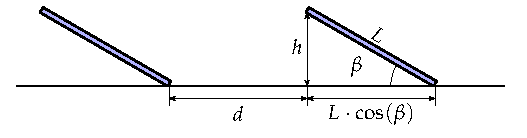
\includegraphics[width=.9\linewidth]{figuras/SombrasEstaticas.pdf}
\caption{Dimensiones y distancias entre filas de un sistema estático. Figura 6.10 del libro ESF \cite{Perpinan2023}. \label{fig:sombras-estaticos}}
\end{figure}

En el mediodía del solsticio de invierno la altura solar es \(\gamma_s = 90^\circ - 23.45^\circ - |\phi| \simeq 67^\circ - |\phi|\). Por tanto, la distancia mínima que permite 4 horas libres de sombra alrededor del mediodía es:
\nomenclature[dmin]{$d_{min}$}{Distancia mínima entre hileras de un generador para evitar el sombreado}
\begin{equation}
d_{min}=\frac{h}{tan(61^\circ - |\phi|)}
\end{equation}

\subsection{Sistemas de seguimiento a doble eje}
\label{sec:org87d2c5c}
El diseño de un sistema de seguimiento solar a doble eje busca optimizar la ubicación de los seguidores para minimizar las pérdidas de radiciación por sombras, utilizando eficientemente el terreno. Para esto, se simula el sistema en diferentes configuraciones y se elige la más eficiente en términos de productividad y ROT, que se calcucula con la fórmula:
\begin{equation}
ROT = \frac{L_{ns}\cdot L_{eo}}{L\cdot W}
\end{equation}
donde (figuras \ref{fig:sombras-doble} y \ref{fig:dimensiones-sombras-doble}):
\begin{itemize}
\item \(L_{ns}\) es la separación entre seguidores en la dirección Norte-Sur.
\nomenclature[Lns]{$L_{ns}$}{Separación entre seguidores en sentido Norte-Sur}
\item \(L_{eo}\) es la separación en la dirección Este-Oeste.
\nomenclature[Leo]{$L_{eo}$}{Separación entre seguidores en sentido Este-Oeste}
\item \(L\) es la longitud del seguidor.
\item \(W\) es la anchura del seguidor.
\end{itemize}

\begin{figure}[htbp]
\centering
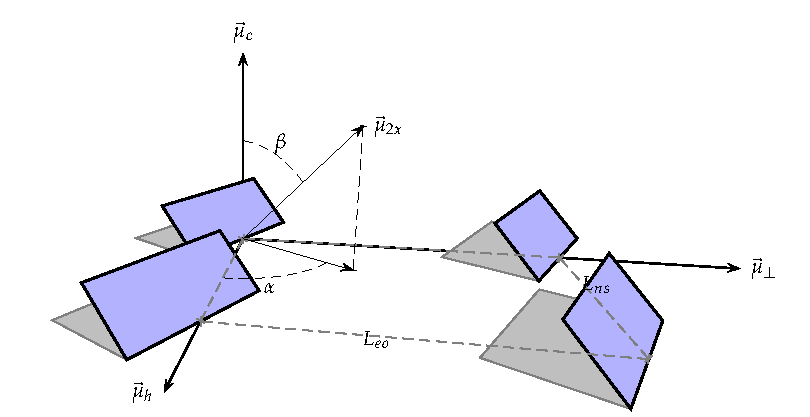
\includegraphics[height=0.2\textheight]{figuras/Sombras2X.pdf}
\caption{Sombras mutuas en un conjunto de cuatro seguidores. Figura 6.11 del libro ESF \cite{Perpinan2023}. \label{fig:sombras-doble}}
\end{figure}
\begin{figure}[htbp]
\centering
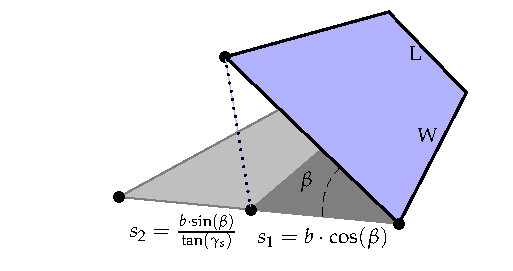
\includegraphics[height=0.2\textheight]{figuras/DimensionesSeguidorSombra.pdf}
\caption{Dimensiones de un seguidor a doble eje y longitud de su sombra arrojada. Figura 6.12 del libro ESF \cite{Perpinan2023}. \label{fig:dimensiones-sombras-doble}}
\end{figure}
\begin{figure}[htbp]
\centering
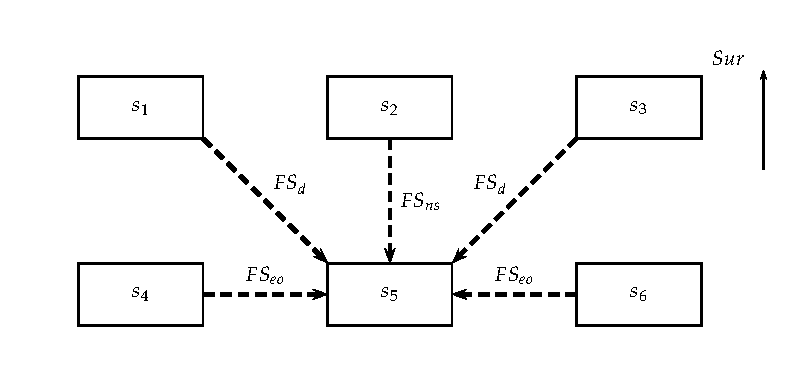
\includegraphics[height=0.2\textheight]{figuras/SixTrackerShadow.pdf}
\caption{Posibles sombras en un conjunto de seis seguidores. Figura 6.13 del libro ESF \cite{Perpinan2023}. \label{fig:conjunto-seis-seguidores}}
\end{figure}


El sistema se modela como un grupo de seis seguidores en una matriz de dos filas en dirección Norte-Sur (figura \ref{fig:conjunto-seis-seguidores}), representando tres situaciones de sombra: lateral (Este-Oeste), frontal (Norte-Sur) y diagonal, caracterizados por los factores de sombra \(FS_{xx}\), definidos como la relación entre el área sombreada y el área total del generador. Las ecuaciones para estos factores son, en las que se emplean los valores normalizados de las distancias, \(l_{eo}=\frac{L_{eo}}{W}\) y \(l_{ns}=\frac{L_{ns}}{W}\):
\begin{equation}
\begin{array}{c}
|l_{eo}\cdot\cos(\psi_{s})|<1\\
|l_{eo}\cdot\sin(\psi_{s})|<s\end
{array}
\Rightarrow
FS_{eo}=\frac{(1-|l_{eo}\cos(\psi_{s})|)\cdot(s-|l_{eo}\sin(\psi_{s})|)}{s}
\end{equation}
\begin{equation}
\begin{array}{c}
|l_{ns}\cdot\cos(\psi_{s})|<s\\
|l_{ns}\cdot\sin(\psi_{s})|<1
\end{array}
\Rightarrow 
FS_{ns}=\frac{(s-|l_{ns}\cos(\psi_{s})|)\cdot(1-|l_{ns}\sin(\psi_{s})|)}{s}
\end{equation}
\begin{align*}
\begin{array}{c}
s>|l_{ns}\cdot\cos(\psi_{s})|+|l_{eo}\sin(\psi_{s})|\\
1>|l_{eo}\cdot\cos(\psi_{s})|-|l_{ns}\cdot\sin(\psi_{s})|
\end{array} 
& \Rightarrow
\end{align*}
\begin{equation}
FS_{d}=\frac{\left[s-\left(|l_{eo}\cdot\sin(\psi_{s})|+|l_{ns}\cos(\psi_{s})|\right)\right]\cdot\left[1-\left(|l_{eo}\cdot\cos(\psi_{s})|-|l_{ns}\sin(\psi_{s})|\right)\right]}{s}
\end{equation}
siendo \(\psi_{s}\) el acimut solar y \(\gamma_{s}\) la altura solar y donde la longitud de sombra (normalizada con la anchura del seguidor) se calcula con:
\begin{align}
s & =s_{1}+s_{2}\\
s_{1} & =b\cdot\cos(\beta)\\
s_{2} & =\frac{b\cdot\sin(\beta)}{\vert\tan(\gamma_{s})\vert}
\end{align}
El factor \(\frac{\sin(\gamma_{s})}{\sin(\gamma_{s}+\beta)}\) representa 
la proyección de sombra existente en el suelo sobre el plano del generador, y por tanto, el porcentaje de área sombreada que debe ser eliminado de la radiación directa. Desarrollando este factor se obtiene una formulación alternativa que puede facilitar el cálculo de los tres factores:
\begin{align}
FS_{eo} & =\frac{(1-l_{eo}\cos(\psi_{s}))\cdot(s-l_{eo}\sin(\psi_{s}))}{s}\\
FS_{ns} & =\frac{(s-l_{ns}\cos(\psi_{s}))\cdot(1-l_{ns}\sin(\psi_{s}))}{s}\\
FS_{d} & =\frac{\left[s-\left(l_{eo}\cdot\sin(\psi_{s})+l_{ns}\cos(\psi_{s})\right)\right]\cdot\left[1-\left(l_{eo}\cdot\cos(\psi_{s})-l_{ns}\sin(\psi_{s})\right)\right]}{s}
\end{align}

Realizando la simulación de este sistema incluyendo el cálculo de sombras, y repitiendo la simulación para varias combinaciones (Lns, Leo) pueden elaborarse gráficos de nivel como el de la figura \ref{fig:abaco-sombras}, donde se recoge el ratio entre la energía anual producida por un seguidor \emph{promedio} incluyendo el efecto de por sombras mutuas\footnote{En el cálculo de la producción del seguidor afectado por sombras mutuas se considera que la reducción en potencia está exclusivamente relacionada con el área sombreada, por tanto, no se tienen en cuenta las conexiones eléctricas entre módulos.} y la energía anual producida por un seguidor sin sombreado.
\begin{figure}[htbp]
\centering
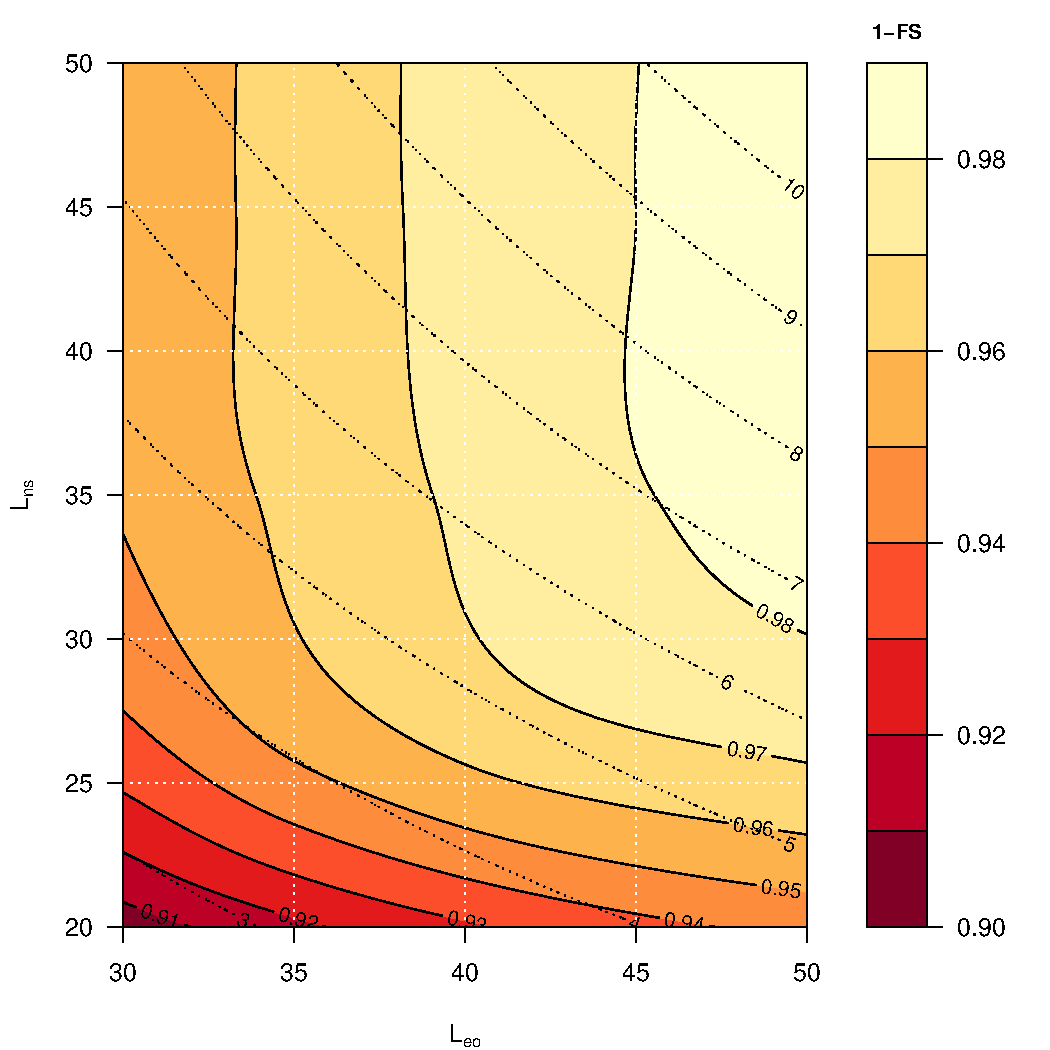
\includegraphics[height=0.4\textheight]{figuras/AbacoSombras.pdf}
\caption{Ábaco para planta de seguimiento a doble eje. Recoge el ratio entre la energía anual producida por un seguidor afectado por sombras mutuas (\(E_{acS}\)) y la producida por un seguidor sin sombreado (\(E_{ac0}\)). Las curvas de color negro representan la fracción de energía no afectada por sombras. Las curvas de puntos representan el valor del ROT. Figura 6.14 del libro ESF \cite{Perpinan2023}. \label{fig:abaco-sombras}}
\end{figure}

\subsection{Sistemas de seguimiento de eje horizontal}
\label{sec:orga637cc2}
Se considera que los seguidores son de longitud infinita en sentido Norte-Sur (se desprecia el efecto de borde). Así, los parámetros que determinan el diseño de este tipo de sistema son (figura \ref{fig:SeguidorEjeHorizontalSombras}):
\begin{figure}[htbp]
\centering
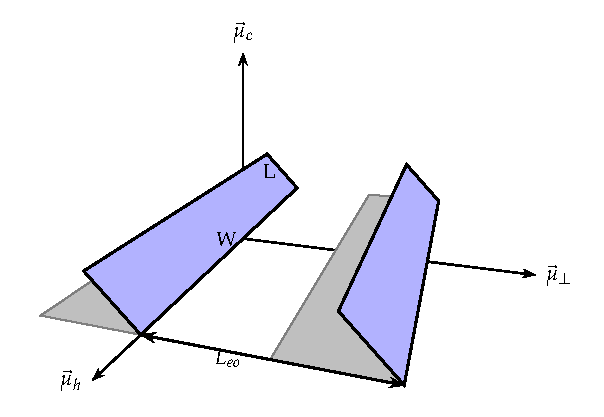
\includegraphics[scale=0.9]{figuras/SombrasHoriz.pdf}
\caption{Dimensiones básicas en sistemas con seguidores de eje horizontal. Figura 6.16 del libro ESF \cite{Perpinan2023}. \label{fig:SeguidorEjeHorizontalSombras}}
\end{figure}
\begin{enumerate}
\item La inclinación del generador fotovoltaico, \(\beta\), (coincidente con el ángulo \(\psi_{ns}\)).
\item La dimensión en sentido Este-Oeste del campo generador, L.
\item La separación entre los diferente seguidores en la dirección Este-Oeste, \(L_{eo}\).
Por tanto, \(ROT=\frac{L_{eo}}{L}\).
\end{enumerate}

Para caracterizar numéricamente el sombreado, se empreará el factor \(FS_{eo}\). Mediante consideraciones geométricas, utilizando la distancia normalizada \(l_{eo}=\frac{L_{eo}}{L}\), es posible escribir:
\begin{align}
FS_{eo} & =\frac{s-l_{eo}}{s}\nonumber \\
 & =1-l_{eo}\cdot\cos(\beta)\nonumber \\
 &
 =1-l_{eo}\cdot\frac{\sin(\omega)}{\sqrt{\sin^{2}(\omega)+\left(\cos(\omega)\cos(\phi)+\tan(\delta)\sin(\phi)\right)^{2}}}\label{eq:FSeoHorizontal}
\end{align}

\subsubsection{Limitación de ángulo y retroseguimeitno}
\label{sec:orge979f53}
En seguidores de eje horizontal se puede evitar la incidencia de sombras en cualquier en cualquier instante mediante algoritmos de \emph{backtracking} o retroseguimiento \cite{Panico.Garvison.ea1991}. Esta técnia provoca el desvío del seguidor de su posición óptima en los instantes en los que se produce la sombra entre seguidores, evitando el impacto de sombras pero con la consiguiente reducción en energía producida pro alejamiento del apuntamiento óptimo.

Para evitar la aparición de sombras, el ángulo de inclinación de los seguidores debe ser tal que la longitud de la sombra sea igual a la distancia entre seguidores. Siendo, \(\beta\) el ángulo de inclinación con retroseguimiento, y, \(\beta_0\) el ángulo de inclinación original, de la ecuación \ref{eq:FSeoHorizontal} se deduce que sólo será necesario aplicar esta técnica cuando \(l_{eo}\cdot cos(\beta_0) \leq 1\). El triángulo definido por el rayo solar, el seguidro y la sombra debe cumplir la siguiente condición, basada en el teorema de los senos:
\begin{equation}
\label{eq:BT_senos}
\frac{l_{eo}}{\cos(\beta_0-\beta)}=\frac{1}{\cos{\beta_0}}
\end{equation}

Por tanto, el ángulo de inclinación que grantiza la ausencia de sombras a costa de apartarse de la condición de seguimiento es:
\begin{equation}
\label{eq:retroseguimiento}
\beta=\beta_0-\arccos(l_{eo}\cdot\cos{\beta_0})  
\end{equation}
ecuación que debe aplicarse sólo cuando \(l_{eo} \cdot \cos(\beta_0) \leq 1\). En caso contrario \(\beta = \beta_0\).


\chapter{Desarrollo del código}
\label{chap:desarrollo-codigo}
En la figura \ref{fig:org6f4c4e3}, se muestra el proceso de cálculo que sigue el paquete a la hora de obtener la estimación de la producción del sistema fotovoltaico.
\begin{figure}[]
\centering
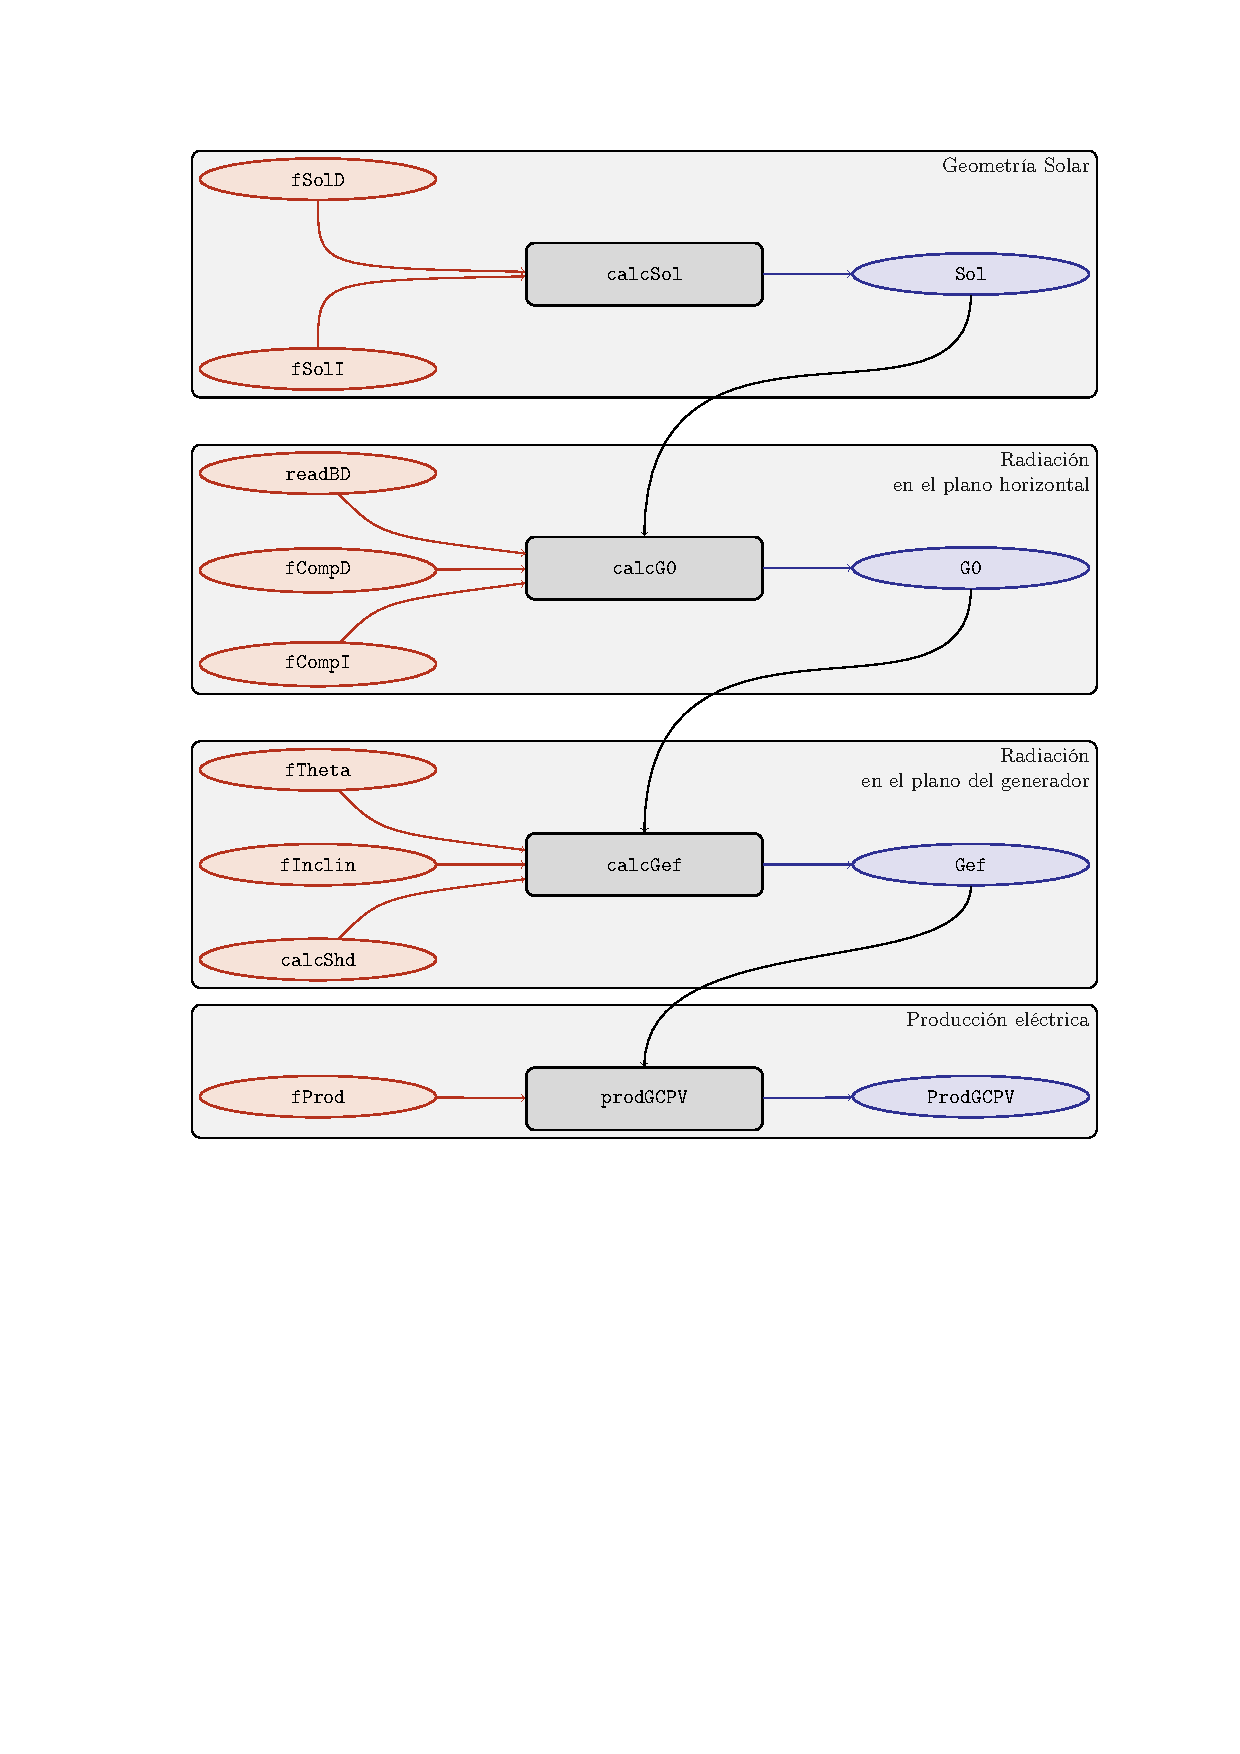
\includegraphics[keepaspectratio,width=0.8\textwidth,height=0.5\textheight]{figuras/procedure.pdf}
\caption{\label{fig:org6f4c4e3}Proceso de cálculo de las funciones de \texttt{solaR2}}
\end{figure}
A la hora de estimar la producción, el programa sigue los siguientes procesos:
\section{Geometría solar}
\label{sec:orgc775690}
\label{sec:geometria-solar}
Para calcular la geometría que definen las posiciones de la Tierra y el Sol, \texttt{solaR2} se vale de una función constructora, \texttt{calcSol} [\ref{subsec:calcsol}], la cual mediante las funciones \texttt{fSolD} [\ref{subsec:fsold}] y \texttt{fSolI} [\ref{subsec:fsoli}] cálcula todos los ángulos y componentes que caracterizan la geometría solar.
\begin{figure}[]
\centering
\includegraphics[keepaspectratio,width=\textwidth,height=0.5\textheight]{figuras/calcSol.pdf}
\caption{Cálculo de la geometría solar mediante la función \texttt{calcSol}, la cual unifica las funciones \texttt{fSolD} y \texttt{fSolI} resultando en un objeto clase \texttt{Sol} el cual contiene toda la información geométrica necesaria para realizar las siguientes estimaciones. \label{fig:calcSol}}
\end{figure}

Como se puede ver en la figura \ref{fig:calcSol}, \texttt{calcSol} funcia gracias a las siguientes funciones:
\begin{itemize}
\item \texttt{fSolD}: la cual, a partir de la latitud (\(\phi\)), computa la geometría a nivel diario, es decir, los ángulos y componentes que se pueden calcular en cada día independiente.

estas son:
\begin{itemize}
\item Declinación (\(\delta\)): calculada a partir de la función \texttt{declination}\footnote{Todas las funciones mencionadas en este punto, se encuentran en el apartado \ref{subsec:utils-angles}.}.
\item Excentricidad (\(\epsilon_o\)): obtenida mediante la función \texttt{eccentricity}.
\item Ecuación del tiempo (\(EoT\)): obtenida mediante la función \texttt{eot}.
\item Ángulo del amanecer (\(\omega_s\)): calculada a partir de la función \texttt{sunrise}.
\item Irradiancia diaria extra-atmosférica (\(B_{0d}(0)\)): obtenida a paritr de la función \texttt{bo0d}.
\end{itemize}
\end{itemize}
\begin{lstlisting}[numbers=left,language=r,label= ,caption= ,captionpos=b]
lat <- 37.2
BTd <- fBTd(mode = 'prom')
solD <- fSolD(lat = lat, BTd = BTd)
show(solD)
\end{lstlisting}

\begin{verbatim}
Key: <Dates>
         Dates   lat        decl        eo           EoT        ws      Bo0d
        <IDat> <num>       <num>     <num>         <num>     <num>     <num>
 1: 2024-01-17  37.2 -0.36271754 1.0340422 -0.0455346238 -1.278593  4738.993
 2: 2024-02-14  37.2 -0.22850166 1.0259717 -0.0614793356 -1.393341  6137.388
 3: 2024-03-15  37.2 -0.03191616 1.0107943 -0.0368674274 -1.546560  8086.323
 4: 2024-04-15  37.2  0.17531794 0.9926547  0.0017482721 -1.705659  9921.357
 5: 2024-05-15  37.2  0.33246485 0.9775162  0.0143055938 -1.835976 11115.619
 6: 2024-06-10  37.2  0.40257826 0.9691480 -0.0007378952 -1.899934 11573.907
 7: 2024-07-18  37.2  0.36439367 0.9675489 -0.0263454380 -1.864521 11257.133
 8: 2024-08-18  37.2  0.22407398 0.9758022 -0.0111761118 -1.744657 10183.208
 9: 2024-09-18  37.2  0.02730595 0.9907919  0.0342189964 -1.591529  8508.642
10: 2024-10-19  37.2 -0.17900474 1.0088406  0.0689613044 -1.433019  6554.218
11: 2024-11-18  37.2 -0.33862399 1.0245012  0.0575423573 -1.300179  4951.750
12: 2024-12-13  37.2 -0.40478283 1.0328516  0.0158622941 -1.239567  4284.472
\end{verbatim}

Además, \texttt{fSolD} permite seleccionar el método de cáculo entre los propuestos por 4 autores diferentes (\texttt{cooper} \cite{Cooper1969}, \texttt{spencer} \cite{Spencer1971}, \texttt{strous} \cite{Strous2011}, \texttt{michalsky} \cite{Michalsky1988})(el valor por defecto es \texttt{michalsky}):
\begin{lstlisting}[numbers=left,language=r,label= ,caption= ,captionpos=b]
solD_cooper <- fSolD(lat = lat, BTd = BTd, method = 'cooper')
show(solD_cooper)
\end{lstlisting}

\begin{verbatim}
Key: <Dates>
         Dates   lat        decl        eo           EoT        ws      Bo0d
        <IDat> <num>       <num>     <num>         <num>     <num>     <num>
 1: 2024-01-17  37.2 -0.36506987 1.0315970 -0.0455346238 -1.276457  4702.617
 2: 2024-02-14  37.2 -0.23770977 1.0235842 -0.0614793356 -1.385835  6024.833
 3: 2024-03-15  37.2 -0.04219743 1.0091112 -0.0368674274 -1.538742  7968.679
 4: 2024-04-15  37.2  0.17074888 0.9917107  0.0017482721 -1.702053  9870.335
 5: 2024-05-15  37.2  0.33214647 0.9770196  0.0143055938 -1.835696 11107.378
 6: 2024-06-10  37.2  0.40292516 0.9690335 -0.0007378952 -1.900263 11575.213
 7: 2024-07-18  37.2  0.36346384 0.9684861 -0.0263454380 -1.863677 11260.684
 8: 2024-08-18  37.2  0.21721704 0.9778484 -0.0111761118 -1.739110 10144.635
 9: 2024-09-18  37.2  0.01056696 0.9933706  0.0342189964 -1.578817  8367.014
10: 2024-10-19  37.2 -0.19902155 1.0107363  0.0689613044 -1.417100  6356.454
11: 2024-11-18  37.2 -0.34965673 1.0247443  0.0575423573 -1.290358  4835.353
12: 2024-12-13  37.2 -0.40651987 1.0315970  0.0158622941 -1.237915  4260.830
\end{verbatim}

\begin{lstlisting}[numbers=left,language=r,label= ,caption= ,captionpos=b]
solD_spencer <- fSolD(lat = lat, BTd = BTd, method = 'spencer')
show(solD_spencer)
\end{lstlisting}

\begin{verbatim}
Key: <Dates>
         Dates   lat        decl        eo           EoT        ws      Bo0d
        <IDat> <num>       <num>     <num>         <num>     <num>     <num>
 1: 2024-01-17  37.2 -0.36483670 1.0340422 -0.0455346238 -1.276669  4716.264
 2: 2024-02-14  37.2 -0.23199205 1.0259717 -0.0614793356 -1.390501  6100.057
 3: 2024-03-15  37.2 -0.03563921 1.0107943 -0.0368674274 -1.543730  8048.574
 4: 2024-04-15  37.2  0.17171286 0.9926547  0.0017482721 -1.702813  9888.522
 5: 2024-05-15  37.2  0.33007088 0.9775162  0.0143055938 -1.833871 11096.093
 6: 2024-06-10  37.2  0.40208757 0.9691480 -0.0007378952 -1.899469 11570.124
 7: 2024-07-18  37.2  0.36657157 0.9675489 -0.0263454380 -1.866501 11274.319
 8: 2024-08-18  37.2  0.22748717 0.9758022 -0.0111761118 -1.747427 10212.886
 9: 2024-09-18  37.2  0.03143967 0.9907919  0.0342189964 -1.594670  8548.821
10: 2024-10-19  37.2 -0.17549393 1.0088406  0.0689613044 -1.435795  6590.939
11: 2024-11-18  37.2 -0.33679169 1.0245012  0.0575423573 -1.301800  4971.285
12: 2024-12-13  37.2 -0.40419949 1.0328516  0.0158622941 -1.240121  4290.674
\end{verbatim}

\begin{lstlisting}[numbers=left,language=r,label= ,caption= ,captionpos=b]
solD_strous <- fSolD(lat = lat, BTd = BTd, method = 'cooper')
show(solD_strous)
\end{lstlisting}

\begin{verbatim}
Key: <Dates>
         Dates   lat        decl        eo           EoT        ws      Bo0d
        <IDat> <num>       <num>     <num>         <num>     <num>     <num>
 1: 2024-01-17  37.2 -0.36506987 1.0315970 -0.0455346238 -1.276457  4702.617
 2: 2024-02-14  37.2 -0.23770977 1.0235842 -0.0614793356 -1.385835  6024.833
 3: 2024-03-15  37.2 -0.04219743 1.0091112 -0.0368674274 -1.538742  7968.679
 4: 2024-04-15  37.2  0.17074888 0.9917107  0.0017482721 -1.702053  9870.335
 5: 2024-05-15  37.2  0.33214647 0.9770196  0.0143055938 -1.835696 11107.378
 6: 2024-06-10  37.2  0.40292516 0.9690335 -0.0007378952 -1.900263 11575.213
 7: 2024-07-18  37.2  0.36346384 0.9684861 -0.0263454380 -1.863677 11260.684
 8: 2024-08-18  37.2  0.21721704 0.9778484 -0.0111761118 -1.739110 10144.635
 9: 2024-09-18  37.2  0.01056696 0.9933706  0.0342189964 -1.578817  8367.014
10: 2024-10-19  37.2 -0.19902155 1.0107363  0.0689613044 -1.417100  6356.454
11: 2024-11-18  37.2 -0.34965673 1.0247443  0.0575423573 -1.290358  4835.353
12: 2024-12-13  37.2 -0.40651987 1.0315970  0.0158622941 -1.237915  4260.830
\end{verbatim}

\begin{itemize}
\item \texttt{fSolI}: toma los resultados obtenidos en \texttt{fSolD} y calcula la geometría a nivel intradiario, es decir, aquella que se puede calcular en unidades de tiempo menores a los días.
estas son:
\begin{itemize}
\item La hora solar o tiempo solar verdadero (\(\omega\)): calculada a partir de la función \texttt{sunHour}.
\item Los momentos del día en los que es de noche (\(night\)): calculada a partir del resultado anterior y de el ángulo del amanecer (cálculada en \texttt{fSolD})\footnote{Cuando la hora solar verdadera excede los ángulos en los que amanece y anochece (\(|\omega|>=|\omega_s|\)), el Sol queda por debajo de la línea del horizonte, por lo que es de noche.}.
\item El coseno del ángulo cenital solar (\(cos(\theta_{zs})\)): obtenida a partir de la función \texttt{zenith}.
\item La altura solar (\(\gamma_s\)): obtenida a partir del resultado anterior\footnote{\(\gamma_s=asin(cos(\theta_s))\).}.
\item El ángulo zenital solar (\(\theta_{zs}\)): calculada mediante la función \texttt{azimuth}.
\item La irradiancia extra-atmosférica (\(B_0(0)\)): calculada mediante el coseno del ángulo cenital, la constante solar (\(B_0\)) y la excentridad (cálculada en \texttt{fSolD}) [ecuación \ref{eq:irrad_horiz}].
\end{itemize}
\end{itemize}
\begin{lstlisting}[numbers=left,language=r,label= ,caption= ,captionpos=b]
solI <- fSolI(solD = solD[1], sample = 'hour') #Computo solo un día a fin mejorar la visualización
show(solI)
\end{lstlisting}

\begin{verbatim}
Index: <night>
                  Dates   lat           w  night      cosThzS          AlS         AzS       Bo0
                 <POSc> <num>       <num> <lgcl>        <num>        <num>       <num>     <num>
 1: 2024-01-17 00:00:00  37.2  3.09905026   TRUE -0.958552332 -1.281876984  3.00157749   0.00000
 2: 2024-01-17 01:00:00  37.2 -2.92239722   TRUE -0.941407376 -1.226779122 -2.49462689   0.00000
 3: 2024-01-17 02:00:00  37.2 -2.66065932   TRUE -0.874749489 -1.064918604 -2.03862388   0.00000
 4: 2024-01-17 03:00:00  37.2 -2.39892132   TRUE -0.763119126 -0.868125900 -1.77932134   0.00000
 5: 2024-01-17 04:00:00  37.2 -2.13718324   TRUE -0.614120126 -0.661270606 -1.59701536   0.00000
 6: 2024-01-17 05:00:00  37.2 -1.87544507   TRUE -0.437901763 -0.453263434 -1.44469585   0.00000
 7: 2024-01-17 06:00:00  37.2 -1.61370681   TRUE -0.246467423 -0.249033534 -1.30093496   0.00000
 8: 2024-01-17 07:00:00  37.2 -1.35196846   TRUE -0.052856976 -0.052881619 -1.15283370   0.00000
 9: 2024-01-17 08:00:00  37.2 -1.09023003  FALSE  0.129741461  0.130108233 -0.99014548 183.39419
10: 2024-01-17 09:00:00  37.2 -0.82849151  FALSE  0.288889848  0.293067041 -0.80329847 408.35612
11: 2024-01-17 10:00:00  37.2 -0.56675290  FALSE  0.413747472  0.426566560 -0.58400587 584.84684
12: 2024-01-17 11:00:00  37.2 -0.30501420  FALSE  0.495809380  0.518766586 -0.32921922 700.84427
13: 2024-01-17 12:00:00  37.2 -0.04327541  FALSE  0.529485721  0.557994217 -0.04769723 748.44699
14: 2024-01-17 13:00:00  37.2  0.21846346  FALSE  0.512482515  0.538073327  0.23821864 724.41235
15: 2024-01-17 14:00:00  37.2  0.48020243  FALSE  0.445957919  0.462244212  0.50355560 630.37745
16: 2024-01-17 15:00:00  37.2  0.74194148  FALSE  0.334443348  0.341014503  0.73469016 472.74762
17: 2024-01-17 16:00:00  37.2  1.00368062  FALSE  0.185534810  0.186616094  0.93148844 262.26008
18: 2024-01-17 17:00:00  37.2  1.26541985  FALSE  0.009375501  0.009375638  1.10112996  13.25261
19: 2024-01-17 18:00:00  37.2  1.52715917   TRUE -0.182035120 -0.183055757  1.25297092   0.00000
20: 2024-01-17 19:00:00  37.2  1.78889857   TRUE -0.375658695 -0.385107424  1.39694027   0.00000
21: 2024-01-17 20:00:00  37.2  2.05063807   TRUE -0.558306105 -0.592342658  1.54466726   0.00000
22: 2024-01-17 21:00:00  37.2  2.31237766   TRUE -0.717535874 -0.800258081  1.71368519   0.00000
23: 2024-01-17 22:00:00  37.2  2.57411733   TRUE -0.842501657 -1.001910427  1.93928567   0.00000
24: 2024-01-17 23:00:00  37.2  2.83585709   TRUE -0.924691065 -1.180223341  2.30977400   0.00000
                  Dates   lat           w  night      cosThzS          AlS         AzS       Bo0
\end{verbatim}

Además, como los datos nocturnos aportan poco a los cálculos que atañen a este proyecto, \texttt{fSolI} presenta la posibilidad de eliminar estos datos con el argumento \texttt{keep.night}.
\begin{lstlisting}[numbers=left,language=r,label= ,caption= ,captionpos=b]
solI_nigth <- fSolI(solD = solD[1], sample = 'hour', keep.night = FALSE)
show(solI_nigth)
\end{lstlisting}

\begin{verbatim}
                  Dates   lat           w  night     cosThzS         AlS         AzS       Bo0
                 <POSc> <num>       <num> <lgcl>       <num>       <num>       <num>     <num>
 1: 2024-01-17 08:00:00  37.2 -1.09023003  FALSE 0.129741461 0.130108233 -0.99014548 183.39419
 2: 2024-01-17 09:00:00  37.2 -0.82849151  FALSE 0.288889848 0.293067041 -0.80329847 408.35612
 3: 2024-01-17 10:00:00  37.2 -0.56675290  FALSE 0.413747472 0.426566560 -0.58400587 584.84684
 4: 2024-01-17 11:00:00  37.2 -0.30501420  FALSE 0.495809380 0.518766586 -0.32921922 700.84427
 5: 2024-01-17 12:00:00  37.2 -0.04327541  FALSE 0.529485721 0.557994217 -0.04769723 748.44699
 6: 2024-01-17 13:00:00  37.2  0.21846346  FALSE 0.512482515 0.538073327  0.23821864 724.41235
 7: 2024-01-17 14:00:00  37.2  0.48020243  FALSE 0.445957919 0.462244212  0.50355560 630.37745
 8: 2024-01-17 15:00:00  37.2  0.74194148  FALSE 0.334443348 0.341014503  0.73469016 472.74762
 9: 2024-01-17 16:00:00  37.2  1.00368062  FALSE 0.185534810 0.186616094  0.93148844 262.26008
10: 2024-01-17 17:00:00  37.2  1.26541985  FALSE 0.009375501 0.009375638  1.10112996  13.25261
\end{verbatim}

A parte, en vez de identificar el intervalo intradiario (con el argumento \texttt{sample}), se puede dar directamente la base temporal intradiaria.
\begin{lstlisting}[numbers=left,language=r,label= ,caption= ,captionpos=b]
BTi <- fBTi(BTd, sample = 'hour')
solI_BTi <- fSolI(solD, BTi = BTi)
show(solI_BTi)
\end{lstlisting}

\begin{verbatim}
Index: <night>
                   Dates   lat         w  night    cosThzS        AlS       AzS   Bo0
                  <POSc> <num>     <num> <lgcl>      <num>      <num>     <num> <num>
  1: 2024-01-17 00:00:00  37.2  3.099050   TRUE -0.9585523 -1.2818770  3.001577     0
  2: 2024-01-17 01:00:00  37.2 -2.922397   TRUE -0.9414074 -1.2267791 -2.494627     0
  3: 2024-01-17 02:00:00  37.2 -2.660659   TRUE -0.8747495 -1.0649186 -2.038624     0
  4: 2024-01-17 03:00:00  37.2 -2.398921   TRUE -0.7631191 -0.8681259 -1.779321     0
  5: 2024-01-17 04:00:00  37.2 -2.137183   TRUE -0.6141201 -0.6612706 -1.597015     0
 ---                                                                                 
284: 2024-12-13 19:00:00  37.2  1.856445   TRUE -0.4444110 -0.4605166  1.394524     0
285: 2024-12-13 20:00:00  37.2  2.118158   TRUE -0.6191456 -0.6676542  1.539641     0
286: 2024-12-13 21:00:00  37.2  2.379871   TRUE -0.7679298 -0.8756029  1.709361     0
287: 2024-12-13 22:00:00  37.2  2.641583   TRUE -0.8806309 -1.0771921  1.946876     0
288: 2024-12-13 23:00:00  37.2  2.903296   TRUE -0.9495736 -1.2518732  2.377338     0
\end{verbatim}

También, se puede indicar que no realice las correcciones de la ecuación del tiempo.
\begin{lstlisting}[numbers=left,language=r,label= ,caption= ,captionpos=b]
solI_EoT <- fSolI(solD = solD, BTi = BTi, EoT = FALSE)
show(solI_EoT)
\end{lstlisting}

\begin{verbatim}
Index: <night>
                   Dates   lat         w  night    cosThzS        AlS       AzS   Bo0
                  <POSc> <num>     <num> <lgcl>      <num>      <num>     <num> <num>
  1: 2024-01-17 00:00:00  37.2  3.099050   TRUE -0.9585523 -1.2818770  3.001577     0
  2: 2024-01-17 01:00:00  37.2 -2.922397   TRUE -0.9414074 -1.2267791 -2.494627     0
  3: 2024-01-17 02:00:00  37.2 -2.660659   TRUE -0.8747495 -1.0649186 -2.038624     0
  4: 2024-01-17 03:00:00  37.2 -2.398921   TRUE -0.7631191 -0.8681259 -1.779321     0
  5: 2024-01-17 04:00:00  37.2 -2.137183   TRUE -0.6141201 -0.6612706 -1.597015     0
 ---                                                                                 
284: 2024-12-13 19:00:00  37.2  1.856445   TRUE -0.4444110 -0.4605166  1.394524     0
285: 2024-12-13 20:00:00  37.2  2.118158   TRUE -0.6191456 -0.6676542  1.539641     0
286: 2024-12-13 21:00:00  37.2  2.379871   TRUE -0.7679298 -0.8756029  1.709361     0
287: 2024-12-13 22:00:00  37.2  2.641583   TRUE -0.8806309 -1.0771921  1.946876     0
288: 2024-12-13 23:00:00  37.2  2.903296   TRUE -0.9495736 -1.2518732  2.377338     0
\end{verbatim}

Finalmente, estas dos funciones, como se muestra en la figura \ref{fig:calcSol}, convergen en la función \texttt{calcSol}, dando como resultado un objeto de clase \texttt{Sol}. Este objeto muestra un sumario de ambos elementos junto con la latitud de los cálculos.
\begin{lstlisting}[numbers=left,language=r,label= ,caption= ,captionpos=b]
sol <- calcSol(lat = lat, BTd = BTd, sample = 'hour')
show(sol)
\end{lstlisting}

\begin{verbatim}
Object of class Sol 

Latitude:  37.2 degrees

Daily values:
     Dates                 decl                 eo              EoT                   ws        
 Min.   :2024-01-17   Min.   :-0.404783   Min.   :0.9675   Min.   :-0.0614793   Min.   :-1.900  
 1st Qu.:2024-04-07   1st Qu.:-0.256032   1st Qu.:0.9771   1st Qu.:-0.0289759   1st Qu.:-1.767  
 Median :2024-06-29   Median :-0.002305   Median :1.0007   Median : 0.0005052   Median :-1.569  
 Mean   :2024-07-01   Mean   :-0.001618   Mean   :1.0009   Mean   : 0.0008748   Mean   :-1.569  
 3rd Qu.:2024-09-25   3rd Qu.: 0.251172   3rd Qu.:1.0249   3rd Qu.: 0.0204515   3rd Qu.:-1.370  
 Max.   :2024-12-13   Max.   : 0.402578   Max.   :1.0340   Max.   : 0.0689613   Max.   :-1.240  
      Bo0d      
 Min.   : 4284  
 1st Qu.: 5841  
 Median : 8297  
 Mean   : 8109  
 3rd Qu.:10416  
 Max.   :11574  

Intradaily values: 
     Dates                           w                night            cosThzS          
 Min.   :2024-01-17 00:00:00   Min.   :-3.1393050   Mode :logical   Min.   :-0.9700256  
 1st Qu.:2024-04-07 11:45:00   1st Qu.:-1.5692285   FALSE:145       1st Qu.:-0.5004531  
 Median :2024-06-29 11:30:00   Median : 0.0010871   TRUE :143       Median : 0.0062923  
 Mean   :2024-07-01 15:30:00   Mean   : 0.0009975                   Mean   :-0.0009523  
 3rd Qu.:2024-09-26 11:15:00   3rd Qu.: 1.5716412                   3rd Qu.: 0.5007129  
 Max.   :2024-12-13 23:00:00   Max.   : 3.1413972                   Max.   : 0.9697262  
      AlS                 AzS                 Bo0          
 Min.   :-1.325336   Min.   :-3.139169   Min.   :   0.000  
 1st Qu.:-0.524130   1st Qu.:-1.570722   1st Qu.:   0.000  
 Median : 0.006292   Median : 0.003834   Median :   8.748  
 Mean   :-0.001202   Mean   : 0.001011   Mean   : 337.752  
 3rd Qu.: 0.524433   3rd Qu.: 1.555342   3rd Qu.: 698.153  
 Max.   : 1.324107   Max.   : 3.141331   Max.   :1284.718
\end{verbatim}

\section{Datos meteorológicos}
\label{sec:org5e25673}
\label{sec:datos-meteorologicos}
Para el procesamiento de datos meteorologicos, \texttt{solaR2} provee una serie de funciones\footnote{Las funciones comentadas en este apartado, se recogen en la sección \ref{subsec:meteoreaders}} que son capaces de leer todo tipo de datos. Estos datos se procesan y se almacenan en un objeto de tipo \texttt{Meteo} tal y como se ve en la figura \ref{fig:meteo}. Estas funciones son:
\begin{figure}[]
\centering
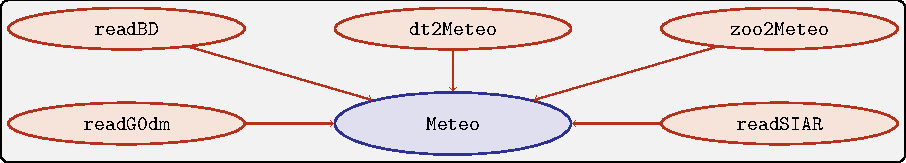
\includegraphics[keepaspectratio,width=\textwidth,height=0.5\textheight]{figuras/meteo.pdf}
\caption{Los datos meteorologicas se pueden leer mediante las funciones \texttt{readG0dm}, \texttt{readBD}, \texttt{dt2Meteo}, \texttt{zoo2Meteo} y \texttt{readSIAR} las cuales procesan estos datos y los almacenan en un objeto de clase \texttt{Meteo}. \label{fig:meteo}}
\end{figure}
\begin{itemize}
\item \texttt{readG0dm}: Esta función construye un objeto \texttt{Meteo} a partir de 12 valores de medias mensuales de irradiación.
\end{itemize}
\begin{lstlisting}[numbers=left,language=r,label= ,caption= ,captionpos=b]
G0dm = c(2.766,3.491,4.494,5.912,6.989,7.742,
         7.919,7.027,5.369,3.562,2.814,2.179) * 1000;
Ta = c(10, 14.1, 15.6, 17.2, 19.3, 21.2,
       28.4, 29.9, 24.3, 18.2, 17.2, 15.2)
BD <- readG0dm(G0dm = G0dm, Ta = Ta, lat = 37.2)
show(BD)
\end{lstlisting}

\begin{verbatim}
Object of class  Meteo 

Source of meteorological information: prom- 
Latitude of source:  37.2 degrees

Meteorological Data:
     Dates                 G0d             Ta       
 Min.   :2024-01-17   Min.   :2179   Min.   :10.00  
 1st Qu.:2024-04-07   1st Qu.:3322   1st Qu.:15.50  
 Median :2024-06-29   Median :4932   Median :17.70  
 Mean   :2024-07-01   Mean   :5022   Mean   :19.22  
 3rd Qu.:2024-09-25   3rd Qu.:6998   3rd Qu.:21.98  
 Max.   :2024-12-13   Max.   :7919   Max.   :29.90
\end{verbatim}

\begin{itemize}
\item \texttt{readBD}: Esta familia de funciones puede leer ficheros de datos y transformarlos en un objeto de clase \texttt{Meteo}. Se dividen en:
\begin{itemize}
\item \texttt{readBDd}: Procesa datos meteorológicos de tipo diarios.
\end{itemize}
\begin{lstlisting}[numbers=left,language=r,label= ,caption= ,captionpos=b]
## Se utiliza un archivo alojado en el
## github del tutor de este proyecto 
myURL <-"https://raw.githubusercontent.com/oscarperpinan/R/master/data/aranjuez.csv"
download.file(myURL, 'data/aranjuez.csv', quiet = TRUE)
BDd <- readBDd(file = 'data/aranjuez.csv', lat = lat,
               format = '%Y-%m-%d', header = TRUE,
               fill = TRUE, dec = '.', sep = ',', dates.col = '',
               ta.col = 'TempAvg', g0.col = 'Radiation', keep.cols = TRUE)
show(BDd)
\end{lstlisting}

\begin{verbatim}
Object of class  Meteo 

Source of meteorological information: bd-data/aranjuez.csv 
Latitude of source:  37.2 degrees

Meteorological Data:
     Dates                  G0               Ta            TempMin           TempMax      
 Min.   :2004-01-01   Min.   : 0.277   Min.   :-5.309   Min.   :-12.980   Min.   :-2.362  
 1st Qu.:2005-12-29   1st Qu.: 9.370   1st Qu.: 7.692   1st Qu.:  1.515   1st Qu.:14.530  
 Median :2008-01-09   Median :16.660   Median :13.810   Median :  7.170   Median :21.670  
 Mean   :2008-01-03   Mean   :16.742   Mean   :14.405   Mean   :  6.888   Mean   :22.531  
 3rd Qu.:2010-01-02   3rd Qu.:24.650   3rd Qu.:21.615   3rd Qu.: 12.590   3rd Qu.:30.875  
 Max.   :2011-12-31   Max.   :32.740   Max.   :30.680   Max.   : 22.710   Max.   :41.910  
		      NA's   :13                        NA's   :4                         
    HumidAvg         HumidMax         WindAvg         WindMax            Rain              ET       
 Min.   : 19.89   Min.   : 35.88   Min.   :0.251   Min.   : 0.000   Min.   : 0.000   Min.   :0.000  
 1st Qu.: 47.04   1st Qu.: 81.60   1st Qu.:0.667   1st Qu.: 3.783   1st Qu.: 0.000   1st Qu.:1.168  
 Median : 62.58   Median : 90.90   Median :0.920   Median : 5.027   Median : 0.000   Median :2.758  
 Mean   : 62.16   Mean   : 87.22   Mean   :1.174   Mean   : 5.208   Mean   : 1.094   Mean   :3.091  
 3rd Qu.: 77.38   3rd Qu.: 94.90   3rd Qu.:1.431   3rd Qu.: 6.537   3rd Qu.: 0.200   3rd Qu.:4.926  
 Max.   :100.00   Max.   :100.00   Max.   :8.260   Max.   :10.000   Max.   :49.730   Max.   :8.564  
		  NA's   :13       NA's   :8       NA's   :128      NA's   :4        NA's   :18
\end{verbatim}

\begin{itemize}
\item \texttt{readBDi}: Procesa datos meteorológicos de tipo intradiarios.
\end{itemize}
\begin{lstlisting}[numbers=left,language=r,label= ,caption= ,captionpos=b]
myURL <- "https://raw.githubusercontent.com/oscarperpinan/R/master/data/NREL-Hawaii.csv"
download.file(myURL, 'data/NREL-Hawaii.csv', quiet = TRUE)
BDi <- readBDi(file = 'data/NREL-Hawaii.csv', lat = 19,
               format = "%d/%m/%Y %H:%M", header = TRUE,
               fill = TRUE, dec = '.', sep = ',',
               dates.col = 'DATE', times.col = 'HST',
               ta.col = 'Air Temperature [deg C]',
               g0.col = 'Global Horizontal [W/m^2]',
               keep.cols = TRUE)
show(BDi)
\end{lstlisting}

\begin{verbatim}
Object of class  Meteo 

Source of meteorological information: bdI-data/NREL-Hawaii.csv 
Latitude of source:  19 degrees

Meteorological Data:
     Dates                              G0                  Ta        Direct Normal [W/m^2]
 Min.   :2010-01-11 06:32:00.00   Min.   :   0.4769   Min.   :13.42   Min.   :  0.0        
 1st Qu.:2010-03-11 17:37:45.00   1st Qu.: 147.4328   1st Qu.:22.76   1st Qu.:  0.0        
 Median :2010-06-11 17:32:30.00   Median : 300.6510   Median :24.15   Median :270.3        
 Mean   :2010-06-26 11:55:22.63   Mean   : 370.5293   Mean   :23.64   Mean   :356.6        
 3rd Qu.:2010-09-11 17:34:15.00   3rd Qu.: 585.7402   3rd Qu.:25.24   3rd Qu.:715.2        
 Max.   :2010-12-11 17:46:00.00   Max.   :1172.3000   Max.   :28.12   Max.   :943.0        
 NA's   :4660                                                                              
 Diffuse Horizontal [W/m^2]
 Min.   :  0.4769          
 1st Qu.: 78.4636          
 Median :152.9320          
 Mean   :171.7706          
 3rd Qu.:246.3193          
 Max.   :586.3600
\end{verbatim}

\item \texttt{dt2Meteo}: Transforma un \texttt{data.table} o \texttt{data.frame} en un objeto de clase \texttt{Meteo}.
\end{itemize}
\begin{lstlisting}[numbers=left,language=r,label= ,caption= ,captionpos=b]
data(helios)
names(helios) <- c('Dates', 'G0d', 'TempMax', 'TempMin')
helios_meteo <- dt2Meteo(file = helios, lat = 40, type = 'bd')
show(helios_meteo)
\end{lstlisting}

\begin{verbatim}
Object of class  Meteo 

Source of meteorological information: bd-data.frame 
Latitude of source:  40 degrees

Meteorological Data:
     Dates                             G0d             TempMin           TempMax     
 Min.   :2009-01-01 00:00:00.00   Min.   :  325.6   Min.   :-37.500   Min.   : 1.41  
 1st Qu.:2009-04-08 12:00:00.00   1st Qu.: 2523.2   1st Qu.:  1.950   1st Qu.:14.41  
 Median :2009-07-07 00:00:00.00   Median : 4745.7   Median :  7.910   Median :23.16  
 Mean   :2009-07-04 21:29:54.93   Mean   : 4812.0   Mean   :  5.323   Mean   :22.59  
 3rd Qu.:2009-10-03 12:00:00.00   3rd Qu.: 7139.5   3rd Qu.: 15.105   3rd Qu.:31.06  
 Max.   :2009-12-31 00:00:00.00   Max.   :11253.9   Max.   : 24.800   Max.   :38.04  
       Ta         
 Min.   :-23.049  
 1st Qu.:  7.008  
 Median : 12.055  
 Mean   : 10.944  
 3rd Qu.: 19.472  
 Max.   : 28.619
\end{verbatim}

\begin{itemize}
\item \texttt{zoo2Meteo}: Transforma un objeto de clase \texttt{zoo}\footnote{Pese a que este proyecto trate de ``desligarse'' del paquete \texttt{zoo}, sigue siendo un paquete muy extendido. Por lo que es interesante tener una función así para que los usuarios tengan una mayor flexibilidad.} en un objeto de clase \texttt{Meteo}.
\end{itemize}
\begin{lstlisting}[numbers=left,language=r,label= ,caption= ,captionpos=b]
library(zoo)
bd_zoo <- read.csv.zoo('data/aranjuez.csv')
BD_zoo <- zoo2Meteo(file = bd_zoo, lat = 40)
show(BD_zoo)
\end{lstlisting}

\begin{verbatim}
Object of class  Meteo 

Source of meteorological information: bd-zoo-bd_zoo 
Latitude of source:  40 degrees

Meteorological Data:
    TempAvg          TempMax          TempMin           HumidAvg         HumidMax         WindAvg     
 Min.   :-5.309   Min.   :-2.362   Min.   :-12.980   Min.   : 19.89   Min.   : 35.88   Min.   :0.251  
 1st Qu.: 7.692   1st Qu.:14.530   1st Qu.:  1.515   1st Qu.: 47.04   1st Qu.: 81.60   1st Qu.:0.667  
 Median :13.810   Median :21.670   Median :  7.170   Median : 62.58   Median : 90.90   Median :0.920  
 Mean   :14.405   Mean   :22.531   Mean   :  6.888   Mean   : 62.16   Mean   : 87.22   Mean   :1.174  
 3rd Qu.:21.615   3rd Qu.:30.875   3rd Qu.: 12.590   3rd Qu.: 77.38   3rd Qu.: 94.90   3rd Qu.:1.431  
 Max.   :30.680   Max.   :41.910   Max.   : 22.710   Max.   :100.00   Max.   :100.00   Max.   :8.260  
                                   NA's   :4                          NA's   :13       NA's   :8      
    WindMax            Rain          Radiation            ET       
 Min.   : 0.000   Min.   : 0.000   Min.   : 0.277   Min.   :0.000  
 1st Qu.: 3.783   1st Qu.: 0.000   1st Qu.: 9.370   1st Qu.:1.168  
 Median : 5.027   Median : 0.000   Median :16.660   Median :2.758  
 Mean   : 5.208   Mean   : 1.094   Mean   :16.742   Mean   :3.091  
 3rd Qu.: 6.537   3rd Qu.: 0.200   3rd Qu.:24.650   3rd Qu.:4.926  
 Max.   :10.000   Max.   :49.730   Max.   :32.740   Max.   :8.564  
 NA's   :128      NA's   :4        NA's   :13       NA's   :18
\end{verbatim}

\begin{itemize}
\item \texttt{readSIAR}: Esta función es capaz de extraer información de la red SIAR y transformarlo en un objeto de clase \texttt{Meteo}.
\end{itemize}
\begin{lstlisting}[numbers=left,language=r,label= ,caption= ,captionpos=b]
library(httr2)
library(jsonlite)
bd_SIAR <- readSIAR(Lat = 40.40596822621351, Lon = -3.70038308516172,
                    ## Ubicación de la Escuela Técnica Superior
                    ## de Ingeniería y Diseño Industrial (ETSIDI)
                    inicio = '2023-09-01', final = '2024-08-01',
                    tipo = 'Mensuales', n_est = 3)
show(bd_SIAR)
\end{lstlisting}

\begin{verbatim}
Object of class  Meteo 

Source of meteorological information: prom-https://servicio.mapama.gob.es 
  -Estaciones: Center: Finca experimental(M01), Arganda(M02), San Martín de la Vega(M05) 
Latitude of source:  40.4 degrees

Meteorological Data:
     Dates                          G0d             Ta            TempMin           TempMax     
 Min.   :2023-09-18 00:00:00   Min.   :1860   Min.   : 5.318   Min.   :-4.6513   Min.   :15.34  
 1st Qu.:2023-12-06 18:00:00   1st Qu.:2744   1st Qu.: 9.857   1st Qu.:-2.1466   1st Qu.:21.12  
 Median :2024-02-29 00:00:00   Median :4052   Median :14.890   Median : 0.3663   Median :31.01  
 Mean   :2024-03-01 04:00:00   Mean   :4529   Mean   :15.348   Mean   : 2.4225   Mean   :29.41  
 3rd Qu.:2024-05-21 12:00:00   3rd Qu.:6616   3rd Qu.:20.047   3rd Qu.: 7.1506   3rd Qu.:35.47  
 Max.   :2024-08-18 00:00:00   Max.   :7608   Max.   :27.560   Max.   :12.6082   Max.   :40.70
\end{verbatim}

Esta función tiene dos argumentos importantes:
\begin{itemize}
\item \texttt{tipo}: La API SIAR\footnote{La API (Interfaz de Programación de Aplicaciones) que se usa para la función \texttt{readSIAR} está proporcionada por la propia red SIAR \cite{siar23}.} permite tener 4 tipos de registros: \texttt{Mensuales}, \texttt{Semanales}, \texttt{Diarios} y \texttt{Horarios}.
\item \texttt{n\_est}: Con este argumento, la función es capaz de localizar el número seleccionado de estaciones más proximas a la ubicación dada, y obtener los datos individuales de cada una de ellas. Una vez obtenidos estos datos realiza una interpolación de distancia inversa ponderada (IDW) y entrega un solo resultado. Es importante añadir que la API SIAR tiene una limitación a la solicitud de registros que se le hace cada minuto, por lo que esta función cuenta con un comprobante para impedir que el usuario exceda este límite.
\end{itemize}

\section{Radiación en el plano horizontal}
\label{sec:org3b61c97}
\label{sec:radiacion-plano-horizontal}
Una vez se ha calculado la geometría solar (sección \ref{sec:geometria-solar}) y se han procesado los datos meteorológicos (sección \ref{sec:datos-meteorologicos}), es necesario calcular la radiación en el plano horizontal. Para ello, \texttt{solaR2} cuenta con la función \texttt{calcG0} [\ref{subsec:calcg0}] la cual mediante las funciones \texttt{fCompD} [\ref{subsec:fcompd}] y \texttt{fCompI} [\ref{subsec:fcompi}] procesan los objetos de clase \texttt{Sol} y clase \texttt{Meteo} para dar un objeto de tipo \texttt{G0}.

Como se puede ver en la figura \ref{fig:calcg0}, \texttt{calcG0} funciona gracias a las siguientes funciones:
\begin{figure}[]
\centering
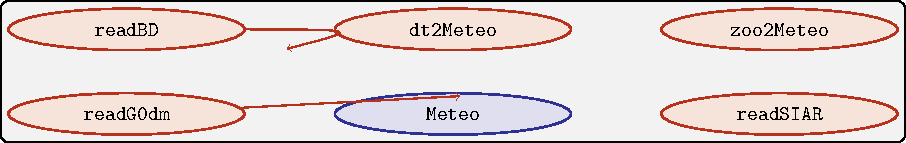
\includegraphics[keepaspectratio,width=\textwidth,height=0.5\textheight]{figuras/calcg0.pdf}
\caption{Cálculo de la radiación incidente en el plano horizontal mediante la función \texttt{calcG0}, la cual procesa un objeto clase \texttt{Sol} y otro clase \texttt{Meteo} mediante las funciones \texttt{fCompD} y \texttt{fCompI} resultando en un objeto clase \texttt{G0}. :\label{fig:calcg0}}
\end{figure}
\begin{itemize}
\item \texttt{fCompD}: La cual computa todas las componentes de la irradiación diaria en una superficie horizontal mediante regresiones entre los parámetros del índice de claridad y la fracción difusa.
Para ello se pueden usar varias correlaciones dependiendo del tipo de datos:
\begin{itemize}
\item Mensuales:
\end{itemize}
\begin{lstlisting}[numbers=left,language=r,label= ,caption= ,captionpos=b]
lat <- 37.2
BTd <- fBTd(mode = 'prom')
solD <- fSolD(lat, BTd)
G0d <- c(2.766,3.491,4.494,5.912,6.989,7.742,7.919,7.027,5.369,3.562,2.814,2.179) * 1000
compD_page <- fCompD(sol = solD, G0d = G0d, corr = "Page")
compD_page
\end{lstlisting}

\begin{verbatim}
Key: <Dates>
	 Dates        Fd        Kt   G0d      D0d      B0d
	<POSc>     <num>     <num> <num>    <num>    <num>
 1: 2024-01-17 0.3404548 0.5836683  2766  941.698 1824.302
 2: 2024-02-14 0.3572461 0.5688088  3491 1247.146 2243.854
 3: 2024-03-15 0.3719989 0.5557532  4494 1671.763 2822.237
 4: 2024-04-15 0.3266485 0.5958862  5912 1931.146 3980.854
 5: 2024-05-15 0.2895069 0.6287549  6989 2023.364 4965.636
 6: 2024-06-10 0.2441221 0.6689185  7742 1889.994 5852.006
 7: 2024-07-18 0.2050844 0.7034651  7919 1624.064 6294.936
 8: 2024-08-18 0.2202349 0.6900576  7027 1547.591 5479.409
 9: 2024-09-18 0.2869638 0.6310055  5369 1540.708 3828.292
10: 2024-10-19 0.3858825 0.5434669  3562 1374.513 2187.487
11: 2024-11-18 0.3578392 0.5682839  2814 1006.959 1807.041
12: 2024-12-13 0.4253038 0.5085807  2179  926.737 1252.263
\end{verbatim}

\begin{lstlisting}[numbers=left,language=r,label= ,caption= ,captionpos=b]
compD_lj <- fCompD(sol = solD, G0d = G0d, corr = "LJ")
compD_lj
\end{lstlisting}

\begin{verbatim}
Key: <Dates>
	 Dates        Fd        Kt   G0d       D0d      B0d
	<POSc>     <num>     <num> <num>     <num>    <num>
 1: 2024-01-17 0.3058193 0.5836683  2766  845.8961 1920.104
 2: 2024-02-14 0.3169470 0.5688088  3491 1106.4621 2384.538
 3: 2024-03-15 0.3268047 0.5557532  4494 1468.6603 3025.340
 4: 2024-04-15 0.2967018 0.5958862  5912 1754.1011 4157.899
 5: 2024-05-15 0.2720419 0.6287549  6989 1901.3006 5087.699
 6: 2024-06-10 0.2408700 0.6689185  7742 1864.8154 5877.185
 7: 2024-07-18 0.2152460 0.7034651  7919 1704.5331 6214.467
 8: 2024-08-18 0.2236251 0.6900576  7027 1571.4138 5455.586
 9: 2024-09-18 0.2703347 0.6310055  5369 1451.4268 3917.573
10: 2024-10-19 0.3361895 0.5434669  3562 1197.5071 2364.493
11: 2024-11-18 0.3173415 0.5682839  2814  892.9990 1921.001
12: 2024-12-13 0.3637158 0.5085807  2179  792.5367 1386.463
\end{verbatim}

\begin{itemize}
\item Diarios:
\end{itemize}
\begin{lstlisting}[numbers=left,language=r,label= ,caption= ,captionpos=b]
G0d <- readSIAR(Lat = 40.40596822621351, Lon =-3.70038308516172,
                inicio = '2024-07-15', final = '2024-08-01',
                tipo = 'Diarios', n_est = 3)
sol <- calcSol(lat, BTd = indexD(G0d))
compD_cpr <- fCompD(sol = sol, G0d = G0d, corr = "CPR")
compD_cpr
\end{lstlisting}

\begin{verbatim}
Key: <Dates>
	 Dates        Fd        Kt      G0d      D0d      B0d
	<POSc>     <num>     <num>    <num>    <num>    <num>
 1: 2024-07-15 0.2833125 0.6798139 7697.945 2180.924 5517.021
 2: 2024-07-16 0.2597185 0.7000272 7911.858 2054.856 5857.002
 3: 2024-07-17 0.2815044 0.6812283 7684.293 2163.163 5521.131
 4: 2024-07-18 0.6627754 0.4674993 5262.702 3487.989 1774.713
 5: 2024-07-19 0.2595844 0.7001561 7865.166 2041.675 5823.491
 6: 2024-07-20 0.2594075 0.7003266 7849.961 2036.339 5813.622
 7: 2024-07-21 0.2315068 0.7365959 8237.938 1907.138 6330.799
 8: 2024-07-22 0.2269337 0.7493438 8361.056 1897.406 6463.650
 9: 2024-07-23 0.2451723 0.7156288 7965.753 1952.982 6012.771
10: 2024-07-24 0.2620008 0.6978638 7748.845 2030.204 5718.641
11: 2024-07-25 0.2746548 0.6867564 7606.140 2089.063 5517.077
12: 2024-07-26 0.3320728 0.6462270 7138.548 2370.518 4768.030
13: 2024-07-27 0.3186769 0.6547900 7213.697 2298.839 4914.858
14: 2024-07-28 0.2767163 0.6850625 7526.355 2082.665 5443.689
15: 2024-07-29 0.6566999 0.4709412 5159.260 3388.086 1771.174
16: 2024-07-30 0.3185533 0.6548709 7153.359 2278.726 4874.633
17: 2024-07-31 0.2503814 0.7096003 7728.034 1934.956 5793.078
18: 2024-08-01 0.2428514 0.7185406 7801.435 1894.589 5906.846
\end{verbatim}

\begin{lstlisting}[numbers=left,language=r,label= ,caption= ,captionpos=b]
compD_ekdd <- fCompD(sol = sol, G0d = G0d, corr = 'EKDd')
compD_ekdd
\end{lstlisting}

\begin{verbatim}
Key: <Dates>
	 Dates    Fd        Kt      G0d      D0d   B0d
	<POSc> <num>     <num>    <num>    <num> <num>
 1: 2024-07-15     1 0.6798139 7697.945 7697.945     0
 2: 2024-07-16     1 0.7000272 7911.858 7911.858     0
 3: 2024-07-17     1 0.6812283 7684.293 7684.293     0
 4: 2024-07-18     1 0.4674993 5262.702 5262.702     0
 5: 2024-07-19     1 0.7001561 7865.166 7865.166     0
 6: 2024-07-20     1 0.7003266 7849.961 7849.961     0
 7: 2024-07-21     1 0.7365959 8237.938 8237.938     0
 8: 2024-07-22     1 0.7493438 8361.056 8361.056     0
 9: 2024-07-23     1 0.7156288 7965.753 7965.753     0
10: 2024-07-24     1 0.6978638 7748.845 7748.845     0
11: 2024-07-25     1 0.6867564 7606.140 7606.140     0
12: 2024-07-26     1 0.6462270 7138.548 7138.548     0
13: 2024-07-27     1 0.6547900 7213.697 7213.697     0
14: 2024-07-28     1 0.6850625 7526.355 7526.355     0
15: 2024-07-29     1 0.4709412 5159.260 5159.260     0
16: 2024-07-30     1 0.6548709 7153.359 7153.359     0
17: 2024-07-31     1 0.7096003 7728.034 7728.034     0
18: 2024-08-01     1 0.7185406 7801.435 7801.435     0
\end{verbatim}

\begin{lstlisting}[numbers=left,language=r,label= ,caption= ,captionpos=b]
compD_climedd <- fCompD(sol = sol, G0d = G0d, corr = 'CLIMEDd')
compD_climedd
\end{lstlisting}

\begin{verbatim}
Key: <Dates>
	 Dates        Fd        Kt      G0d      D0d      B0d
	<POSc>     <num>     <num>    <num>    <num>    <num>
 1: 2024-07-15 0.2724591 0.6798139 7697.945 2097.375 5600.570
 2: 2024-07-16 0.2455880 0.7000272 7911.858 1943.057 5968.801
 3: 2024-07-17 0.2705287 0.6812283 7684.293 2078.822 5605.472
 4: 2024-07-18 0.6086148 0.4674993 5262.702 3202.958 2059.744
 5: 2024-07-19 0.2454217 0.7001561 7865.166 1930.282 5934.884
 6: 2024-07-20 0.2452020 0.7003266 7849.961 1924.826 5925.135
 7: 2024-07-21 0.2013208 0.7365959 8237.938 1658.468 6579.470
 8: 2024-07-22 0.1873678 0.7493438 8361.056 1566.592 6794.463
 9: 2024-07-23 0.2259736 0.7156288 7965.753 1800.050 6165.703
10: 2024-07-24 0.2483878 0.6978638 7748.845 1924.718 5824.126
11: 2024-07-25 0.2630540 0.6867564 7606.140 2000.826 5605.314
12: 2024-07-26 0.3202837 0.6462270 7138.548 2286.361 4852.187
13: 2024-07-27 0.3077503 0.6547900 7213.697 2220.018 4993.679
14: 2024-07-28 0.2653324 0.6850625 7526.355 1996.986 5529.369
15: 2024-07-29 0.6029930 0.4709412 5159.260 3110.998 2048.263
16: 2024-07-30 0.3076331 0.6548709 7153.359 2200.610 4952.749
17: 2024-07-31 0.2334298 0.7096003 7728.034 1803.954 5924.080
18: 2024-08-01 0.2224291 0.7185406 7801.435 1735.266 6066.168
\end{verbatim}

También, se puede aportar una función de corrección propia.
\begin{lstlisting}[numbers=left,language=r,label= ,caption= ,captionpos=b]
f_corrd <- function(sol, G0d){
  ## Función CLIMEDd
    Kt <- Ktd(sol, G0d)
    Fd=(Kt<=0.13)*(0.952)+
    (Kt>0.13 & Kt<=0.8)*(0.868+1.335*Kt-5.782*Kt^2+3.721*Kt^3)+
      (Kt>0.8)*0.141
  return(data.table(Fd, Kt))
}
compD_user <- fCompD(sol = sol, G0d = G0d, corr = 'user', f = f_corrd)
compD_user
\end{lstlisting}

\begin{verbatim}
Key: <Dates>
	 Dates        Fd        Kt      G0d      D0d      B0d
	<POSc>     <num>     <num>    <num>    <num>    <num>
 1: 2024-07-15 0.2724591 0.6798139 7697.945 2097.375 5600.570
 2: 2024-07-16 0.2455880 0.7000272 7911.858 1943.057 5968.801
 3: 2024-07-17 0.2705287 0.6812283 7684.293 2078.822 5605.472
 4: 2024-07-18 0.6086148 0.4674993 5262.702 3202.958 2059.744
 5: 2024-07-19 0.2454217 0.7001561 7865.166 1930.282 5934.884
 6: 2024-07-20 0.2452020 0.7003266 7849.961 1924.826 5925.135
 7: 2024-07-21 0.2013208 0.7365959 8237.938 1658.468 6579.470
 8: 2024-07-22 0.1873678 0.7493438 8361.056 1566.592 6794.463
 9: 2024-07-23 0.2259736 0.7156288 7965.753 1800.050 6165.703
10: 2024-07-24 0.2483878 0.6978638 7748.845 1924.718 5824.126
11: 2024-07-25 0.2630540 0.6867564 7606.140 2000.826 5605.314
12: 2024-07-26 0.3202837 0.6462270 7138.548 2286.361 4852.187
13: 2024-07-27 0.3077503 0.6547900 7213.697 2220.018 4993.679
14: 2024-07-28 0.2653324 0.6850625 7526.355 1996.986 5529.369
15: 2024-07-29 0.6029930 0.4709412 5159.260 3110.998 2048.263
16: 2024-07-30 0.3076331 0.6548709 7153.359 2200.610 4952.749
17: 2024-07-31 0.2334298 0.7096003 7728.034 1803.954 5924.080
18: 2024-08-01 0.2224291 0.7185406 7801.435 1735.266 6066.168
\end{verbatim}

Por último, si \texttt{G0d} ya contiene todos los componentes, se puede especifica que no haga ninguna corrección.
\begin{lstlisting}[numbers=left,language=r,label= ,caption= ,captionpos=b]
compD_none <- fCompD(sol = sol, G0d = compD_user, corr = 'none')
compD_none
\end{lstlisting}

\begin{verbatim}
Key: <Dates>
	 Dates        Fd        Kt      G0d      D0d      B0d
	<POSc>     <num>     <num>    <num>    <num>    <num>
 1: 2024-07-15 0.2724591 0.6798139 7697.945 2097.375 5600.570
 2: 2024-07-16 0.2455880 0.7000272 7911.858 1943.057 5968.801
 3: 2024-07-17 0.2705287 0.6812283 7684.293 2078.822 5605.472
 4: 2024-07-18 0.6086148 0.4674993 5262.702 3202.958 2059.744
 5: 2024-07-19 0.2454217 0.7001561 7865.166 1930.282 5934.884
 6: 2024-07-20 0.2452020 0.7003266 7849.961 1924.826 5925.135
 7: 2024-07-21 0.2013208 0.7365959 8237.938 1658.468 6579.470
 8: 2024-07-22 0.1873678 0.7493438 8361.056 1566.592 6794.463
 9: 2024-07-23 0.2259736 0.7156288 7965.753 1800.050 6165.703
10: 2024-07-24 0.2483878 0.6978638 7748.845 1924.718 5824.126
11: 2024-07-25 0.2630540 0.6867564 7606.140 2000.826 5605.314
12: 2024-07-26 0.3202837 0.6462270 7138.548 2286.361 4852.187
13: 2024-07-27 0.3077503 0.6547900 7213.697 2220.018 4993.679
14: 2024-07-28 0.2653324 0.6850625 7526.355 1996.986 5529.369
15: 2024-07-29 0.6029930 0.4709412 5159.260 3110.998 2048.263
16: 2024-07-30 0.3076331 0.6548709 7153.359 2200.610 4952.749
17: 2024-07-31 0.2334298 0.7096003 7728.034 1803.954 5924.080
18: 2024-08-01 0.2224291 0.7185406 7801.435 1735.266 6066.168
\end{verbatim}

\item \texttt{fCompI}: calcula, en base a los valores de irradiación diaria, todas las componentes de irradiancia. Se vale de dos procedimientos en base al tipo de argumentos que toma:
\begin{itemize}
\item \texttt{compD}: Si recibe un \texttt{data.table} resultado de \texttt{fCompD}, computa las relaciones entre las componentes de irradiancia e irradiación de las componentes de difusa y global, obteniendo con ellas un perfil de irradiancias [\ref{sec:radiacion-superficies-inclinadas}] (las irradiancias global y difusa salen de estas relaciones, mientras que la directa surge por diferencia entre las dos).
\end{itemize}
\begin{lstlisting}[numbers=left,language=r,label= ,caption= ,captionpos=b]
sol <- calcSol(lat = 37.2, BTd = fBTd(mode = 'prom'),
               sample = 'hour', keep.night = FALSE)
G0d <- c(2.766,3.491,4.494,5.912,6.989,7.742,7.919,
          7.027,5.369,3.562,2.814,2.179) * 1000
compD <- fCompD(sol = sol, G0d = G0d, corr = 'CPR')
compI <- fCompI(sol = sol, compD = compD)
show(compI)
\end{lstlisting}

\begin{verbatim}
Key: <Dates>
		   Dates        Fd        Kt        G0        D0        B0
		  <POSc>     <num>     <num>     <num>     <num>     <num>
  1: 2024-01-17 08:00:00 0.5656199 0.4583592  84.06042  47.54625  36.40399
  2: 2024-01-17 09:00:00 0.4912826 0.5277148 215.49558 105.86922 109.51548
  3: 2024-01-17 10:00:00 0.4453619 0.5821268 340.45500 151.62569 188.82159
  4: 2024-01-17 11:00:00 0.4195854 0.6178887 433.04376 181.69885 251.45464
  5: 2024-01-17 12:00:00 0.4098508 0.6325646 473.44106 194.04019 279.57020
 ---                                                                      
141: 2024-12-13 12:00:00 0.5437347 0.5488870 382.71443 208.09513 174.85828
142: 2024-12-13 13:00:00 0.5556284 0.5371376 352.10710 195.64071 156.62669
143: 2024-12-13 14:00:00 0.5893861 0.5063725 276.60890 163.02945 113.57257
144: 2024-12-13 15:00:00 0.6506594 0.4586869 172.87432 112.48231  60.23704
145: 2024-12-13 16:00:00 0.7511394 0.3973283  63.15968  47.44173  15.57107
\end{verbatim}

\begin{itemize}
\item \texttt{G0I}: Este argumento recibe datos de irradiancia, para después, poder aplicar las correcciones indicadas en el argumento \texttt{corr}.
\end{itemize}
\begin{lstlisting}[numbers=left,language=r,label= ,caption= ,captionpos=b]
G0I <- compI$G0
compI_ekdh <- fCompI(sol = sol, G0I = G0I, corr = 'EKDh')
show(compI_ekdh)
\end{lstlisting}

\begin{verbatim}
Key: <Dates>
		   Dates        Fd        Kt        G0        D0        B0
		  <POSc>     <num>     <num>     <num>     <num>     <num>
  1: 2024-01-17 08:00:00 0.7417600 0.4583592  84.06042  62.35265  21.70776
  2: 2024-01-17 09:00:00 0.6000150 0.5277148 215.49558 129.30057  86.19500
  3: 2024-01-17 10:00:00 0.4791716 0.5821268 340.45500 163.13636 177.31865
  4: 2024-01-17 11:00:00 0.4004462 0.6178887 433.04376 173.41074 259.63302
  5: 2024-01-17 12:00:00 0.3692679 0.6325646 473.44106 174.82659 298.61447
 ---                                                                      
141: 2024-12-13 12:00:00 0.5533972 0.5488870 382.71443 211.79307 170.92135
142: 2024-12-13 13:00:00 0.5793829 0.5371376 352.10710 204.00484 148.10226
143: 2024-12-13 14:00:00 0.6457949 0.5063725 276.60890 178.63262  97.97628
144: 2024-12-13 15:00:00 0.7411461 0.4586869 172.87432 128.12512  44.74920
145: 2024-12-13 16:00:00 0.8439123 0.3973283  63.15968  53.30123   9.85845
\end{verbatim}

\begin{lstlisting}[numbers=left,language=r,label= ,caption= ,captionpos=b]
compI_brl <- fCompI(sol = sol, G0I = G0I, corr = 'BRL')
show(compI_brl)
\end{lstlisting}

\begin{verbatim}
Key: <Dates>
		   Dates        Fd        Kt        G0        D0        B0
		  <POSc>     <num>     <num>     <num>     <num>     <num>
  1: 2024-01-17 08:00:00 0.6573908 0.4583592  84.06042  55.26054  28.79987
  2: 2024-01-17 09:00:00 0.5624767 0.5277148 215.49558 121.21125  94.28433
  3: 2024-01-17 10:00:00 0.4845081 0.5821268 340.45500 164.95322 175.50179
  4: 2024-01-17 11:00:00 0.4333714 0.6178887 433.04376 187.66880 245.37496
  5: 2024-01-17 12:00:00 0.4120068 0.6325646 473.44106 195.06094 278.38012
 ---                                                                      
141: 2024-12-13 12:00:00 0.5776181 0.5488870 382.71443 221.06278 161.65164
142: 2024-12-13 13:00:00 0.5917966 0.5371376 352.10710 208.37580 143.73130
143: 2024-12-13 14:00:00 0.6306611 0.5063725 276.60890 174.44649 102.16241
144: 2024-12-13 15:00:00 0.6887448 0.4586869 172.87432 119.06629  53.80803
145: 2024-12-13 16:00:00 0.7561974 0.3973283  63.15968  47.76119  15.39849
\end{verbatim}

\begin{lstlisting}[numbers=left,language=r,label= ,caption= ,captionpos=b]
compI_climedh <- fCompI(sol = sol, G0I = G0I, corr = 'CLIMEDh')
show(compI_climedh)
\end{lstlisting}

\begin{verbatim}
Key: <Dates>
		   Dates        Fd        Kt        G0        D0        B0
		  <POSc>     <num>     <num>     <num>     <num>     <num>
  1: 2024-01-17 08:00:00 0.7093252 0.4583592  84.06042  59.62617  24.43424
  2: 2024-01-17 09:00:00 0.5818534 0.5277148 215.49558 125.38683  90.10875
  3: 2024-01-17 10:00:00 0.4782729 0.5821268 340.45500 162.83039 177.62462
  4: 2024-01-17 11:00:00 0.4110389 0.6178887 433.04376 177.99784 255.04592
  5: 2024-01-17 12:00:00 0.3840268 0.6325646 473.44106 181.81406 291.62701
 ---                                                                      
141: 2024-12-13 12:00:00 0.5416063 0.5488870 382.71443 207.28055 175.43387
142: 2024-12-13 13:00:00 0.5639749 0.5371376 352.10710 198.57956 153.52754
143: 2024-12-13 14:00:00 0.6220088 0.5063725 276.60890 172.05317 104.55573
144: 2024-12-13 15:00:00 0.7087489 0.4586869 172.87432 122.52448  50.34984
145: 2024-12-13 16:00:00 0.8099691 0.3973283  63.15968  51.15739  12.00229
\end{verbatim}

Como con \texttt{fCompD}, se puede añadir una función correctora propia.
\begin{lstlisting}[numbers=left,language=r,label= ,caption= ,captionpos=b]
f_corri <- function(sol, G0i){
  ## Función CLIMEDh
  Kt <- Kti(sol, G0i)
  Fd=(Kt<=0.21)*(0.995-0.081*Kt)+
    (Kt>0.21 & Kt<=0.76)*(0.724+2.738*Kt-8.32*Kt^2+4.967*Kt^3)+
    (Kt>0.76)*0.180
  return(data.table(Fd, Kt))
}
compI_user <- fCompI(sol = sol, G0I = G0I, corr = 'user', f = f_corri)
show(compI_user)
\end{lstlisting}

\begin{verbatim}
Key: <Dates>
		   Dates        Fd        Kt        G0        D0        B0
		  <POSc>     <num>     <num>     <num>     <num>     <num>
  1: 2024-01-17 08:00:00 0.7093252 0.4583592  84.06042  59.62617  24.43424
  2: 2024-01-17 09:00:00 0.5818534 0.5277148 215.49558 125.38683  90.10875
  3: 2024-01-17 10:00:00 0.4782729 0.5821268 340.45500 162.83039 177.62462
  4: 2024-01-17 11:00:00 0.4110389 0.6178887 433.04376 177.99784 255.04592
  5: 2024-01-17 12:00:00 0.3840268 0.6325646 473.44106 181.81406 291.62701
 ---                                                                      
141: 2024-12-13 12:00:00 0.5416063 0.5488870 382.71443 207.28055 175.43387
142: 2024-12-13 13:00:00 0.5639749 0.5371376 352.10710 198.57956 153.52754
143: 2024-12-13 14:00:00 0.6220088 0.5063725 276.60890 172.05317 104.55573
144: 2024-12-13 15:00:00 0.7087489 0.4586869 172.87432 122.52448  50.34984
145: 2024-12-13 16:00:00 0.8099691 0.3973283  63.15968  51.15739  12.00229
\end{verbatim}

Y además, se puede no añadir corrección.
\begin{lstlisting}[numbers=left,language=r,label= ,caption= ,captionpos=b]
G0I <- compI_user
compI_none <- fCompI(sol = sol, G0I = G0I, corr = 'none')
show(compI_none)
\end{lstlisting}

\begin{verbatim}
Key: <Dates>
		   Dates        Fd        Kt        G0        D0        B0
		  <POSc>     <num>     <num>     <num>     <num>     <num>
  1: 2024-01-17 08:00:00 0.7093252 0.4583592  84.06042  59.62617  24.43424
  2: 2024-01-17 09:00:00 0.5818534 0.5277148 215.49558 125.38683  90.10875
  3: 2024-01-17 10:00:00 0.4782729 0.5821268 340.45500 162.83039 177.62462
  4: 2024-01-17 11:00:00 0.4110389 0.6178887 433.04376 177.99784 255.04592
  5: 2024-01-17 12:00:00 0.3840268 0.6325646 473.44106 181.81406 291.62701
 ---                                                                      
141: 2024-12-13 12:00:00 0.5416063 0.5488870 382.71443 207.28055 175.43387
142: 2024-12-13 13:00:00 0.5639749 0.5371376 352.10710 198.57956 153.52754
143: 2024-12-13 14:00:00 0.6220088 0.5063725 276.60890 172.05317 104.55573
144: 2024-12-13 15:00:00 0.7087489 0.4586869 172.87432 122.52448  50.34984
145: 2024-12-13 16:00:00 0.8099691 0.3973283  63.15968  51.15739  12.00229
\end{verbatim}

Por útlimo, esta función incluye un argumento extra, \texttt{filterG0} que cuando su valor es \texttt{TRUE}, elimina todos aquellos valores de irradiancia que son mayores que la irradiancia extra-atmosfércia (ya que es incoherente que la irradiancia terrestre sea mayor que la extra-terrestre)
\end{itemize}

Estas dos funciones, como se muestra en la figura \ref{fig:calcg0}, convergen en la función constructora \texttt{calcG0}, dando como resultado un objeto de clase \texttt{G0}. Este objeto muestra la media mensual de la irradiación diaria y la irradiación anual. A parte incluye los resultados de \texttt{fCompD} y \texttt{fCompI} y los objetos \texttt{Sol} y \texttt{Meteo} de los que parte.

Como argumento más importante está \texttt{modeRad}, el cual selecciona el tipo de datos que introduce el usuario en el argumento \texttt{dataRad}. Estos son:
\begin{itemize}
\item Medias mensuales.
\begin{lstlisting}[numbers=left,language=r,label= ,caption= ,captionpos=b]
G0dm <- c(2.766, 3.491, 4.494, 5.912, 6.989, 7.742, 7.919,
          7.027, 5.369, 3.562, 2.814, 2.179) * 1000
Ta <- c(10, 14.1, 15.6, 17.2, 19.3, 21.2,
       28.4, 29.9, 24.3, 18.2, 17.2, 15.2)
prom <- data.table(G0dm, Ta) 
g0_prom <- calcG0(lat, modeRad = 'prom', dataRad = prom)
show(g0_prom)
\end{lstlisting}

\begin{verbatim}
Object of class  G0 

Source of meteorological information: prom- 

Latitude of source:  37.2 degrees
Latitude for calculations:  37.2 degrees

Monthly avarages:
	Dates   G0d      D0d      B0d
       <char> <num>    <num>    <num>
 1: Jan. 2024 2.766 0.941698 1.824302
 2: Feb. 2024 3.491 1.247146 2.243854
 3: Mar. 2024 4.494 1.671763 2.822237
 4: Apr. 2024 5.912 1.931146 3.980854
 5: May. 2024 6.989 2.023364 4.965636
 6: Jun. 2024 7.742 1.889994 5.852006
 7: Jul. 2024 7.919 1.624064 6.294936
 8: Aug. 2024 7.027 1.547591 5.479409
 9: Sep. 2024 5.369 1.540708 3.828292
10: Oct. 2024 3.562 1.374513 2.187487
11: Nov. 2024 2.814 1.006959 1.807041
12: Dec. 2024 2.179 0.926737 1.252263

Yearly values:
   Dates      G0d      D0d      B0d
   <int>    <num>    <num>    <num>
1:  2024 1839.365 540.6331 1298.732
\end{verbatim}

\item Generación de secuencias diarias mediante matrices de transición de Markov.
\begin{lstlisting}[numbers=left,language=r,label= ,caption= ,captionpos=b]
g0_aguiar <- calcG0(lat, modeRad = 'aguiar', dataRad = prom)
show(g0_aguiar)
\end{lstlisting}

\begin{verbatim}
Object of class  G0 

Source of meteorological information: bd-aguiar 

Latitude of source:  37.2 degrees
Latitude for calculations:  37.2 degrees

Monthly avarages:
	Dates   G0d      D0d      B0d
       <char> <num>    <num>    <num>
 1: Jan. 2024 2.766 1.077532 1.688468
 2: Feb. 2024 3.491 1.581116 1.909884
 3: Mar. 2024 4.494 1.911563 2.582437
 4: Apr. 2024 5.912 2.360930 3.551070
 5: May. 2024 6.989 2.330537 4.658463
 6: Jun. 2024 7.742 2.483961 5.258039
 7: Jul. 2024 7.919 2.194992 5.724008
 8: Aug. 2024 7.027 2.183376 4.843624
 9: Sep. 2024 5.369 1.868099 3.500901
10: Oct. 2024 3.562 1.659716 1.902284
11: Nov. 2024 2.814 1.207916 1.606084
12: Dec. 2024 2.179 1.078214 1.100786

Yearly values:
Key: <Dates>
   Dates      G0d      D0d      B0d
   <int>    <num>    <num>    <num>
1:  2024 1839.365 668.9934 1170.372
\end{verbatim}

\item Diarios.
\begin{lstlisting}[numbers=left,language=r,label= ,caption= ,captionpos=b]
bd <- g0_aguiar@G0D
g0_bd <- calcG0(lat, modeRad = 'bd', dataRad = bd)
show(g0_bd)
\end{lstlisting}

\begin{verbatim}
Object of class  G0 

Source of meteorological information: bd-data.table 

Latitude of source:  37.2 degrees
Latitude for calculations:  37.2 degrees

Monthly avarages:
	Dates   G0d      D0d      B0d
       <char> <num>    <num>    <num>
 1: Jan. 2024 2.766 1.077532 1.688468
 2: Feb. 2024 3.491 1.581116 1.909884
 3: Mar. 2024 4.494 1.911563 2.582437
 4: Apr. 2024 5.912 2.360930 3.551070
 5: May. 2024 6.989 2.330537 4.658463
 6: Jun. 2024 7.742 2.483961 5.258039
 7: Jul. 2024 7.919 2.194992 5.724008
 8: Aug. 2024 7.027 2.183376 4.843624
 9: Sep. 2024 5.369 1.868099 3.500901
10: Oct. 2024 3.562 1.659716 1.902284
11: Nov. 2024 2.814 1.207916 1.606084
12: Dec. 2024 2.179 1.078214 1.100786

Yearly values:
Key: <Dates>
   Dates      G0d      D0d      B0d
   <int>    <num>    <num>    <num>
1:  2024 1839.365 668.9934 1170.372
\end{verbatim}

\item Intradiarios
\begin{lstlisting}[numbers=left,language=r,label= ,caption= ,captionpos=b]
bdI <- g0_aguiar@G0I
g0_bdI <- calcG0(lat, modeRad = 'bdI', dataRad = bdI)
show(g0_bdI)
\end{lstlisting}

\begin{verbatim}
Object of class  G0 

Source of meteorological information: bdI-data.table 

Latitude of source:  37.2 degrees
Latitude for calculations:  37.2 degrees

Monthly avarages:
	Dates      G0d      D0d      B0d
       <char>    <num>    <num>    <num>
 1: Jan. 2024 2.766000 1.014495 1.751505
 2: Feb. 2024 3.491000 1.584376 1.906624
 3: Mar. 2024 4.494000 2.002068 2.491932
 4: Apr. 2024 5.870393 2.367717 3.502676
 5: May. 2024 6.748807 1.946976 4.801831
 6: Jun. 2024 7.742000 2.476266 5.265734
 7: Jul. 2024 7.919000 1.778018 6.140982
 8: Aug. 2024 7.027000 1.834311 5.192689
 9: Sep. 2024 5.369000 1.787165 3.581835
10: Oct. 2024 3.562000 1.745649 1.816351
11: Nov. 2024 2.814000 1.223991 1.590009
12: Dec. 2024 2.179000 1.142758 1.036242

Yearly values:
Key: <Dates>
   Dates      G0d      D0d      B0d
   <int>    <num>    <num>    <num>
1:  2024 1830.671 636.9936 1193.677
\end{verbatim}
\end{itemize}

\section{Radiación efectiva en el plano del generador}
\label{sec:org45b7193}
\label{sec:radiacion-efectiva-plano-generador}
Teniendo la radiación incidente en plano horizontal (sección \ref{sec:radiacion-plano-horizontal}), se puede calcular la radiación efectiva incidente en el plano del generador. Para ello, \texttt{solaR2} cuenta con la función \texttt{calcGef} [\ref{subsec:calcgef}] la cual mediante las funciones \texttt{fInclin} y \texttt{calcShd} procesa un objeto de clase \texttt{G0} para obtener un objeto \texttt{Gef}.

Como se puede ver en la figura \ref{fig:calcgef}, \texttt{calcGef} funciona gracias a las siguientes funciones:
\begin{figure}[]
\centering
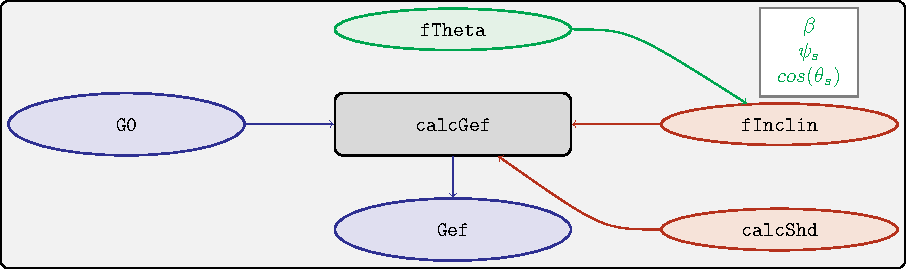
\includegraphics[keepaspectratio,width=\textwidth,height=0.5\textheight]{figuras/calcgef.pdf}
\caption{Cálculo de la radiación efectiva incidente en el plano del generador mediante la función \texttt{calcGef}, la cual emplea la función \texttt{fInclin} para el computo de las componentes efectivas, la función \texttt{fTheta} que provee a la función anterior los ángulos necesarios para su computo y la función \texttt{calcShd} que reprocesa el objeto de clase \texttt{Gef} resultante, añadiendole el efecto de las sombras producidas entres módulos. \label{fig:calcgef}}
\end{figure}
\begin{itemize}
\item \texttt{fTheta}: la cual, partiendo del ángulo de inclinación (\(\beta\)) y la orientación (\(\alpha\)), computa el ángulo de inclinación en cada instante (\(\beta\)), el ángulo azimutal (\(\psi_s\)) y el coseno del ángulo de incidencia  de la radiación solar en la superficie (\(cos(\theta_s)\)).
Como principal argumento tiene \texttt{modeTrk}, el cual determina el sistema de seguimiento que tiene el sistema:
\begin{itemize}
\item \texttt{fixed}: para sistemas estáticos.
\end{itemize}
\begin{lstlisting}[numbers=left,language=r,label= ,caption= ,captionpos=b]
BTd <- fBTd(mode = 'prom')[6] 
sol <- calcSol(lat, BTd = BTd, keep.night = FALSE)
beta <- lat - 10
alfa <- 0
angGen_fixed <- fTheta(sol = sol, beta = beta, alfa = alfa,
                 modeTrk = 'fixed')
show(angGen_fixed)
\end{lstlisting}

\begin{verbatim}
		  Dates      Beta  Alfa   cosTheta
		 <POSc>     <num> <num>      <num>
 1: 2024-06-10 05:00:00 0.4747296     0 0.00000000
 2: 2024-06-10 06:00:00 0.4747296     0 0.06990810
 3: 2024-06-10 07:00:00 0.4747296     0 0.30432148
 4: 2024-06-10 08:00:00 0.4747296     0 0.52263672
 5: 2024-06-10 09:00:00 0.4747296     0 0.70998013
 6: 2024-06-10 10:00:00 0.4747296     0 0.85358815
 7: 2024-06-10 11:00:00 0.4747296     0 0.94367686
 8: 2024-06-10 12:00:00 0.4747296     0 0.97410861
 9: 2024-06-10 13:00:00 0.4747296     0 0.94281011
10: 2024-06-10 14:00:00 0.4747296     0 0.85191372
11: 2024-06-10 15:00:00 0.4747296     0 0.70761218
12: 2024-06-10 16:00:00 0.4747296     0 0.51973665
13: 2024-06-10 17:00:00 0.4747296     0 0.30108697
14: 2024-06-10 18:00:00 0.4747296     0 0.06655958
15: 2024-06-10 19:00:00 0.4747296     0 0.00000000
\end{verbatim}

\begin{itemize}
\item \texttt{two}: para sistemas de seguimiento de doble eje.
\end{itemize}
\begin{lstlisting}[numbers=left,language=r,label= ,caption= ,captionpos=b]
angGen_two <- fTheta(sol = sol, beta = beta, alfa = alfa,
                     modeTrk = 'two')
show(angGen_two)
\end{lstlisting}

\begin{verbatim}
		  Dates      Beta         Alfa cosTheta
		 <POSc>     <num>        <num>    <num>
 1: 2024-06-10 05:00:00 1.5220852 -2.043678875        1
 2: 2024-06-10 06:00:00 1.3300857 -1.896688029        1
 3: 2024-06-10 07:00:00 1.1285281 -1.756655282        1
 4: 2024-06-10 08:00:00 0.9215732 -1.612213267        1
 5: 2024-06-10 09:00:00 0.7134716 -1.445120762        1
 6: 2024-06-10 10:00:00 0.5110180 -1.215351693        1
 7: 2024-06-10 11:00:00 0.3328578 -0.809087856        1
 8: 2024-06-10 12:00:00 0.2466893  0.006963841        1
 9: 2024-06-10 13:00:00 0.3349967  0.817155564        1
10: 2024-06-10 14:00:00 0.5137803  1.219398208        1
11: 2024-06-10 15:00:00 0.7163931  1.447776194        1
12: 2024-06-10 16:00:00 0.9245147  1.614353339        1
13: 2024-06-10 17:00:00 1.1314208  1.758631827        1
14: 2024-06-10 18:00:00 1.3328735  1.898691776        1
15: 2024-06-10 19:00:00 1.5247042  2.045849315        1
\end{verbatim}

\begin{itemize}
\item \texttt{horiz}: para sistemas de seguimiento horizontal Norte-Sur.
\end{itemize}
\begin{lstlisting}[numbers=left,language=r,label= ,caption= ,captionpos=b]
angGen_horiz <- fTheta(sol = sol, beta = beta, alfa = alfa,
                       modeTrk = 'horiz')
show(angGen_horiz)
\end{lstlisting}

\begin{verbatim}
		  Dates        Beta      Alfa  cosTheta
		 <POSc>       <num>     <num>     <num>
 1: 2024-06-10 05:00:00 1.516091993 -1.570796 0.8905353
 2: 2024-06-10 06:00:00 1.317263961 -1.570796 0.9504350
 3: 2024-06-10 07:00:00 1.121771495 -1.570796 0.9859551
 4: 2024-06-10 08:00:00 0.921160041 -1.570796 0.9994560
 5: 2024-06-10 09:00:00 0.709555740 -1.570796 0.9966296
 6: 2024-06-10 10:00:00 0.483954771 -1.570796 0.9854098
 7: 2024-06-10 11:00:00 0.245151627 -1.570796 0.9742418
 8: 2024-06-10 12:00:00 0.001753607  1.570796 0.9697277
 9: 2024-06-10 13:00:00 0.248597042  1.570796 0.9743648
10: 2024-06-10 14:00:00 0.487239436  1.570796 0.9855868
11: 2024-06-10 15:00:00 0.712638107  1.570796 0.9967482
12: 2024-06-10 16:00:00 0.924058412  1.570796 0.9993956
13: 2024-06-10 17:00:00 1.124550569  1.570796 0.9856166
14: 2024-06-10 18:00:00 1.320024608  1.570796 0.9497600
15: 2024-06-10 19:00:00 1.518974473  1.570796 0.8895182
\end{verbatim}

También, tiene un argumento \texttt{BT} que indica cuando se usa la técnica de backtracking para un sistema horizontal Norte-Sur. Para funcionar, necesita de los argumentos \texttt{struct}, el cual presenta una lista con la altura de los módulos, y \texttt{dist}, el cual presenta un \texttt{data.frame} (o \texttt{data.table}) con la distancia que separa los módulos en la dirección Este-Oeste.
\begin{lstlisting}[numbers=left,language=r,label= ,caption= ,captionpos=b]
struct <- list(L = 1)
distances <- data.table(Lew = 2)
angGen_BT <- fTheta(sol = sol, beta = beta, alfa = alfa,
                    modeTrk = 'horiz', BT = TRUE,
                    struct = struct, dist = distances)
show(angGen_BT)
\end{lstlisting}

\begin{verbatim}
		  Dates        Beta      Alfa   cosTheta
		 <POSc>       <num>     <num>      <num>
 1: 2024-06-10 05:00:00 0.054868903 -1.570796 0.09738369
 2: 2024-06-10 06:00:00 0.271972628 -1.570796 0.47678565
 3: 2024-06-10 07:00:00 0.602487004 -1.570796 0.85598103
 4: 2024-06-10 08:00:00 0.921160041 -1.570796 0.99945597
 5: 2024-06-10 09:00:00 0.709555740 -1.570796 0.99662956
 6: 2024-06-10 10:00:00 0.483954771 -1.570796 0.98540983
 7: 2024-06-10 11:00:00 0.245151627 -1.570796 0.97424175
 8: 2024-06-10 12:00:00 0.001753607  1.570796 0.96972767
 9: 2024-06-10 13:00:00 0.248597042  1.570796 0.97436477
10: 2024-06-10 14:00:00 0.487239436  1.570796 0.98558683
11: 2024-06-10 15:00:00 0.712638107  1.570796 0.99674816
12: 2024-06-10 16:00:00 0.924058412  1.570796 0.99939563
13: 2024-06-10 17:00:00 0.595256963  1.570796 0.85074877
14: 2024-06-10 18:00:00 0.268563625  1.570796 0.47136897
15: 2024-06-10 19:00:00 0.051961679  1.570796 0.09215170
\end{verbatim}

\item \texttt{fInclin}: la cual, partiendo del resultado de \texttt{fTheta} y de un objeto de clase \texttt{G0}, cálcula la irradiancia solar incidente en una superficie inclinada junto con los efectos del ángulo de incidencia y la suciedad para obtener la irradiancia efectiva.
Como argumentos principales están:
\begin{itemize}
\item \texttt{iS}: permite seleccionar entre 4 valores del 1 al 4 correspondientes al grado de suciedad del módulo. Siendo 1 limpio y 4 alto y basandose en los valores de la tabla \ref{tab:coef-perd} computa la irradiancia efectiva. Por defecto tiene valor 2 (grado de suciedad bajo).
\end{itemize}
\begin{lstlisting}[numbers=left,language=r,label= ,caption= ,captionpos=b]
compI <- calcG0(lat, dataRad = prom, keep.night = FALSE)
sol <- calcSol(lat, BTi = indexI(compI))
angGen <- fTheta(sol = sol, beta = beta, alfa = alfa)
inclin_limpio <- fInclin(compI = compI, angGen = angGen, iS = 1)
show(inclin_limpio)
\end{lstlisting}

\begin{verbatim}
		   Dates        Bo       Bn        G         D       Di        Dc         B         R
		  <POSc>     <num>    <num>    <num>     <num>    <num>     <num>     <num>     <num>
  1: 2024-01-17 08:00:00  514.5612 365.8727 186.4590  52.34286 25.82073  26.52212 133.18653 0.9295706
  2: 2024-01-17 09:00:00  792.6980 464.2106 366.6704 103.96230 52.12242  51.83988 260.32510 2.3830282
  3: 2024-01-17 10:00:00 1010.9063 541.3602 536.6247 145.69981 68.60264  77.09717 387.15997 3.7648749
  4: 2024-01-17 11:00:00 1154.3223 592.0663 662.0048 173.72247 77.44190  96.28057 483.49354 4.7887550
  5: 2024-01-17 12:00:00 1213.1770 612.8750 716.5974 185.35767 80.61172 104.74595 526.00427 5.2354830
 ---                                                                                                 
141: 2024-12-13 12:00:00 1181.1554 470.2512 578.4583 180.82966 95.85462  84.97504 393.39650 4.2321949
142: 2024-12-13 13:00:00 1129.5610 453.5904 536.8668 170.08970 91.70559  78.38411 362.88341 3.8937280
143: 2024-12-13 14:00:00  994.4636 409.9651 434.0673 142.25355 79.88147  62.37208 288.75488 3.0588416
144: 2024-12-13 15:00:00  785.0640 342.3463 292.1950  99.92831 58.81096  41.11735 190.35496 1.9117069
145: 2024-12-13 16:00:00  515.6229 255.3390 140.8937  46.94651 26.80445  20.14206  93.24874 0.6984426
	     FTb        FTd       FTr     Dief      Dcef      Gef       Def       Bef       Ref
	   <num>      <num>     <num>    <num>     <num>    <num>     <num>     <num>     <num>
  1: 0.115032290 0.05043622 0.2503398 24.51843  23.47122 166.5523  47.98966 117.86578 0.6968621
  2: 0.034235799 0.05043622 0.2503398 49.49356  50.06510 352.7578  99.55866 251.41266 1.7864615
  3: 0.012139104 0.05043622 0.2503398 65.14258  76.16128 526.5864 141.30386 382.46020 2.8223770
  4: 0.005426675 0.05043622 0.2503398 73.53602  95.75809 653.7538 169.29411 480.86978 3.5899392
  5: 0.003640433 0.05043622 0.2503398 76.54597 104.36463 708.9248 180.91060 524.08939 3.9248333
 ---                                                                                           
141: 0.004516349 0.05043622 0.2503398 91.02007  84.59127 570.4038 175.61134 391.61978 3.1727082
142: 0.006269898 0.05043622 0.2503398 87.08031  77.89265 528.5001 164.97296 360.60816 2.9189730
143: 0.013120704 0.05043622 0.2503398 75.85255  61.55372 424.6656 137.40626 284.96622 2.2930919
144: 0.035287438 0.05043622 0.2503398 55.84476  39.66642 280.5821  95.51118 183.63782 1.4331306
145: 0.114223038 0.05043622 0.2503398 25.45254  17.84137 126.4151  43.29391  82.59758 0.5235947
\end{verbatim}

\begin{lstlisting}[numbers=left,language=r,label= ,caption= ,captionpos=b]
inclin_sucio <- fInclin(compI = compI, angGen = angGen, iS = 4)
show(inclin_sucio)
\end{lstlisting}

\begin{verbatim}
		   Dates        Bo       Bn        G         D       Di        Dc         B         R
		  <POSc>     <num>    <num>    <num>     <num>    <num>     <num>     <num>     <num>
  1: 2024-01-17 08:00:00  514.5612 365.8727 186.4590  52.34286 25.82073  26.52212 133.18653 0.9295706
  2: 2024-01-17 09:00:00  792.6980 464.2106 366.6704 103.96230 52.12242  51.83988 260.32510 2.3830282
  3: 2024-01-17 10:00:00 1010.9063 541.3602 536.6247 145.69981 68.60264  77.09717 387.15997 3.7648749
  4: 2024-01-17 11:00:00 1154.3223 592.0663 662.0048 173.72247 77.44190  96.28057 483.49354 4.7887550
  5: 2024-01-17 12:00:00 1213.1770 612.8750 716.5974 185.35767 80.61172 104.74595 526.00427 5.2354830
 ---                                                                                                 
141: 2024-12-13 12:00:00 1181.1554 470.2512 578.4583 180.82966 95.85462  84.97504 393.39650 4.2321949
142: 2024-12-13 13:00:00 1129.5610 453.5904 536.8668 170.08970 91.70559  78.38411 362.88341 3.8937280
143: 2024-12-13 14:00:00  994.4636 409.9651 434.0673 142.25355 79.88147  62.37208 288.75488 3.0588416
144: 2024-12-13 15:00:00  785.0640 342.3463 292.1950  99.92831 58.81096  41.11735 190.35496 1.9117069
145: 2024-12-13 16:00:00  515.6229 255.3390 140.8937  46.94651 26.80445  20.14206  93.24874 0.6984426
	    FTb        FTd       FTr     Dief     Dcef      Gef       Def       Bef       Ref
	  <num>      <num>     <num>    <num>    <num>    <num>     <num>     <num>     <num>
  1: 0.24100175 0.09714708 0.3918962 21.44734 18.51982 133.4885  39.96716  93.00127 0.5200533
  2: 0.10321543 0.09714708 0.3918962 43.29416 42.77007 302.1765  86.06424 214.77909 1.3331982
  3: 0.04727214 0.09714708 0.3918962 56.98305 67.57641 466.0152 124.55946 339.34944 2.1062799
  4: 0.02455379 0.09714708 0.3918962 64.32515 86.40320 587.2996 150.72835 433.89218 2.6790952
  5: 0.01743586 0.09714708 0.3918962 66.95809 94.68605 640.0594 161.64413 475.48630 2.9290196
 ---                                                                                         
141: 0.02100686 0.09714708 0.3918962 79.61921 76.53478 512.8436 156.15400 354.32187 2.3677246
142: 0.02771140 0.09714708 0.3918962 76.17293 70.11502 473.0675 146.28795 324.60121 2.1783674
143: 0.05023795 0.09714708 0.3918962 66.35152 54.49955 374.8709 120.85106 252.30856 1.7112857
144: 0.10550059 0.09714708 0.3918962 48.84983 33.83709 240.4070  82.68692 156.65061 1.0695149
145: 0.23984890 0.09714708 0.3918962 22.26444 14.08613 101.9538  36.35057  65.21248 0.3907476
\end{verbatim}

\begin{itemize}
\item \texttt{alb} Correspondiente al coeficiente de reflexión del terreno para la irradiancia de albedo. Por defecto tiene un valor de 0,2 (valor aceptable para un terreno normal).
\end{itemize}
\begin{lstlisting}[numbers=left,language=r,label= ,caption= ,captionpos=b]
inclin_alb0 <- fInclin(compI = compI, angGen = angGen, alb = 0)
show(inclin_alb0)
\end{lstlisting}

\begin{verbatim}
		   Dates        Bo       Bn        G         D       Di        Dc         B     R
		  <POSc>     <num>    <num>    <num>     <num>    <num>     <num>     <num> <num>
  1: 2024-01-17 08:00:00  514.5612 365.8727 185.5294  52.34286 25.82073  26.52212 133.18653     0
  2: 2024-01-17 09:00:00  792.6980 464.2106 364.2874 103.96230 52.12242  51.83988 260.32510     0
  3: 2024-01-17 10:00:00 1010.9063 541.3602 532.8598 145.69981 68.60264  77.09717 387.15997     0
  4: 2024-01-17 11:00:00 1154.3223 592.0663 657.2160 173.72247 77.44190  96.28057 483.49354     0
  5: 2024-01-17 12:00:00 1213.1770 612.8750 711.3619 185.35767 80.61172 104.74595 526.00427     0
 ---                                                                                             
141: 2024-12-13 12:00:00 1181.1554 470.2512 574.2262 180.82966 95.85462  84.97504 393.39650     0
142: 2024-12-13 13:00:00 1129.5610 453.5904 532.9731 170.08970 91.70559  78.38411 362.88341     0
143: 2024-12-13 14:00:00  994.4636 409.9651 431.0084 142.25355 79.88147  62.37208 288.75488     0
144: 2024-12-13 15:00:00  785.0640 342.3463 290.2833  99.92831 58.81096  41.11735 190.35496     0
145: 2024-12-13 16:00:00  515.6229 255.3390 140.1953  46.94651 26.80445  20.14206  93.24874     0
	     FTb        FTd       FTr     Dief      Dcef      Gef       Def       Bef   Ref
	   <num>      <num>     <num>    <num>     <num>    <num>     <num>     <num> <num>
  1: 0.156321477 0.06473603 0.2994808 23.66622  21.92862 155.7141  45.59484 110.11928     0
  2: 0.054197292 0.06473603 0.2994808 47.77325  48.04970 337.1148  95.82295 241.29186     0
  3: 0.021399057 0.06473603 0.2994808 62.87835  73.93841 508.1144 136.81676 371.29761     0
  4: 0.010185772 0.06473603 0.2994808 70.98005  93.39388 633.3713 164.37393 468.99741     0
  5: 0.006996517 0.06473603 0.2994808 73.88537 101.93283 687.6958 175.81821 511.87759     0
 ---                                                                                       
141: 0.008575046 0.06473603 0.2994808 87.85638  82.56145 552.6405 170.41783 382.22264     0
142: 0.011653979 0.06473603 0.2994808 84.05356  75.92121 511.4560 159.97477 351.48128     0
143: 0.022965930 0.06473603 0.2994808 73.21605  59.72086 409.4178 132.93691 276.48089     0
144: 0.055666181 0.06473603 0.2994808 53.90370  38.05193 268.1191  91.95563 176.16345     0
145: 0.155368802 0.06473603 0.2994808 24.56786  16.67236 118.4258  41.24021  77.18558     0
\end{verbatim}

\begin{lstlisting}[numbers=left,language=r,label= ,caption= ,captionpos=b]
inclin_alb1 <- fInclin(compI = compI, angGen = angGen, alb = 1)
show(inclin_alb1)
\end{lstlisting}

\begin{verbatim}
		   Dates        Bo       Bn        G         D       Di        Dc         B         R
		  <POSc>     <num>    <num>    <num>     <num>    <num>     <num>     <num>     <num>
  1: 2024-01-17 08:00:00  514.5612 365.8727 190.1772  52.34286 25.82073  26.52212 133.18653  4.647853
  2: 2024-01-17 09:00:00  792.6980 464.2106 376.2025 103.96230 52.12242  51.83988 260.32510 11.915141
  3: 2024-01-17 10:00:00 1010.9063 541.3602 551.6842 145.69981 68.60264  77.09717 387.15997 18.824375
  4: 2024-01-17 11:00:00 1154.3223 592.0663 681.1598 173.72247 77.44190  96.28057 483.49354 23.943775
  5: 2024-01-17 12:00:00 1213.1770 612.8750 737.5394 185.35767 80.61172 104.74595 526.00427 26.177415
 ---                                                                                                 
141: 2024-12-13 12:00:00 1181.1554 470.2512 595.3871 180.82966 95.85462  84.97504 393.39650 21.160975
142: 2024-12-13 13:00:00 1129.5610 453.5904 552.4417 170.08970 91.70559  78.38411 362.88341 19.468640
143: 2024-12-13 14:00:00  994.4636 409.9651 446.3026 142.25355 79.88147  62.37208 288.75488 15.294208
144: 2024-12-13 15:00:00  785.0640 342.3463 299.8418  99.92831 58.81096  41.11735 190.35496  9.558535
145: 2024-12-13 16:00:00  515.6229 255.3390 143.6875  46.94651 26.80445  20.14206  93.24874  3.492213
	     FTb        FTd       FTr     Dief      Dcef      Gef       Def       Bef       Ref
	   <num>      <num>     <num>    <num>     <num>    <num>     <num>     <num>     <num>
  1: 0.156321477 0.06473603 0.2994808 23.66622  21.92862 158.9049  45.59484 110.11928  3.190792
  2: 0.054197292 0.06473603 0.2994808 47.77325  48.04970 345.2947  95.82295 241.29186  8.179849
  3: 0.021399057 0.06473603 0.2994808 62.87835  73.93841 521.0375 136.81676 371.29761 12.923098
  4: 0.010185772 0.06473603 0.2994808 70.98005  93.39388 649.8089 164.37393 468.99741 16.437612
  5: 0.006996517 0.06473603 0.2994808 73.88537 101.93283 705.6668 175.81821 511.87759 17.971025
 ---                                                                                           
141: 0.008575046 0.06473603 0.2994808 87.85638  82.56145 567.1677 170.41783 382.22264 14.527195
142: 0.011653979 0.06473603 0.2994808 84.05356  75.92121 524.8214 159.97477 351.48128 13.365392
143: 0.022965930 0.06473603 0.2994808 73.21605  59.72086 419.9174 132.93691 276.48089 10.499608
144: 0.055666181 0.06473603 0.2994808 53.90370  38.05193 274.6811  91.95563 176.16345  6.562018
145: 0.155368802 0.06473603 0.2994808 24.56786  16.67236 120.8232  41.24021  77.18558  2.397435
\end{verbatim}

Además, cuenta con dos argumentos adicionales, \texttt{horizBright}, el cual, cuando su valor es \texttt{TRUE} (el que tiene por defecto), realiza una corrección de la radiación difusa \cite{REINDL19909}, y \texttt{HCPV}, es el acrónimo de \textbf{High Concentration PV system}\footnote{la tencología de concentración fotovoltaica funciona gracias a unos dispositivos ópticos que permiten concentrar la radiación solar sobre una célula fotovoltaica de tamaño reducido pero con una eficiencia muy superior alas células tradicionales. Con ello se consigue emplear menor cantidad de semiconductores reduciendo los costes.} (sistema fotovoltaico de alta concentración) que cuando su valor es \texttt{TRUE} (por defecto está puesto en \texttt{FALSE}), anula los valores de radiación difusa y de albedo.
\begin{lstlisting}[numbers=left,language=r,label= ,caption= ,captionpos=b]
inclin_horizBright <- fInclin(compI = compI, angGen = angGen,
                              horizBright = FALSE)
show(inclin_horizBright)
\end{lstlisting}

\begin{verbatim}
		   Dates        Bo       Bn        G         D       Di        Dc         B         R
		  <POSc>     <num>    <num>    <num>     <num>    <num>     <num>     <num>     <num>
  1: 2024-01-17 08:00:00  514.5612 365.8727 186.2091  52.09303 25.57090  26.52212 133.18653 0.9295706
  2: 2024-01-17 09:00:00  792.6980 464.2106 366.1413 103.43314 51.59325  51.83988 260.32510 2.3830282
  3: 2024-01-17 10:00:00 1010.9063 541.3602 535.9087 144.98390 67.88673  77.09717 387.15997 3.7648749
  4: 2024-01-17 11:00:00 1154.3223 592.0663 661.1846 172.90227 76.62170  96.28057 483.49354 4.7887550
  5: 2024-01-17 12:00:00 1213.1770 612.8750 715.7390 184.49921 79.75326 104.74595 526.00427 5.2354830
 ---                                                                                                 
141: 2024-12-13 12:00:00 1181.1554 470.2512 577.4973 179.86860 94.89356  84.97504 393.39650 4.2321949
142: 2024-12-13 13:00:00 1129.5610 453.5904 535.9539 169.17679 90.79268  78.38411 362.88341 3.8937280
143: 2024-12-13 14:00:00  994.4636 409.9651 433.2885 141.47476 79.10268  62.37208 288.75488 3.0588416
144: 2024-12-13 15:00:00  785.0640 342.3463 291.6442  99.37758 58.26023  41.11735 190.35496 1.9117069
145: 2024-12-13 16:00:00  515.6229 255.3390 140.6606  46.71344 26.57138  20.14206  93.24874 0.6984426
	     FTb        FTd       FTr     Dief      Dcef      Gef       Def       Bef       Ref
	   <num>      <num>     <num>    <num>     <num>    <num>     <num>     <num>     <num>
  1: 0.156321477 0.06473603 0.2994808 23.43723  21.92862 156.1233  45.36586 110.11928 0.6381583
  2: 0.054197292 0.06473603 0.2994808 47.28824  48.04970 338.2658  95.33794 241.29186 1.6359698
  3: 0.021399057 0.06473603 0.2994808 62.22217  73.93841 510.0428 136.16059 371.29761 2.5846197
  4: 0.010185772 0.06473603 0.2994808 70.22829  93.39388 635.9071 163.62217 468.99741 3.2875223
  5: 0.006996517 0.06473603 0.2994808 73.09855 101.93283 690.5032 175.03138 511.87759 3.5942050
 ---                                                                                           
141: 0.008575046 0.06473603 0.2994808 86.97552  82.56145 554.6650 169.53697 382.22264 2.9054390
142: 0.011653979 0.06473603 0.2994808 83.21682  75.92121 513.2924 159.13803 351.48128 2.6730784
143: 0.022965930 0.06473603 0.2994808 72.50225  59.72086 410.8039 132.22311 276.48089 2.0999216
144: 0.055666181 0.06473603 0.2994808 53.39892  38.05193 268.9267  91.45086 176.16345 1.3124036
145: 0.155368802 0.06473603 0.2994808 24.35423  16.67236 118.6917  41.02659  77.18558 0.4794870
\end{verbatim}

\begin{lstlisting}[numbers=left,language=r,label= ,caption= ,captionpos=b]
inclin_HCPV <- fInclin(compI = compI, angGen = angGen,
                       HCPV = TRUE)
show(inclin_HCPV)
\end{lstlisting}

\begin{verbatim}
		   Dates        Bo       Bn        G         D       Di        Dc         B         R
		  <POSc>     <num>    <num>    <num>     <num>    <num>     <num>     <num>     <num>
  1: 2024-01-17 08:00:00  514.5612 365.8727 186.4590  52.34286 25.82073  26.52212 133.18653 0.9295706
  2: 2024-01-17 09:00:00  792.6980 464.2106 366.6704 103.96230 52.12242  51.83988 260.32510 2.3830282
  3: 2024-01-17 10:00:00 1010.9063 541.3602 536.6247 145.69981 68.60264  77.09717 387.15997 3.7648749
  4: 2024-01-17 11:00:00 1154.3223 592.0663 662.0048 173.72247 77.44190  96.28057 483.49354 4.7887550
  5: 2024-01-17 12:00:00 1213.1770 612.8750 716.5974 185.35767 80.61172 104.74595 526.00427 5.2354830
 ---                                                                                                 
141: 2024-12-13 12:00:00 1181.1554 470.2512 578.4583 180.82966 95.85462  84.97504 393.39650 4.2321949
142: 2024-12-13 13:00:00 1129.5610 453.5904 536.8668 170.08970 91.70559  78.38411 362.88341 3.8937280
143: 2024-12-13 14:00:00  994.4636 409.9651 434.0673 142.25355 79.88147  62.37208 288.75488 3.0588416
144: 2024-12-13 15:00:00  785.0640 342.3463 292.1950  99.92831 58.81096  41.11735 190.35496 1.9117069
145: 2024-12-13 16:00:00  515.6229 255.3390 140.8937  46.94651 26.80445  20.14206  93.24874 0.6984426
	     FTb        FTd       FTr  Dief  Dcef       Gef   Def       Bef   Ref
	   <num>      <num>     <num> <num> <num>     <num> <num>     <num> <num>
  1: 0.156321477 0.06473603 0.2994808     0     0 110.11928     0 110.11928     0
  2: 0.054197292 0.06473603 0.2994808     0     0 241.29186     0 241.29186     0
  3: 0.021399057 0.06473603 0.2994808     0     0 371.29761     0 371.29761     0
  4: 0.010185772 0.06473603 0.2994808     0     0 468.99741     0 468.99741     0
  5: 0.006996517 0.06473603 0.2994808     0     0 511.87759     0 511.87759     0
 ---                                                                             
141: 0.008575046 0.06473603 0.2994808     0     0 382.22264     0 382.22264     0
142: 0.011653979 0.06473603 0.2994808     0     0 351.48128     0 351.48128     0
143: 0.022965930 0.06473603 0.2994808     0     0 276.48089     0 276.48089     0
144: 0.055666181 0.06473603 0.2994808     0     0 176.16345     0 176.16345     0
145: 0.155368802 0.06473603 0.2994808     0     0  77.18558     0  77.18558     0
\end{verbatim}
\end{itemize}

Finalmente, esta función le otorga estos datos a la función \texttt{calcGef} para que produzca un objeto de clase \texttt{Gef} como resultado. Esta función tiene como argumentos principales los mismos que los que tiene \texttt{calcG0} \ref{sec:radiacion-plano-horizontal}, es decir, \texttt{modeRad} y \texttt{dataRad}. Y además, como es lógico, con todos los argumentos mencionados con anterioridad en \texttt{fTheta} y \texttt{fInclin}.
\begin{lstlisting}[numbers=left,language=r,label= ,caption= ,captionpos=b]
gef_prom <- calcGef(lat = lat, modeTrk = 'two', modeRad = 'prom',
                    dataRad = prom,
                    beta = lat-10, alfa = 0,
                    iS = 2, alb = 0.2,
                    horizBright = TRUE, HCPV = FALSE)
show(gef_prom)
\end{lstlisting}

\begin{verbatim}
Object of class  Gef 

Source of meteorological information: prom- 

Latitude of source:  37.2 degrees
Latitude for calculations:  37.2 degrees

Monthly avarages:
        Dates      Bod       Bnd        Gd       Dd       Bd      Gefd     Defd     Befd
       <char>    <num>     <num>     <num>    <num>    <num>     <num>    <num>    <num>
 1: Jan. 2024 14.13536  4.924221  6.522313 1.440413 4.924221  6.348801 1.384087 4.825736
 2: Feb. 2024 15.42754  5.034287  6.875052 1.672079 5.034287  6.680139 1.599929 4.933601
 3: Mar. 2024 16.58107  5.163713  7.329138 1.998110 5.163713  7.104641 1.902356 5.060439
 4: Apr. 2024 17.64047  6.408617  8.843422 2.265896 6.408617  8.578222 2.158071 6.280444
 5: May. 2024 18.70771  7.617499 10.178196 2.394606 7.617499  9.885240 2.284334 7.465149
 6: Jun. 2024 19.87238  9.102430 11.606533 2.329653 9.102430 11.293417 2.230338 8.920381
 7: Jul. 2024 18.51695 10.037233 11.801533 2.029150 9.589205 11.495648 1.948530 9.397421
 8: Aug. 2024 17.34098  8.640959 10.777404 1.947410 8.640959 10.493150 1.869393 8.468140
 9: Sep. 2024 16.25295  6.698488  8.831006 1.948075 6.698488  8.584604 1.864962 6.564518
10: Oct. 2024 15.16994  4.546024  6.418653 1.711039 4.546024  6.226290 1.631551 4.455104
11: Nov. 2024 14.00493  4.638289  6.247341 1.452953 4.638289  6.076159 1.393353 4.545523
12: Dec. 2024 12.70717  3.439788  4.825181 1.254616 3.439788  4.685547 1.198824 3.370992

Yearly values:
   Dates      Bod      Bnd       Gd       Dd       Bd     Gefd    Defd     Befd
   <int>    <num>    <num>    <num>    <num>    <num>    <num>   <num>    <num>
1:  2024 5988.455 2326.882 3058.651 684.4232 2312.993 2973.115 654.591 2266.733
-----------------
Mode of tracking:  two 
    Inclination limit: 90
\end{verbatim}

Sin embargo, como argumento importante está \texttt{modeShd}, el cual permite incluir el efecto de las sombras entre módulos al objeto \texttt{Gef} mediante el uso de la función \texttt{calcShd}. Esta opción añade las variables \texttt{Gef0}, \texttt{Def0} y \texttt{Bef0} las cuales son las componentes de radiación efectiva previas a aplicar el efecto de las sombras con el fin de poder comparar.
\begin{lstlisting}[numbers=left,language=r,label= ,caption= ,captionpos=b]
struct <- list(W=23.11, L=9.8, Nrow=2, Ncol=8)
distances <- data.table(Lew=40, Lns=30, H=0)
gef_shd <- calcShd(radEf = gef_prom, modeShd = 'prom',
                   struct = struct, distances = distances)
show(gef_shd)
\end{lstlisting}

\begin{verbatim}
Object of class  Gef 

Source of meteorological information: prom- 

Latitude of source:  37.2 degrees
Latitude for calculations:  37.2 degrees

Monthly avarages:
        Dates     Gef0d    Def0d    Bef0d        Gd       Dd       Bd      Gefd     Defd     Befd
       <char>     <num>    <num>    <num>     <num>    <num>    <num>     <num>    <num>    <num>
 1: Jan. 2024  6.348801 1.384087 4.825736  6.522313 1.440413 4.924221  6.104126 1.343455 4.621693
 2: Feb. 2024  6.680139 1.599929 4.933601  6.875052 1.672079 5.034287  6.406274 1.553670 4.705996
 3: Mar. 2024  7.104641 1.902356 5.060439  7.329138 1.998110 5.163713  6.788630 1.848127 4.798657
 4: Apr. 2024  8.578222 2.158071 6.280444  8.843422 2.265896 6.408617  8.295340 2.112064 6.043569
 5: May. 2024  9.885240 2.284334 7.465149 10.178196 2.394606 7.617499  9.688308 2.253942 7.298609
 6: Jun. 2024 11.293417 2.230338 8.920381 11.606533 2.329653 9.102430 11.115054 2.205314 8.767042
 7: Jul. 2024 11.495648 1.948530 9.397421 11.801533 2.029150 9.589205 11.308971 1.924962 9.234312
 8: Aug. 2024 10.493150 1.869393 8.468140 10.777404 1.947410 8.640959 10.196758 1.830334 8.210807
 9: Sep. 2024  8.584604 1.864962 6.564518  8.831006 1.948075 6.698488  8.228309 1.810198 6.262986
10: Oct. 2024  6.226290 1.631551 4.455104  6.418653 1.711039 4.546024  6.018374 1.595528 4.283212
11: Nov. 2024  6.076159 1.393353 4.545523  6.247341 1.452953 4.638289  5.875732 1.359514 4.378935
12: Dec. 2024  4.685547 1.198824 3.370992  4.825181 1.254616 3.439788  4.575893 1.179346 3.280817

Yearly values:
   Dates    Gef0d   Def0d    Bef0d       Gd       Dd       Bd     Gefd     Defd     Befd
   <int>    <num>   <num>    <num>    <num>    <num>    <num>    <num>    <num>    <num>
1:  2024 2973.115 654.591 2266.733 3058.651 684.4232 2312.993 2886.328 640.9157 2193.621
-----------------
Mode of tracking:  two 
    Inclination limit: 90
\end{verbatim}

\begin{lstlisting}[numbers=left,language=r,label= ,caption= ,captionpos=b]
gef_shd2 <- calcGef(lat = lat, modeTrk = 'two', dataRad = prom,
                    modeShd = 'prom', struct = struct, distances = distances)
show(gef_shd2)
\end{lstlisting}

\begin{verbatim}
Object of class  Gef 

Source of meteorological information: prom- 

Latitude of source:  37.2 degrees
Latitude for calculations:  37.2 degrees

Monthly avarages:
        Dates     Gef0d    Def0d    Bef0d        Gd       Dd       Bd      Gefd     Defd     Befd
       <char>     <num>    <num>    <num>     <num>    <num>    <num>     <num>    <num>    <num>
 1: Jan. 2024  6.348801 1.384087 4.825736  6.522313 1.440413 4.924221  6.104126 1.343455 4.621693
 2: Feb. 2024  6.680139 1.599929 4.933601  6.875052 1.672079 5.034287  6.406274 1.553670 4.705996
 3: Mar. 2024  7.104641 1.902356 5.060439  7.329138 1.998110 5.163713  6.788630 1.848127 4.798657
 4: Apr. 2024  8.578222 2.158071 6.280444  8.843422 2.265896 6.408617  8.295340 2.112064 6.043569
 5: May. 2024  9.885240 2.284334 7.465149 10.178196 2.394606 7.617499  9.688308 2.253942 7.298609
 6: Jun. 2024 11.293417 2.230338 8.920381 11.606533 2.329653 9.102430 11.115054 2.205314 8.767042
 7: Jul. 2024 11.495648 1.948530 9.397421 11.801533 2.029150 9.589205 11.308971 1.924962 9.234312
 8: Aug. 2024 10.493150 1.869393 8.468140 10.777404 1.947410 8.640959 10.196758 1.830334 8.210807
 9: Sep. 2024  8.584604 1.864962 6.564518  8.831006 1.948075 6.698488  8.228309 1.810198 6.262986
10: Oct. 2024  6.226290 1.631551 4.455104  6.418653 1.711039 4.546024  6.018374 1.595528 4.283212
11: Nov. 2024  6.076159 1.393353 4.545523  6.247341 1.452953 4.638289  5.875732 1.359514 4.378935
12: Dec. 2024  4.685547 1.198824 3.370992  4.825181 1.254616 3.439788  4.575893 1.179346 3.280817

Yearly values:
   Dates    Gef0d   Def0d    Bef0d       Gd       Dd       Bd     Gefd     Defd     Befd
   <int>    <num>   <num>    <num>    <num>    <num>    <num>    <num>    <num>    <num>
1:  2024 2973.115 654.591 2266.733 3058.651 684.4232 2312.993 2886.328 640.9157 2193.621
-----------------
Mode of tracking:  two 
    Inclination limit: 90
\end{verbatim}

El argumento \texttt{modeShd} puede ser de distintas maneras:
\begin{itemize}
\item \texttt{area}: el efecto de las sombras se calcula como una reducción proporcional de las irradiancias difusa circunsolar y directa.
\end{itemize}
\begin{lstlisting}[numbers=left,language=r,label= ,caption= ,captionpos=b]
gef_shdarea <- calcGef(lat, modeTrk = 'two', dataRad = prom,
                       modeShd = 'area',
                       struct = struct, distances = distances)
show(gef_shdarea)
\end{lstlisting}

\begin{verbatim}
Object of class  Gef 

Source of meteorological information: prom- 

Latitude of source:  37.2 degrees
Latitude for calculations:  37.2 degrees

Monthly avarages:
        Dates     Gef0d    Def0d    Bef0d        Gd       Dd       Bd      Gefd     Defd     Befd
       <char>     <num>    <num>    <num>     <num>    <num>    <num>     <num>    <num>    <num>
 1: Jan. 2024  6.348801 1.384087 4.825736  6.522313 1.440413 4.924221  5.877879 1.305883 4.433019
 2: Feb. 2024  6.680139 1.599929 4.933601  6.875052 1.672079 5.034287  6.291348 1.534257 4.610483
 3: Mar. 2024  7.104641 1.902356 5.060439  7.329138 1.998110 5.163713  6.743478 1.840379 4.761253
 4: Apr. 2024  8.578222 2.158071 6.280444  8.843422 2.265896 6.408617  8.254928 2.105491 6.009730
 5: May. 2024  9.885240 2.284334 7.465149 10.178196 2.394606 7.617499  9.660175 2.249601 7.274817
 6: Jun. 2024 11.293417 2.230338 8.920381 11.606533 2.329653 9.102430 11.089573 2.201739 8.745137
 7: Jul. 2024 11.495648 1.948530 9.397421 11.801533 2.029150 9.589205 11.282303 1.921596 9.211011
 8: Aug. 2024 10.493150 1.869393 8.468140 10.777404 1.947410 8.640959 10.154416 1.824754 8.174045
 9: Sep. 2024  8.584604 1.864962 6.564518  8.831006 1.948075 6.698488  8.177410 1.802375 6.219910
10: Oct. 2024  6.226290 1.631551 4.455104  6.418653 1.711039 4.546024  5.950189 1.583714 4.226840
11: Nov. 2024  6.076159 1.393353 4.545523  6.247341 1.452953 4.638289  5.705306 1.330740 4.237284
12: Dec. 2024  4.685547 1.198824 3.370992  4.825181 1.254616 3.439788  4.440179 1.155239 3.169210

Yearly values:
   Dates    Gef0d   Def0d    Bef0d       Gd       Dd       Bd     Gefd     Defd     Befd
   <int>    <num>   <num>    <num>    <num>    <num>    <num>    <num>    <num>    <num>
1:  2024 2973.115 654.591 2266.733 3058.651 684.4232 2312.993 2856.633 636.0199 2168.822
-----------------
Mode of tracking:  two 
    Inclination limit: 90
\end{verbatim}

\begin{itemize}
\item \texttt{prom}: cuando \texttt{modeTrk} es \texttt{two}, se puede calcular el efecto de las sombras de un seguidor promedio.
\end{itemize}
\begin{lstlisting}[numbers=left,language=r,label= ,caption= ,captionpos=b]
gef_shdprom <- calcGef(lat, modeTrk = 'two', dataRad = prom,
                       modeShd = c('area', 'prom'),
                       struct = struct, distances = distances)
show(gef_shdprom)
\end{lstlisting}

\begin{verbatim}
Object of class  Gef 

Source of meteorological information: prom- 

Latitude of source:  37.2 degrees
Latitude for calculations:  37.2 degrees

Monthly avarages:
        Dates     Gef0d    Def0d    Bef0d        Gd       Dd       Bd      Gefd     Defd     Befd
       <char>     <num>    <num>    <num>     <num>    <num>    <num>     <num>    <num>    <num>
 1: Jan. 2024  6.348801 1.384087 4.825736  6.522313 1.440413 4.924221  6.104126 1.343455 4.621693
 2: Feb. 2024  6.680139 1.599929 4.933601  6.875052 1.672079 5.034287  6.406274 1.553670 4.705996
 3: Mar. 2024  7.104641 1.902356 5.060439  7.329138 1.998110 5.163713  6.788630 1.848127 4.798657
 4: Apr. 2024  8.578222 2.158071 6.280444  8.843422 2.265896 6.408617  8.295340 2.112064 6.043569
 5: May. 2024  9.885240 2.284334 7.465149 10.178196 2.394606 7.617499  9.688308 2.253942 7.298609
 6: Jun. 2024 11.293417 2.230338 8.920381 11.606533 2.329653 9.102430 11.115054 2.205314 8.767042
 7: Jul. 2024 11.495648 1.948530 9.397421 11.801533 2.029150 9.589205 11.308971 1.924962 9.234312
 8: Aug. 2024 10.493150 1.869393 8.468140 10.777404 1.947410 8.640959 10.196758 1.830334 8.210807
 9: Sep. 2024  8.584604 1.864962 6.564518  8.831006 1.948075 6.698488  8.228309 1.810198 6.262986
10: Oct. 2024  6.226290 1.631551 4.455104  6.418653 1.711039 4.546024  6.018374 1.595528 4.283212
11: Nov. 2024  6.076159 1.393353 4.545523  6.247341 1.452953 4.638289  5.875732 1.359514 4.378935
12: Dec. 2024  4.685547 1.198824 3.370992  4.825181 1.254616 3.439788  4.575893 1.179346 3.280817

Yearly values:
   Dates    Gef0d   Def0d    Bef0d       Gd       Dd       Bd     Gefd     Defd     Befd
   <int>    <num>   <num>    <num>    <num>    <num>    <num>    <num>    <num>    <num>
1:  2024 2973.115 654.591 2266.733 3058.651 684.4232 2312.993 2886.328 640.9157 2193.621
-----------------
Mode of tracking:  two 
    Inclination limit: 90
\end{verbatim}

\begin{itemize}
\item \texttt{bt}: cuando \texttt{modeTrk} es \texttt{horiz}, se puede calcular el efecto del \emph{backtracking} en las sombras.
\end{itemize}
\begin{lstlisting}[numbers=left,language=r,label= ,caption= ,captionpos=b]
gef_shdhoriz <- calcGef(lat, modeTrk = 'horiz', dataRad = prom,
                        modeShd = 'area',
                        struct = struct, distances = distances)
show(gef_shdhoriz)
\end{lstlisting}

\begin{verbatim}
Object of class  Gef 

Source of meteorological information: prom- 

Latitude of source:  37.2 degrees
Latitude for calculations:  37.2 degrees

Monthly avarages:
        Dates     Gef0d     Def0d    Bef0d        Gd       Dd       Bd      Gefd      Defd     Befd
       <char>     <num>     <num>    <num>     <num>    <num>    <num>     <num>     <num>    <num>
 1: Jan. 2024  4.274445 1.0909303 3.118987  4.528022 1.166334 3.285391  3.826940 1.0166151 2.745797
 2: Feb. 2024  5.173537 1.3974587 3.699745  5.414413 1.484046 3.839622  4.709780 1.3191237 3.314324
 3: Mar. 2024  6.270377 1.8008592 4.379272  6.512568 1.906181 4.498391  5.856407 1.7298195 4.036342
 4: Apr. 2024  8.160354 2.1103041 5.938446  8.429640 2.222836 6.072611  7.744288 2.0426359 5.590049
 5: May. 2024  9.639011 2.2544315 7.260788  9.932830 2.366831 7.416258  9.158384 2.1802588 6.854334
 6: Jun. 2024 11.005388 2.1942042 8.675874 11.320680 2.294944 8.861907 10.355140 2.1029750 8.116855
 7: Jul. 2024 11.220872 1.9183453 9.163290 11.527430 2.000253 9.358648 10.747413 1.8585724 8.749603
 8: Aug. 2024 10.066277 1.8239013 8.112148 10.352216 1.904515 8.290847  9.601132 1.7626031 7.708301
 9: Sep. 2024  7.732062 1.7621525 5.864625  7.991813 1.852070 6.013507  7.317424 1.6984219 5.513717
10: Oct. 2024  5.023316 1.4757157 3.471271  5.250215 1.568278 3.591050  4.691499 1.4182254 3.196944
11: Nov. 2024  4.211801 1.1318865 3.014748  4.452659 1.209397 3.166130  3.846165 1.0701542 2.710845
12: Dec. 2024  3.024846 0.9640813 2.008270  3.237139 1.039367 2.135901  2.849995 0.9330218 1.864479

Yearly values:
   Dates    Gef0d    Def0d    Bef0d       Gd       Dd       Bd     Gefd     Defd     Befd
   <int>    <num>    <num>    <num>    <num>    <num>    <num>    <num>    <num>    <num>
1:  2024 2618.414 607.6589 1975.038 2714.415 640.9193 2030.645 2463.159 583.5528 1843.889
-----------------
Mode of tracking:  horiz 
    Inclination limit: 90
\end{verbatim}

\begin{lstlisting}[numbers=left,language=r,label= ,caption= ,captionpos=b]
gef_shdbt <- calcGef(lat, modeTrk = 'horiz', dataRad = prom,
                        modeShd = c('area', 'bt'),
                        struct = struct, distances = distances)
show(gef_shdbt)
\end{lstlisting}

\begin{verbatim}
Object of class  Gef 

Source of meteorological information: prom- 

Latitude of source:  37.2 degrees
Latitude for calculations:  37.2 degrees

Monthly avarages:
        Dates       Bod       Bnd        Gd       Dd       Bd      Gefd      Defd     Befd
       <char>     <num>     <num>     <num>    <num>    <num>     <num>     <num>    <num>
 1: Jan. 2024  8.071623  4.924221  4.069604 1.101792 2.902196  3.802336 1.0232875 2.724604
 2: Feb. 2024 10.170791  5.034287  4.943127 1.417056 3.445443  4.680459 1.3258434 3.287780
 3: Mar. 2024 12.816149  5.163713  6.094523 1.850253 4.148386  5.841685 1.7419635 4.020914
 4: Apr. 2024 15.326568  6.408617  8.007438 2.166491 5.716983  7.711198 2.0485357 5.560571
 5: May. 2024 16.624320  7.617499  9.439815 2.303156 7.000336  9.132906 2.1878882 6.833933
 6: Jun. 2024 17.408383  9.102430 10.652929 2.206022 8.288629 10.286974 2.0977541 8.059004
 7: Jul. 2024 16.861601 10.037233 11.038213 1.944739 8.935057 10.701158 1.8585291 8.712900
 8: Aug. 2024 15.551202  8.640959  9.872463 1.850828 7.878525  9.562356 1.7662720 7.678732
 9: Sep. 2024 13.422796  6.698488  7.568105 1.795358 5.655421  7.285297 1.7012821 5.487114
10: Oct. 2024 10.764846  4.546024  4.915408 1.521915 3.310678  4.666904 1.4246602 3.173452
11: Nov. 2024  8.434950  4.638289  4.079866 1.156410 2.854293  3.813241 1.0737415 2.681776
12: Dec. 2024  7.370928  3.439788  3.062505 1.023011 1.987550  2.836653 0.9441838 1.849321

Yearly values:
   Dates      Bod      Bnd       Gd       Dd       Bd     Gefd     Defd     Befd
   <int>    <num>    <num>    <num>    <num>    <num>    <num>    <num>    <num>
1:  2024 4662.615 2326.882 2555.869 620.2896 1896.422 2451.499 585.4392 1833.809
-----------------
Mode of tracking:  horiz 
    Inclination limit: 90
\end{verbatim}

\section{Producción eléctrica de un SFCR}
\label{sec:org5bfaa31}
\label{produccion-electrica-sfcr}
Con la radiación efectiva, se puede estimar la producción eléctrica que va a tener un sistema fotovoltaico conectado a red. Esta estimación, se puede calcular mediante la función \texttt{prodGCPV} [\ref{subsec:prodgcpv}] la cual mediante la función \texttt{fProd} [\ref{subsec:fprod}] procesa un objeto de clase \texttt{Gef} y obtiene un objeto \texttt{ProdGCPV}.

Como se puede ver en la figura \ref{fig:prodgcpv}, \texttt{prodGCPV} funciona gracias a la siguiente función:
\begin{figure}[]
\centering
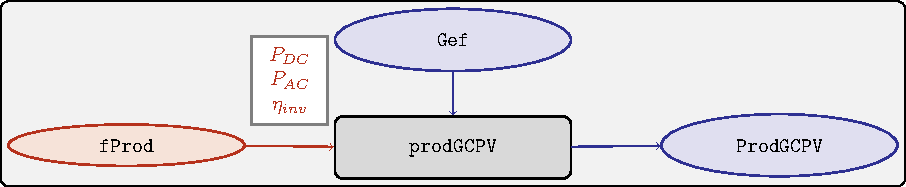
\includegraphics[keepaspectratio,width=\textwidth,height=\textheight]{figuras/prodgcpv.pdf}
\caption{Estimación de la producción eléctrica de un SFCR mediante la función \texttt{prodGCPV}, la cual emplea la función \texttt{fProd} para el computo de la potencia a la entrada (\(P_{DC}\)), a la salida (\(P_{AC}\)) y el rendimiento (\(\eta_{inv}\)) del inversor. \label{fig:prodgcpv}}
\end{figure}
\begin{itemize}
\item \texttt{fProd}: simula el comportamiento de un sistema fotovoltaico conectado a red bajo diferentes condiciones de temperatura e irradiancia. Tiene los siguientes argumentos:
\begin{itemize}
\item \texttt{inclin}: puede ser tanto un objeto de clase \texttt{Gef} como un \texttt{data.frame} (o \texttt{data.table}). Sin embargo, si es un \texttt{data.frame}, debe contener como mínimo una columna para \texttt{Gef} y otra para \texttt{Ta}
\item \texttt{module}: una lista de valores numéricos con la información sobre el módulo fotovoltaico:
\begin{itemize}
\item \texttt{Vocn}: tensión de circuito abierto en STC (\(V_{oc}^*\))(condiciones estandar de médida). Por defecto, tiene un valor de \(57.2V\).
\item \texttt{Iscn}: corriente de cortocircuito en STC (\(I_{sc}^*\)). Por defecto, tiene un valor de \(4.7A\).
\item \texttt{Vmn}: tensión en el punto de máxima potencia en STC (\(I_{MPP}^*\)). Por defecto, tiene un valor de \(46.08V\).
\item \texttt{Imn}: corriente de cortocircuito en STC (\(I_{MPP}^*\)). Por defecto, tiene un valor de \(4.35A\)).
\item \texttt{Ncs}: número de células en serie dentro del módulo. Por defecto, tiene un valor de 96.
\item \texttt{Ncp}: número de células en paralelo dentro del módulo. Por defecto, tiene un valor de 1.
\item \texttt{CoefVT}: coeficiente de disminución de la tensión  de cada célula con la temperatura (\(dV_{oc}/dT_c\)). Por defecto, tiene un valor de \(-0.0023 V/^\circ C\).
\item \texttt{TONC}: temperatura de operación nominal de célula (\(TONC\)). Por defecto, tiene un valor de \(47^\circ C\).
\end{itemize}
\item \texttt{generatos}: lista de valores numéricos con la información sobre el generador:
\begin{itemize}
\item \texttt{Nms}: número de módulos en serie. Por defecto, tiene un valor de 12.
\item \texttt{Nmp}: número de módulos en paralelo. Por defecto, tiene un valor de 11.
\end{itemize}
\item \texttt{inverter}: lista de valores númericos con la información del inversor DC/AC.
\begin{itemize}
\item \texttt{Ki}: coeficientes de la curva de eficiencia del inversor. Se puede presentar en un vector de 3 valores (por defecto, \texttt{c(0.01, 0.025, 0.05)}) o una matriz de 9 valores (si tiene dependencia del voltage).
\item \texttt{Pinv}: potencia nominal del inversor. Por defecto, tiene un valor de \(25000 W\).
\item \texttt{Vmin}: mínima tensión del rango MPP del inversor. Por defecto, tiene un valor de \(420V\).
\item \texttt{Vmax}: máxima tensión del rango MPP del inversor. Por defecto, tiene un valor de \(750V\).
\item \texttt{Gumb}: irradiancia umbral de funcionamienot del inversor. Por defecto, tiene un valor de \(20W/m^2\).
\end{itemize}
\item \texttt{effSys}: una lista de valores numéricos con la información sobre las pérdidas del sistema.
\begin{itemize}
\item \texttt{ModQual}: tolerancia media del set de módulos (\(\%\)). Por defecto, tiene un valor de 3.
\item \texttt{ModDisp}: pérdidas por dispersión en los módulos (\(\%\)). Por defecto, tiene un valor de 2.
\item \texttt{OhmDC}: pérdidas por efecto Joule en el cableado de DC (\(\%\)). Por defecto, tiene un valor de 1.5.
\item \texttt{OhmAC}: pérdidas por efecto Joule en el cableado de AC (\(\%\)). Por defecto, tiene un valor de 1.5.
\item \texttt{MPP}: error promedio del algoritmo de búsqueda del MPP del inversor (\(\%\)). Por defecto, tiene un valor de 1.
\item \texttt{TrafoMT}: pérdidas por el transformador MT (\(\%\)). Por defecto, tiene un valor de 1.
\item \texttt{Disp}: pérdidas por las paradas del sistema (\(\%\)). Por defecto, tiene un valor de 0.5.
\end{itemize}
\end{itemize}
\end{itemize}
\begin{lstlisting}[numbers=left,language=r,label= ,caption= ,captionpos=b]
inclin <- calcGef(lat, dataRad = prom, keep.night = FALSE)
module <- list(Vocn=57.6, Iscn=4.7, Vmn=46.08, Imn=4.35,
               Ncs=96, Ncp=1, CoefVT=0.0023, TONC=47)
generator <- list(Nms=12, Nmp=11)
inverter <- list(Ki=c(0.01, 0.025, 0.05), Pinv=25000,
                 Vmin=420, Vmax=750, Gumb=20)
effSys <- list(ModQual=3, ModDisp=2, OhmDC=1.5, OhmAC=1.5,
               MPP=1, TrafoMT=1, Disp=0.5)
prod <- fProd(inclin = inclin, module = module,
              generator = generator, inverter = inverter,
              effSys = effSys)
show(prod)
\end{lstlisting}

\begin{verbatim}
                   Dates       Tc      Voc       Isc     Vmpp      Impp      Vdc       Idc       Pac
                  <POSc>    <num>    <num>     <num>    <num>     <num>    <num>     <num>     <num>
  1: 2024-01-17 08:00:00 15.27689 716.9624  8.083413 607.4640  7.620135 607.4640  7.620135  3796.209
  2: 2024-01-17 09:00:00 21.43284 700.6516 17.513415 583.9663 16.433741 583.9663 16.433741  8053.912
  3: 2024-01-17 10:00:00 27.23609 685.2753 26.403138 562.0190 24.658263 562.0190 24.658263 11650.920
  4: 2024-01-17 11:00:00 31.48724 674.0114 32.915263 546.0746 30.625265 546.0746 30.625265 14041.629
  5: 2024-01-17 12:00:00 33.33104 669.1261 35.739693 539.1958 33.196772 539.1958 33.196772 15016.481
 ---                                                                                                
141: 2024-12-13 12:00:00 33.94967 667.4869 28.721724 542.4718 26.706186 542.4718 26.706186 12177.570
142: 2024-12-13 13:00:00 32.55186 671.1906 26.580476 547.6944 24.746716 547.6944 24.746716 11395.331
143: 2024-12-13 14:00:00 29.08872 680.3665 21.275466 560.6878 19.868077 560.6878 19.868077  9362.088
144: 2024-12-13 15:00:00 24.29331 693.0724 13.929608 578.8034 13.059814 578.8034 13.059814  6316.091
145: 2024-12-13 16:00:00 19.21305 706.5331  6.147403 598.1441  5.786102 598.1441  5.786102  2784.663
           Pdc      EffI
         <num>     <num>
  1:  4290.940 0.9118076
  2:  8895.974 0.9330800
  3: 12846.437 0.9347232
  4: 15502.477 0.9335163
  5: 16592.492 0.9327431
 ---                    
141: 13429.451 0.9345615
142: 12563.918 0.9347755
143: 10326.335 0.9343983
144:  7007.083 0.9290019
145:  3208.198 0.8945754
\end{verbatim}

Esta función brinda estos datos a la función \texttt{prodGCPV} para que produzca un objeto de clase \texttt{ProdGCPV} como resultado. Esta función tiene como argumentos principales los mismo que \texttt{calcGef}, ya que parte de un objeto tipo \texttt{Gef}, y los argumentos de la función \texttt{fProd}.
\begin{lstlisting}[numbers=left,language=r,label= ,caption= ,captionpos=b]
prodFixed <- prodGCPV(lat, modeTrk = 'fixed', dataRad = prom)
show(prodFixed)
\end{lstlisting}

\begin{verbatim}
Object of class  ProdGCPV 

Source of meteorological information: prom- 

Latitude of source:  37.2 degrees
Latitude for calculations:  37.2 degrees

Monthly avarages:
        Dates       Eac       Edc       Yf
       <char>     <num>     <num>    <num>
 1: Jan. 2024  95.36291 105.62767 3.604158
 2: Feb. 2024 101.50809 112.56166 3.836410
 3: Mar. 2024 110.26945 122.11835 4.167538
 4: Apr. 2024 124.53728 138.29836 4.706778
 5: May. 2024 131.48629 145.91065 4.969410
 6: Jun. 2024 135.89421 150.78725 5.136003
 7: Jul. 2024 134.98501 149.81246 5.101641
 8: Aug. 2024 130.25804 144.39951 4.922989
 9: Sep. 2024 119.91911 132.77648 4.532238
10: Oct. 2024  96.49455 106.99182 3.646928
11: Nov. 2024  90.17737  99.88152 3.408175
12: Dec. 2024  73.89289  81.80967 2.792718

Yearly values:
   Dates     Eac      Edc       Yf
   <int>   <num>    <num>    <num>
1:  2024 41014.8 45473.37 1550.119
-----------------
Mode of tracking:  fixed 
    Inclination:  27.2 
    Orientation:  0 
-----------------
Generator:
    Modules in series:  12 
    Modules in parallel:  11 
    Nominal power (kWp):  26.5
\end{verbatim}

\begin{lstlisting}[numbers=left,language=r,label= ,caption= ,captionpos=b]
prod2x <- prodGCPV(lat, modeTrk = 'two', dataRad = prom)
show(prod2x)
\end{lstlisting}

\begin{verbatim}
Object of class  ProdGCPV 

Source of meteorological information: prom- 

Latitude of source:  37.2 degrees
Latitude for calculations:  37.2 degrees

Monthly avarages:
        Dates      Eac      Edc       Yf
       <char>    <num>    <num>    <num>
 1: Jan. 2024 138.6806 153.2566 5.241314
 2: Feb. 2024 143.4987 158.5247 5.423408
 3: Mar. 2024 151.8477 167.7311 5.738952
 4: Apr. 2024 178.6717 197.4274 6.752741
 5: May. 2024 200.8888 222.0523 7.592419
 6: Jun. 2024 223.9959 247.6903 8.465728
 7: Jul. 2024 214.2749 236.9628 8.098332
 8: Aug. 2024 194.6043 215.1439 7.354902
 9: Sep. 2024 168.9824 186.7349 6.386542
10: Oct. 2024 132.2995 146.0747 5.000145
11: Nov. 2024 128.5783 141.9871 4.859507
12: Dec. 2024 102.9116 113.5613 3.889454

Yearly values:
   Dates      Eac      Edc       Yf
   <int>    <num>    <num>    <num>
1:  2024 60369.04 66710.67 2281.595
-----------------
Mode of tracking:  two 
    Inclination limit: 90 
-----------------
Generator:
    Modules in series:  12 
    Modules in parallel:  11 
    Nominal power (kWp):  26.5
\end{verbatim}

\begin{lstlisting}[numbers=left,language=r,label= ,caption= ,captionpos=b]
prodHoriz <- prodGCPV(lat, modeTrk = 'horiz', dataRad = prom)
show(prodHoriz)
\end{lstlisting}

\begin{verbatim}
Object of class  ProdGCPV 

Source of meteorological information: prom- 

Latitude of source:  37.2 degrees
Latitude for calculations:  37.2 degrees

Monthly avarages:
        Dates       Eac       Edc       Yf
       <char>     <num>     <num>    <num>
 1: Jan. 2024  99.43006 109.66074 3.757873
 2: Feb. 2024 116.24796 128.22238 4.393490
 3: Mar. 2024 137.39485 151.61074 5.192719
 4: Apr. 2024 172.03044 189.97488 6.501741
 5: May. 2024 196.91337 217.61396 7.442169
 6: Jun. 2024 219.15566 242.31468 8.282797
 7: Jul. 2024 210.33644 232.56087 7.949482
 8: Aug. 2024 189.03576 208.87993 7.144442
 9: Sep. 2024 156.22909 172.44519 5.904542
10: Oct. 2024 110.69482 122.11859 4.183614
11: Nov. 2024  94.40734 104.14723 3.568043
12: Dec. 2024  69.94550  77.30532 2.643529

Yearly values:
   Dates      Eac      Edc       Yf
   <int>    <num>    <num>    <num>
1:  2024 54052.14 59697.16 2042.854
-----------------
Mode of tracking:  horiz 
    Inclination limit: 90 
-----------------
Generator:
    Modules in series:  12 
    Modules in parallel:  11 
    Nominal power (kWp):  26.5
\end{verbatim}

\section{Producción eléctrica de un SFB}
\label{sec:orga838fea}
De igual forma que en el apartado anterior, se puede estimar la producción eléctrica de un sistema fotovoltaico de bombeo.

Como se puede ver en la figura \ref{fig:prodpvps}, \texttt{prodPVPS} funciona gracias a la siguiente función:
\begin{figure}[]
\centering
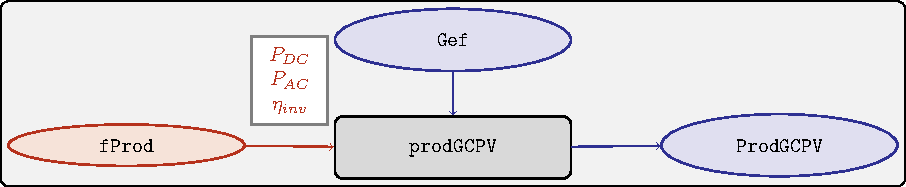
\includegraphics[keepaspectratio,width=\textwidth,height=0.5\textheight]{figuras/prodpvps.pdf}
\caption{Estimación de la producción eléctrica de un SFB mediante la función \texttt{prodPVPS}, la cual emplea la función \texttt{fPump} para el computo del rendimiento de las diferentes parte de una bomba centrífuga alimentada por un convertidor de frecuencia. \label{fig:prodpvps}}
\end{figure}
\begin{itemize}
\item \texttt{fPump}: computa el rendimiento de las diferentes partes de una bomba centrífuga alimentada por un convertidor de frecuencia siguiendo las leyes de afinidad. Tiene solo dos argumentos:
\begin{itemize}
\item \texttt{pump}: lista que contiene los parametros de la bomba que va a ser simulada. Puede ser una fila de \texttt{pumpCoef}:
\begin{lstlisting}[numbers=left,language=r,label= ,caption= ,captionpos=b]
CoefSP8A44 <- pumpCoef[Qn == 8 & stages == 44]
show(CoefSP8A44)
\end{lstlisting}

\begin{verbatim}
      Qn stages  Qmax   Pmn         a         b      c     g     h     i       j     k      l
   <int>  <int> <num> <int>     <num>     <num>  <num> <num> <num> <num>   <num> <num>  <num>
1:     8     44    12  7500 0.1043011 -0.101288 -0.726 -0.24  0.42  0.64 -0.0058 0.095 0.2013
\end{verbatim}

\item \texttt{H}: el salto manometrico total.
\end{itemize}
\begin{lstlisting}[numbers=left,language=r,label= ,caption= ,captionpos=b]
fSP8A44 <- fPump(pump = CoefSP8A44, H = 40)
\end{lstlisting}

Obtiene como resultado los siguientes valores y funciones:
\begin{itemize}
\item \texttt{lim}: rango de valores de la potencia eléctrica de salida.
\begin{lstlisting}[numbers=left,language=r,label= ,caption= ,captionpos=b]
show(fSP8A44$lim)
\end{lstlisting}

\begin{verbatim}
[1]  190.100 4084.218
\end{verbatim}

\item \texttt{fQ}: función que relaciona el caudal con la potencia eléctrica.
\begin{lstlisting}[numbers=left,language=r,label= ,caption= ,captionpos=b]
show(fSP8A44$fQ)
\end{lstlisting}

\begin{verbatim}
function (x, deriv = 0L) 
{
    deriv <- as.integer(deriv)
    if (deriv < 0L || deriv > 3L) 
	stop("'deriv' must be between 0 and 3")
    if (deriv > 0L) {
	z0 <- double(z$n)
	z[c("y", "b", "c")] <- switch(deriv, list(y = z$b, b = 2 * 
	    z$c, c = 3 * z$d), list(y = 2 * z$c, b = 6 * z$d, 
	    c = z0), list(y = 6 * z$d, b = z0, c = z0))
	z[["d"]] <- z0
    }
    res <- .splinefun(x, z)
    if (deriv > 0 && z$method == 2 && any(ind <- x <= z$x[1L])) 
	res[ind] <- ifelse(deriv == 1, z$y[1L], 0)
    res
}
<bytecode: 0x000001418067a708>
<environment: 0x000001417925f6d8>
\end{verbatim}

\item \texttt{fPb}: función que relaciona la potencia del eje de la bomba con la potencia eléctrica del motor.
\begin{lstlisting}[numbers=left,language=r,label= ,caption= ,captionpos=b]
show(fSP8A44$fPb)
\end{lstlisting}

\begin{verbatim}
function (x, deriv = 0L) 
{
    deriv <- as.integer(deriv)
    if (deriv < 0L || deriv > 3L) 
	stop("'deriv' must be between 0 and 3")
    if (deriv > 0L) {
	z0 <- double(z$n)
	z[c("y", "b", "c")] <- switch(deriv, list(y = z$b, b = 2 * 
	    z$c, c = 3 * z$d), list(y = 2 * z$c, b = 6 * z$d, 
	    c = z0), list(y = 6 * z$d, b = z0, c = z0))
	z[["d"]] <- z0
    }
    res <- .splinefun(x, z)
    if (deriv > 0 && z$method == 2 && any(ind <- x <= z$x[1L])) 
	res[ind] <- ifelse(deriv == 1, z$y[1L], 0)
    res
}
<bytecode: 0x000001418067a708>
<environment: 0x0000014179272bd8>
\end{verbatim}

\item \texttt{fPh}: función que relaciona la potencia hidráulica con la potencia eléctrica del motor.
\begin{lstlisting}[numbers=left,language=r,label= ,caption= ,captionpos=b]
show(fSP8A44$fPh)
\end{lstlisting}

\begin{verbatim}
function (x, deriv = 0L) 
{
    deriv <- as.integer(deriv)
    if (deriv < 0L || deriv > 3L) 
	stop("'deriv' must be between 0 and 3")
    if (deriv > 0L) {
	z0 <- double(z$n)
	z[c("y", "b", "c")] <- switch(deriv, list(y = z$b, b = 2 * 
	    z$c, c = 3 * z$d), list(y = 2 * z$c, b = 6 * z$d, 
	    c = z0), list(y = 6 * z$d, b = z0, c = z0))
	z[["d"]] <- z0
    }
    res <- .splinefun(x, z)
    if (deriv > 0 && z$method == 2 && any(ind <- x <= z$x[1L])) 
	res[ind] <- ifelse(deriv == 1, z$y[1L], 0)
    res
}
<bytecode: 0x000001418067a708>
<environment: 0x000001417927d860>
\end{verbatim}

\item \texttt{fFreq}: función que relaciona la frecuencia con la potencia eléctrica del motor.
\begin{lstlisting}[numbers=left,language=r,label= ,caption= ,captionpos=b]
show(fSP8A44$fFreq)
\end{lstlisting}

\begin{verbatim}
function (x, deriv = 0L) 
{
    deriv <- as.integer(deriv)
    if (deriv < 0L || deriv > 3L) 
	stop("'deriv' must be between 0 and 3")
    if (deriv > 0L) {
	z0 <- double(z$n)
	z[c("y", "b", "c")] <- switch(deriv, list(y = z$b, b = 2 * 
	    z$c, c = 3 * z$d), list(y = 2 * z$c, b = 6 * z$d, 
	    c = z0), list(y = 6 * z$d, b = z0, c = z0))
	z[["d"]] <- z0
    }
    res <- .splinefun(x, z)
    if (deriv > 0 && z$method == 2 && any(ind <- x <= z$x[1L])) 
	res[ind] <- ifelse(deriv == 1, z$y[1L], 0)
    res
}
<bytecode: 0x000001418067a708>
<environment: 0x0000014179264158>
\end{verbatim}
\end{itemize}

Se pueden realizar operaciones con este objeto:
\begin{lstlisting}[numbers=left,language=r,label= ,caption= ,captionpos=b]
SP8A44 = with(fSP8A44,{
  Pac = seq(lim[1],lim[2],l=10)
  Pb = fPb(Pac)
  etam = Pb/Pac
  Ph = fPh(Pac)
  etab = Ph/Pb
  f = fFreq(Pac)
  Q = fQ(Pac)
  result = data.table(Q,Pac,Pb,Ph,etam,etab,f)})
show(SP8A44)
\end{lstlisting}

\begin{verbatim}
	     Q       Pac        Pb         Ph      etam      etab        f
	 <num>     <num>     <num>      <num>     <num>     <num>    <num>
 1:  0.3133325  190.1000  124.8346   34.15325 0.6566786 0.2735880 20.47033
 2:  2.0718468  622.7798  429.6728  225.83130 0.6899274 0.5255890 22.33036
 3:  4.0764128 1055.4595  752.8970  444.32900 0.7133358 0.5901591 25.51459
 4:  5.6406747 1488.1393 1087.3665  614.83354 0.7306887 0.5654336 28.73213
 5:  6.9474993 1920.8190 1429.7984  757.27743 0.7443692 0.5296393 31.78514
 6:  8.1028841 2353.4988 1778.0156  883.21437 0.7554776 0.4967416 34.69527
 7:  9.1607296 2786.1786 2130.4683  998.51953 0.7646560 0.4686855 37.49608
 8: 10.1514390 3218.8583 2486.0213 1106.50685 0.7723301 0.4450915 40.21428
 9: 11.0937480 3651.5381 2843.8295 1209.21854 0.7788032 0.4252078 42.86977
10: 12.0000000 4084.2179 3203.2578 1308.00000 0.7843014 0.4083343 45.47737
\end{verbatim}

Está función entrega todos estos resultados a \texttt{prodPVPS} la cual computa los resultados en base a la potencia del generador a simular, y devuleve un objeto de clase \texttt{ProdPVPS}.
\begin{lstlisting}[numbers=left,language=r,label= ,caption= ,captionpos=b]
prodsfb <- prodPVPS(lat, modeTrk = 'fixed', dataRad = prom,
                    pump = CoefSP8A44, H = 40, Pg = SP8A44$Pac[10])
show(prodsfb)
\end{lstlisting}

\begin{verbatim}
Object of class  ProdPVPS 

Source of meteorological information: prom- 

Latitude of source:  37.2 degrees
Latitude for calculations:  37.2 degrees

Monthly avarages:
	Dates      Eac       Qd       Yf
       <char>    <num>    <num>    <num>
 1: Jan. 2024 14.07129 50.46621 3.445284
 2: Feb. 2024 15.43701 54.71213 3.779675
 3: Mar. 2024 17.00102 59.68995 4.162613
 4: Apr. 2024 19.39135 67.24260 4.747874
 5: May. 2024 20.65046 71.34195 5.056160
 6: Jun. 2024 21.63947 74.27359 5.298315
 7: Jul. 2024 22.62915 76.77927 5.540633
 8: Aug. 2024 22.17136 75.07166 5.428546
 9: Sep. 2024 19.61622 67.34348 4.802932
10: Oct. 2024 14.92078 53.24853 3.653277
11: Nov. 2024 13.75298 49.50040 3.367348
12: Dec. 2024 11.21349 40.90244 2.745567

Yearly values:
   Dates      Eac       Qd       Yf
   <int>    <num>    <num>    <num>
1:  2024 6482.059 22589.95 1587.099
-----------------
Mode of tracking:  fixed 
    Inclination:  27.2 
    Orientation:  0 
-----------------
Pump:
    Qn:  8 
    Stages:  44 
Height (m):  40 
Generator (Wp):  4084.218
\end{verbatim}
\end{itemize}

\section{Optimización de distancias}
\label{sec:org8d2402d}
\label{optimizacion-distancias}
Por último, el paquete \texttt{solaR2} contiene una función que permite calcular un conjunto de combinaciones de distancias entre los elementos de un sistema fotovoltaico conectado a red, con el fin de que el usuario posteriormente pueda optar cual es la opción mas rentable en base a los precios del cableado y de la ocupación del terreno.

Esta función es \texttt{optimShd}, la cual en base a una resolución (determinada por el argumento \texttt{res}, el cual, indica el incremento de la secuencia de distancias) obtiene la producción de cada combinación y la plasma en un objeto de clase \texttt{Shade}.
\begin{lstlisting}[numbers=left,language=r,label= ,caption= ,captionpos=b]
struct2x <- list(W = 23.11, L = 9.8, Nrow = 2, Ncol = 3)
dist2x <- list(Lew = c(30, 45), Lns = c(20, 40))
ShdM2x <- optimShd(lat, dataRad = prom, modeTrk = 'two',
                   modeShd = c('area', 'prom'),
                   distances = dist2x, struct = struct2x,
                   res = 5)
show(ShdM2x)
\end{lstlisting}

\begin{verbatim}

  |                                                                                                   
  |                                                                                             |   0%
  |                                                                                                   
  |====                                                                                         |   5%
  |                                                                                                   
  |=========                                                                                    |  10%
  |                                                                                                   
  |=============                                                                                |  14%
  |                                                                                                   
  |==================                                                                           |  19%
  |                                                                                                   
  |======================                                                                       |  24%
  |                                                                                                   
  |===========================                                                                  |  29%
  |                                                                                                   
  |===============================                                                              |  33%
  |                                                                                                   
  |===================================                                                          |  38%
  |                                                                                                   
  |========================================                                                     |  43%
  |                                                                                                   
  |============================================                                                 |  48%
  |                                                                                                   
  |=================================================                                            |  52%
  |                                                                                                   
  |=====================================================                                        |  57%
  |                                                                                                   
  |==========================================================                                   |  62%
  |                                                                                                   
  |==============================================================                               |  67%
  |                                                                                                   
  |==================================================================                           |  71%
  |                                                                                                   
  |=======================================================================                      |  76%
  |                                                                                                   
  |===========================================================================                  |  81%
  |                                                                                                   
  |================================================================================             |  86%
  |                                                                                                   
  |====================================================================================         |  90%
  |                                                                                                   
  |=========================================================================================    |  95%
  |                                                                                                   
  |=============================================================================================| 100%
Object of class  Shade 

Source of meteorological information: prom- 

Latitude of source:  37.2 degrees
Latitude for calculations:  37.2 degrees

Monthly avarages:
Dimensions of structure:
$W
[1] 23.11

$L
[1] 9.8

$Nrow
[1] 2

$Ncol
[1] 3

Shade calculation mode:
[1] "area" "prom"
Productivity without shadows:
Object of class  ProdGCPV 

Source of meteorological information: prom- 

Latitude of source:  37.2 degrees
Latitude for calculations:  37.2 degrees

Monthly avarages:
        Dates      Eac      Edc       Yf
       <char>    <num>    <num>    <num>
 1: Jan. 2024 138.6806 153.2566 5.241314
 2: Feb. 2024 143.4987 158.5247 5.423408
 3: Mar. 2024 151.8477 167.7311 5.738952
 4: Apr. 2024 178.6717 197.4274 6.752741
 5: May. 2024 200.8888 222.0523 7.592419
 6: Jun. 2024 223.9959 247.6903 8.465728
 7: Jul. 2024 214.2749 236.9628 8.098332
 8: Aug. 2024 194.6043 215.1439 7.354902
 9: Sep. 2024 168.9824 186.7349 6.386542
10: Oct. 2024 132.2995 146.0747 5.000145
11: Nov. 2024 128.5783 141.9871 4.859507
12: Dec. 2024 102.9116 113.5613 3.889454

Yearly values:
   Dates      Eac      Edc       Yf
   <int>    <num>    <num>    <num>
1:  2024 60369.04 66710.67 2281.595
-----------------
Mode of tracking:  two 
    Inclination limit: 90 
-----------------
Generator:
    Modules in series:  12 
    Modules in parallel:  11 
    Nominal power (kWp):  26.5 

Summary of results:
      Lew             Lns           H           FS               GRR              Yf      
 Min.   :30.00   Min.   :20   Min.   :0   Min.   :0.01509   Min.   :2.649   Min.   :2104  
 1st Qu.:33.75   1st Qu.:25   1st Qu.:0   1st Qu.:0.02223   1st Qu.:3.946   1st Qu.:2192  
 Median :37.50   Median :30   Median :0   Median :0.02870   Median :4.802   Median :2216  
 Mean   :37.50   Mean   :30   Mean   :0   Mean   :0.03463   Mean   :4.967   Mean   :2203  
 3rd Qu.:41.25   3rd Qu.:35   3rd Qu.:0   3rd Qu.:0.03945   3rd Qu.:6.016   3rd Qu.:2231  
 Max.   :45.00   Max.   :40   Max.   :0   Max.   :0.07769   Max.   :7.948   Max.   :2247
\end{verbatim}

Además, con el argumento \texttt{prog}, podemos indicar si queremos que indique con una barra de progreso el estado de la secuencia.

\begin{lstlisting}[numbers=left,language=r,label= ,caption= ,captionpos=b]
structHoriz = list(L = 4.83)
distHoriz = list(Lew = structHoriz$L * c(2,5))
Shd12HorizBT <- optimShd(lat = lat, dataRad = prom,
                         modeTrk = 'horiz',
                         betaLim = 60,
                         distances = distHoriz, res = 2,
                         struct = structHoriz,
                         modeShd = 'bt',
                         prog = FALSE) #Se quita la barra de progreso
show(Shd12HorizBT)
\end{lstlisting}

\begin{verbatim}
Object of class  Shade 

Source of meteorological information: prom- 

Latitude of source:  37.2 degrees
Latitude for calculations:  37.2 degrees

Monthly avarages:
Dimensions of structure:
$L
[1] 4.83

Shade calculation mode:
[1] "bt"
Productivity without shadows:
Object of class  ProdGCPV 

Source of meteorological information: prom- 

Latitude of source:  37.2 degrees
Latitude for calculations:  37.2 degrees

Monthly avarages:
        Dates       Eac       Edc       Yf
       <char>     <num>     <num>    <num>
 1: Jan. 2024  97.48365 107.53823 3.684309
 2: Feb. 2024 114.31569 126.11751 4.320462
 3: Mar. 2024 135.67629 149.74056 5.127767
 4: Apr. 2024 170.28530 188.06424 6.435785
 5: May. 2024 194.83600 215.33865 7.363657
 6: Jun. 2024 216.37522 239.26256 8.177713
 7: Jul. 2024 208.20413 230.21074 7.868894
 8: Aug. 2024 187.19428 206.84745 7.074845
 9: Sep. 2024 154.37402 170.41035 5.834432
10: Oct. 2024 109.27362 120.57435 4.129901
11: Nov. 2024  92.82584 102.42576 3.508272
12: Dec. 2024  69.13228  76.42401 2.612794

Yearly values:
   Dates      Eac      Edc       Yf
   <int>    <num>    <num>    <num>
1:  2024 53386.77 58969.19 2017.707
-----------------
Mode of tracking:  horiz 
    Inclination limit: 60 
-----------------
Generator:
    Modules in series:  12 
    Modules in parallel:  11 
    Nominal power (kWp):  26.5 

Summary of results:
      Lew              H           FS               GRR              Yf      
 Min.   : 9.66   Min.   :0   Min.   :0.04804   Min.   :2.000   Min.   :1736  
 1st Qu.:13.16   1st Qu.:0   1st Qu.:0.05727   1st Qu.:2.725   1st Qu.:1824  
 Median :16.66   Median :0   Median :0.07295   Median :3.449   Median :1871  
 Mean   :16.66   Mean   :0   Mean   :0.08078   Mean   :3.449   Mean   :1855  
 3rd Qu.:20.16   3rd Qu.:0   3rd Qu.:0.09598   3rd Qu.:4.174   3rd Qu.:1902  
 Max.   :23.66   Max.   :0   Max.   :0.13968   Max.   :4.899   Max.   :1921
\end{verbatim}

\begin{lstlisting}[numbers=left,language=r,label= ,caption= ,captionpos=b]
structFixed = list(L = 5)
distFixed = list(D = structFixed$L*c(1,3))
Shd12Fixed <- optimShd(lat = lat, dataRad = prom,
                       modeTrk = 'fixed',
                       distances = distFixed, res = 2,
                       struct = structFixed,
                       modeShd = 'area',
                       prog = FALSE) #Se quita la barra de progreso
show(Shd12Fixed)
\end{lstlisting}

\begin{verbatim}
Object of class  Shade 

Source of meteorological information: prom- 

Latitude of source:  37.2 degrees
Latitude for calculations:  37.2 degrees

Monthly avarages:
Dimensions of structure:
$L
[1] 5

Shade calculation mode:
[1] "area"
Productivity without shadows:
Object of class  ProdGCPV 

Source of meteorological information: prom- 

Latitude of source:  37.2 degrees
Latitude for calculations:  37.2 degrees

Monthly avarages:
        Dates       Eac       Edc       Yf
       <char>     <num>     <num>    <num>
 1: Jan. 2024  95.36291 105.62767 3.604158
 2: Feb. 2024 101.50809 112.56166 3.836410
 3: Mar. 2024 110.26945 122.11835 4.167538
 4: Apr. 2024 124.53728 138.29836 4.706778
 5: May. 2024 131.48629 145.91065 4.969410
 6: Jun. 2024 135.89421 150.78725 5.136003
 7: Jul. 2024 134.98501 149.81246 5.101641
 8: Aug. 2024 130.25804 144.39951 4.922989
 9: Sep. 2024 119.91911 132.77648 4.532238
10: Oct. 2024  96.49455 106.99182 3.646928
11: Nov. 2024  90.17737  99.88152 3.408175
12: Dec. 2024  73.89289  81.80967 2.792718

Yearly values:
   Dates     Eac      Edc       Yf
   <int>   <num>    <num>    <num>
1:  2024 41014.8 45473.37 1550.119
-----------------
Mode of tracking:  fixed 
    Inclination:  27.2 
    Orientation:  0 
-----------------
Generator:
    Modules in series:  12 
    Modules in parallel:  11 
    Nominal power (kWp):  26.5 

Summary of results:
       D              H           FS                 GRR            Yf      
 Min.   : 5.0   Min.   :0   Min.   :0.0008477   Min.   :1.0   Min.   :1364  
 1st Qu.: 7.5   1st Qu.:0   1st Qu.:0.0015710   1st Qu.:1.5   1st Qu.:1511  
 Median :10.0   Median :0   Median :0.0038992   Median :2.0   Median :1544  
 Mean   :10.0   Mean   :0   Mean   :0.0269608   Mean   :2.0   Mean   :1508  
 3rd Qu.:12.5   3rd Qu.:0   3rd Qu.:0.0252790   3rd Qu.:2.5   3rd Qu.:1548  
 Max.   :15.0   Max.   :0   Max.   :0.1199180   Max.   :3.0   Max.   :1549
\end{verbatim}

\section{Métodos de visualización}
\label{sec:orgf57c308}
\label{sec:metodos-visualizacion}
Una vez creados todos los objetos, para mejorar la visualización de los mismos, \texttt{solaR2} cuanta con una serie de métodos que ayudan a la compresión de los datos obtenidos.

\subsection{Datos meteorológicos}
\label{sec:org3717b46}
La clase \texttt{Meteo} cuenta con un método para \texttt{xyplot}.
\begin{lstlisting}[numbers=left,language=r,label= ,caption= ,captionpos=b]
lat <- 37.2
G0dm = c(2.766,3.491,4.494,5.912,6.989,7.742,
         7.919,7.027,5.369,3.562,2.814,2.179) * 1000;
Ta = c(10, 14.1, 15.6, 17.2, 19.3, 21.2,
       28.4, 29.9, 24.3, 18.2, 17.2, 15.2)
BD <- readG0dm(G0dm = G0dm, Ta = Ta, lat = lat)
show(BD)
\end{lstlisting}

\begin{verbatim}
Object of class  Meteo 

Source of meteorological information: prom- 
Latitude of source:  37.2 degrees

Meteorological Data:
     Dates                 G0d             Ta       
 Min.   :2024-01-17   Min.   :2179   Min.   :10.00  
 1st Qu.:2024-04-07   1st Qu.:3322   1st Qu.:15.50  
 Median :2024-06-29   Median :4932   Median :17.70  
 Mean   :2024-07-01   Mean   :5022   Mean   :19.22  
 3rd Qu.:2024-09-25   3rd Qu.:6998   3rd Qu.:21.98  
 Max.   :2024-12-13   Max.   :7919   Max.   :29.90
\end{verbatim}

\begin{lstlisting}[numbers=left,language=r,label= ,caption= ,captionpos=b]
xyplot(BD)
\end{lstlisting}

\begin{center}
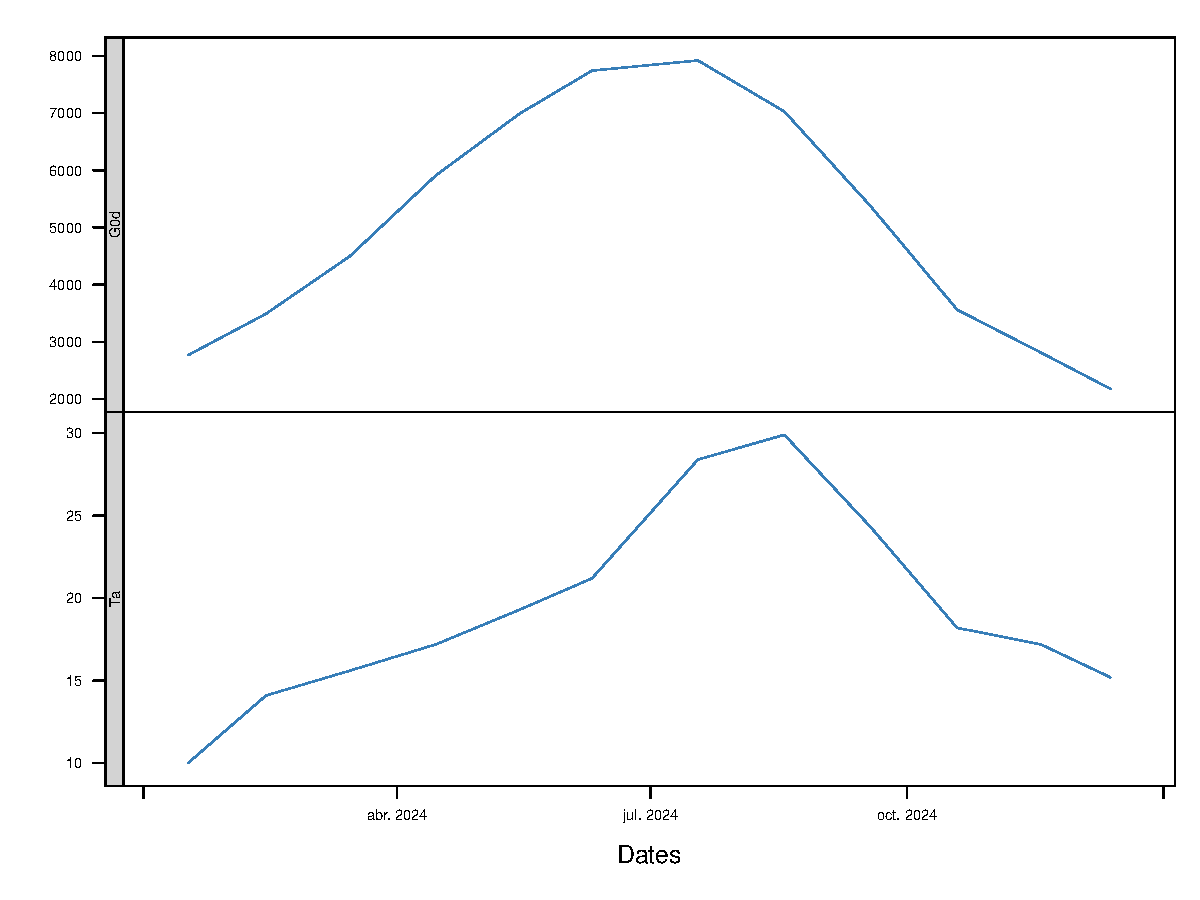
\includegraphics[width=0.8\textwidth]{figuras/codigo-meteo.pdf}
\end{center}

\subsection{Radiación en el plano horizontal}
\label{sec:org3e8045a}
La clase \texttt{G0} cuenta con un método para \texttt{xyplot}.
\begin{lstlisting}[numbers=left,language=r,label= ,caption= ,captionpos=b]
g0 <- calcG0(lat, dataRad = BD)
show(g0)
\end{lstlisting}

\begin{verbatim}
Object of class  G0 

Source of meteorological information: prom- 

Latitude of source:  37.2 degrees
Latitude for calculations:  37.2 degrees

Monthly avarages:
        Dates   G0d      D0d      B0d
       <char> <num>    <num>    <num>
 1: Jan. 2024 2.766 0.941698 1.824302
 2: Feb. 2024 3.491 1.247146 2.243854
 3: Mar. 2024 4.494 1.671763 2.822237
 4: Apr. 2024 5.912 1.931146 3.980854
 5: May. 2024 6.989 2.023364 4.965636
 6: Jun. 2024 7.742 1.889994 5.852006
 7: Jul. 2024 7.919 1.624064 6.294936
 8: Aug. 2024 7.027 1.547591 5.479409
 9: Sep. 2024 5.369 1.540708 3.828292
10: Oct. 2024 3.562 1.374513 2.187487
11: Nov. 2024 2.814 1.006959 1.807041
12: Dec. 2024 2.179 0.926737 1.252263

Yearly values:
   Dates      G0d      D0d      B0d
   <int>    <num>    <num>    <num>
1:  2024 1839.365 540.6331 1298.732
\end{verbatim}

\begin{lstlisting}[numbers=left,language=r,label= ,caption= ,captionpos=b]
xyplot(g0)
\end{lstlisting}

\begin{center}
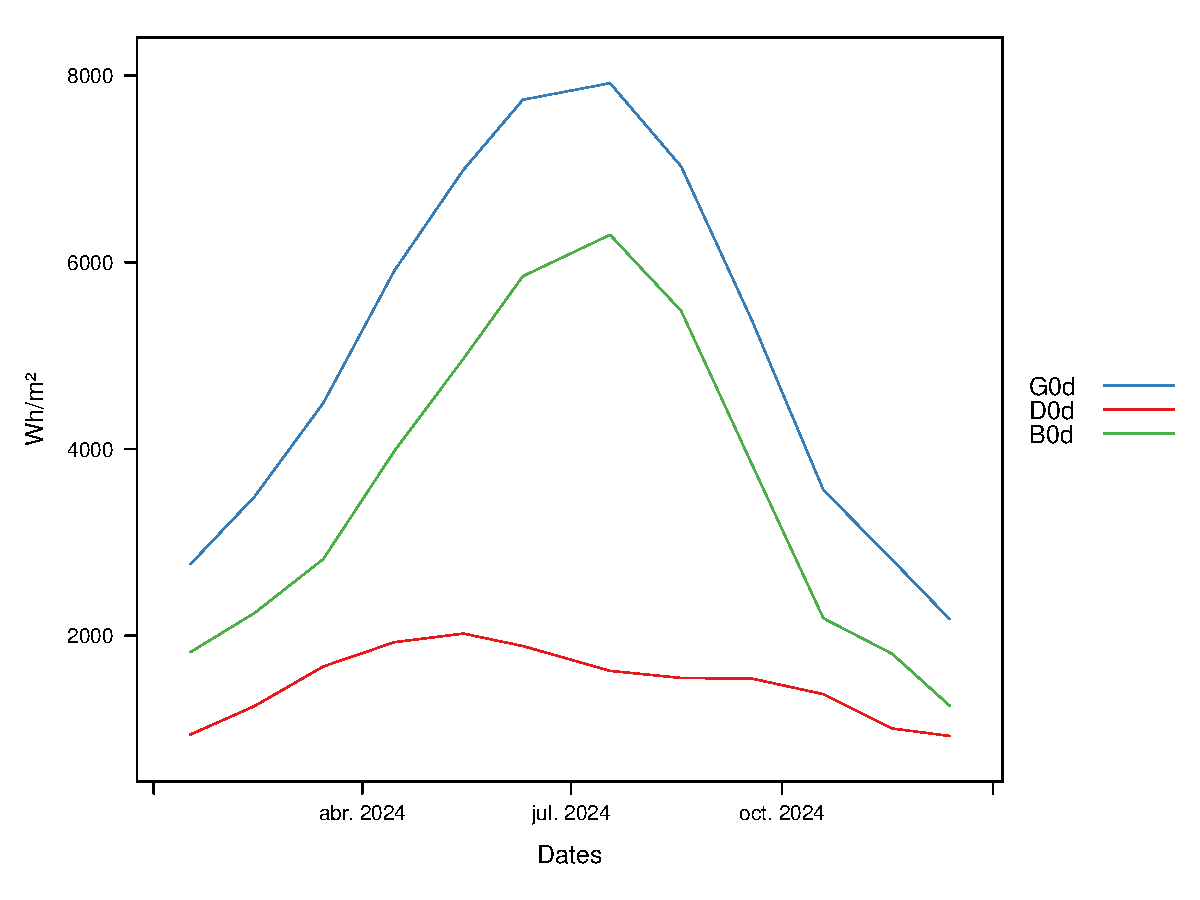
\includegraphics[width=0.8\textwidth]{figuras/codigo-g0.pdf}
\end{center}

Y con un método para \texttt{compare}.
\begin{lstlisting}[numbers=left,language=r,label= ,caption= ,captionpos=b]
g02 <- calcG0(lat, dataRad = list(G0dm = G0dm*0.95, Ta = Ta))
compare(g0, g02)
\end{lstlisting}

\begin{center}
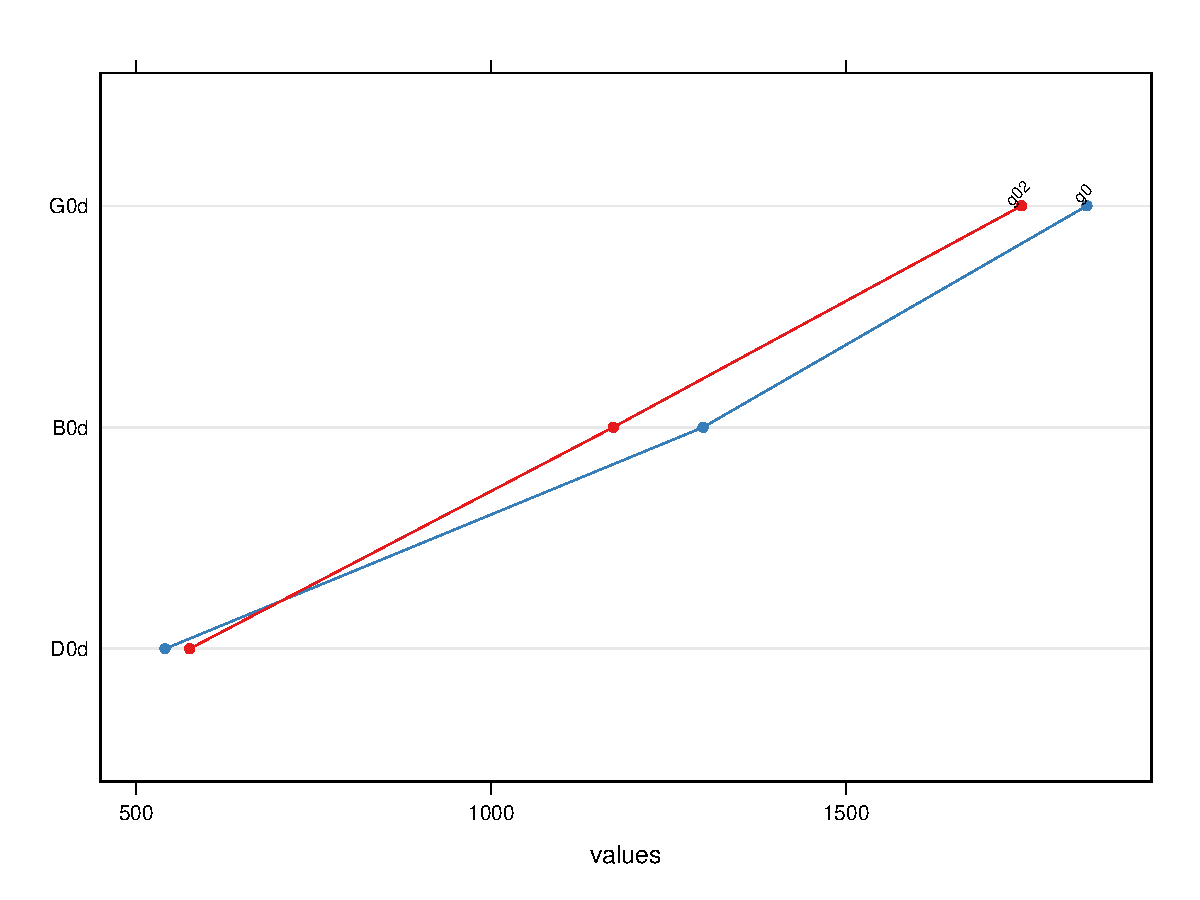
\includegraphics[width=0.8\textwidth]{figuras/codigo-g02.pdf}
\end{center}

\subsection{Radiación efectiva en el plano del generador}
\label{sec:orga7e5c37}
La clase \texttt{Gef} cuenta con un método para \texttt{xyplot}.
\begin{lstlisting}[numbers=left,language=r,label= ,caption= ,captionpos=b]
gef <- calcGef(lat, dataRad = BD)
show(gef)
\end{lstlisting}

\begin{verbatim}
Object of class  Gef 

Source of meteorological information: prom- 

Latitude of source:  37.2 degrees
Latitude for calculations:  37.2 degrees

Monthly avarages:
        Dates       Bod       Bnd       Gd       Dd       Bd     Gefd     Defd     Befd
       <char>     <num>     <num>    <num>    <num>    <num>    <num>    <num>    <num>
 1: Jan. 2024  8.724907  4.924221 4.489744 1.200992 3.258164 4.220907 1.119517 3.080392
 2: Feb. 2024  9.592013  5.034287 4.919206 1.451954 3.428647 4.628492 1.352529 3.249460
 3: Mar. 2024 10.281308  5.163713 5.413543 1.779951 3.583896 5.101556 1.657369 3.410070
 4: Apr. 2024 10.527227  6.408617 6.282631 1.936897 4.280357 5.918787 1.803811 4.070094
 5: May. 2024 10.431853  7.617499 6.784202 1.937331 4.769584 6.371295 1.802060 4.516177
 6: Jun. 2024 10.291163  9.102430 7.173475 1.762326 5.325535 6.725684 1.639192 5.027718
 7: Jul. 2024 10.305302 10.037233 7.511733 1.533887 5.890275 7.058263 1.430322 5.567823
 8: Aug. 2024 10.394682  8.640959 7.295543 1.545089 5.672747 6.879777 1.443952 5.382478
 9: Sep. 2024 10.233884  6.698488 6.335591 1.647975 4.628244 5.982520 1.539552 4.402209
10: Oct. 2024  9.659077  4.546024 4.746760 1.538325 3.169044 4.470026 1.432213 3.010771
11: Nov. 2024  8.798687  4.638289 4.393712 1.244217 3.118376 4.134590 1.159756 2.953471
12: Dec. 2024  8.176298  3.439788 3.478125 1.128381 2.325648 3.274677 1.050626 2.207509

Yearly values:
   Dates      Bod      Bnd       Gd       Dd       Bd     Gefd     Defd     Befd
   <int>    <num>    <num>    <num>    <num>    <num>    <num>    <num>    <num>
1:  2024 3580.873 2326.882 2099.528 570.4317 1508.756 1975.745 531.5105 1430.271
-----------------
Mode of tracking:  fixed 
    Inclination:  27.2 
    Orientation:  0
\end{verbatim}

\begin{lstlisting}[numbers=left,language=r,label= ,caption= ,captionpos=b]
xyplot(gef)
\end{lstlisting}

\begin{center}
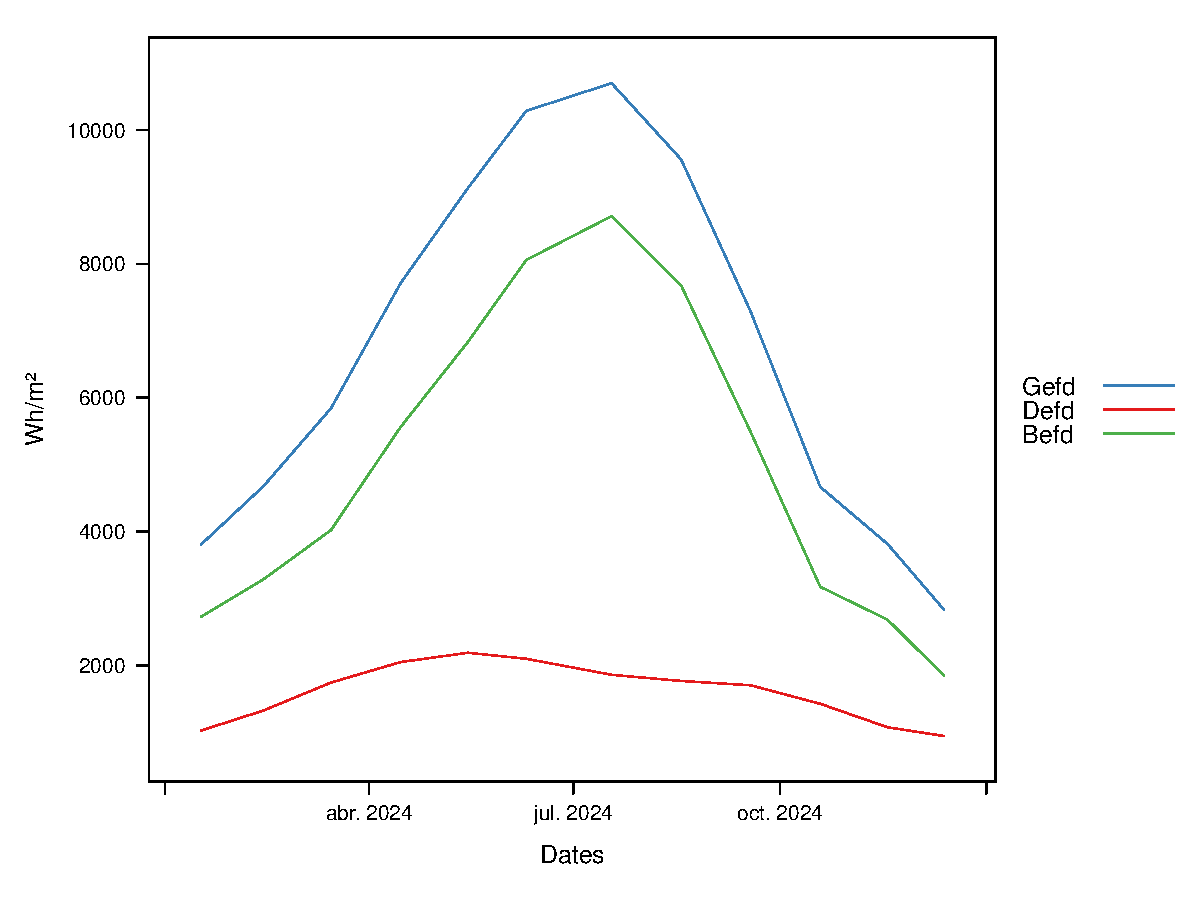
\includegraphics[width=0.8\textwidth]{figuras/codigo-gef.pdf}
\end{center}

Y con un método para \texttt{compare}.
\begin{lstlisting}[numbers=left,language=r,label= ,caption= ,captionpos=b]
gef2x <- calcGef(lat, modeTrk = 'two', dataRad = BD)
gefhoriz <- calcGef(lat, modeTrk = 'horiz', dataRad = BD)
compare(gef, gef2x, gefhoriz)
\end{lstlisting}

\begin{center}
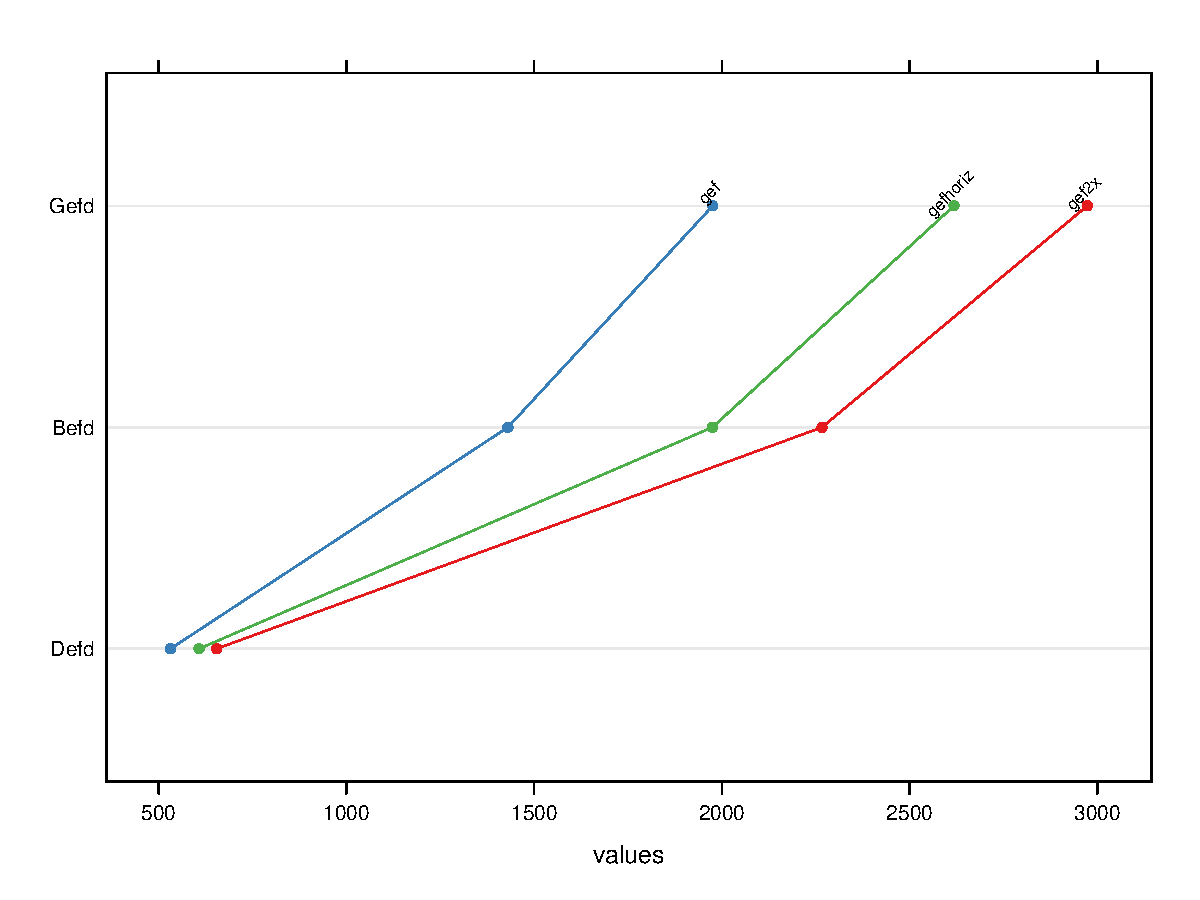
\includegraphics[width=0.8\textwidth]{figuras/codigo-gef2.pdf}
\end{center}


\subsection{Producción eléctrica de un SFCR}
\label{sec:orgdcd6f78}
La clase \texttt{ProdGCPV} cuenta con un método para \texttt{xyplot}.
\begin{lstlisting}[numbers=left,language=r,label= ,caption= ,captionpos=b]
prodFixed <- prodGCPV(lat, modeTrk = 'fixed', dataRad = BD)
show(prodFixed)
\end{lstlisting}

\begin{verbatim}
Object of class  ProdGCPV 

Source of meteorological information: prom- 

Latitude of source:  37.2 degrees
Latitude for calculations:  37.2 degrees

Monthly avarages:
        Dates       Eac       Edc       Yf
       <char>     <num>     <num>    <num>
 1: Jan. 2024  95.36291 105.62767 3.604158
 2: Feb. 2024 101.50809 112.56166 3.836410
 3: Mar. 2024 110.26945 122.11835 4.167538
 4: Apr. 2024 124.53728 138.29836 4.706778
 5: May. 2024 131.48629 145.91065 4.969410
 6: Jun. 2024 135.89421 150.78725 5.136003
 7: Jul. 2024 134.98501 149.81246 5.101641
 8: Aug. 2024 130.25804 144.39951 4.922989
 9: Sep. 2024 119.91911 132.77648 4.532238
10: Oct. 2024  96.49455 106.99182 3.646928
11: Nov. 2024  90.17737  99.88152 3.408175
12: Dec. 2024  73.89289  81.80967 2.792718

Yearly values:
   Dates     Eac      Edc       Yf
   <int>   <num>    <num>    <num>
1:  2024 41014.8 45473.37 1550.119
-----------------
Mode of tracking:  fixed 
    Inclination:  27.2 
    Orientation:  0 
-----------------
Generator:
    Modules in series:  12 
    Modules in parallel:  11 
    Nominal power (kWp):  26.5
\end{verbatim}

\begin{lstlisting}[numbers=left,language=r,label= ,caption= ,captionpos=b]
xyplot(prodFixed)
\end{lstlisting}

\begin{center}
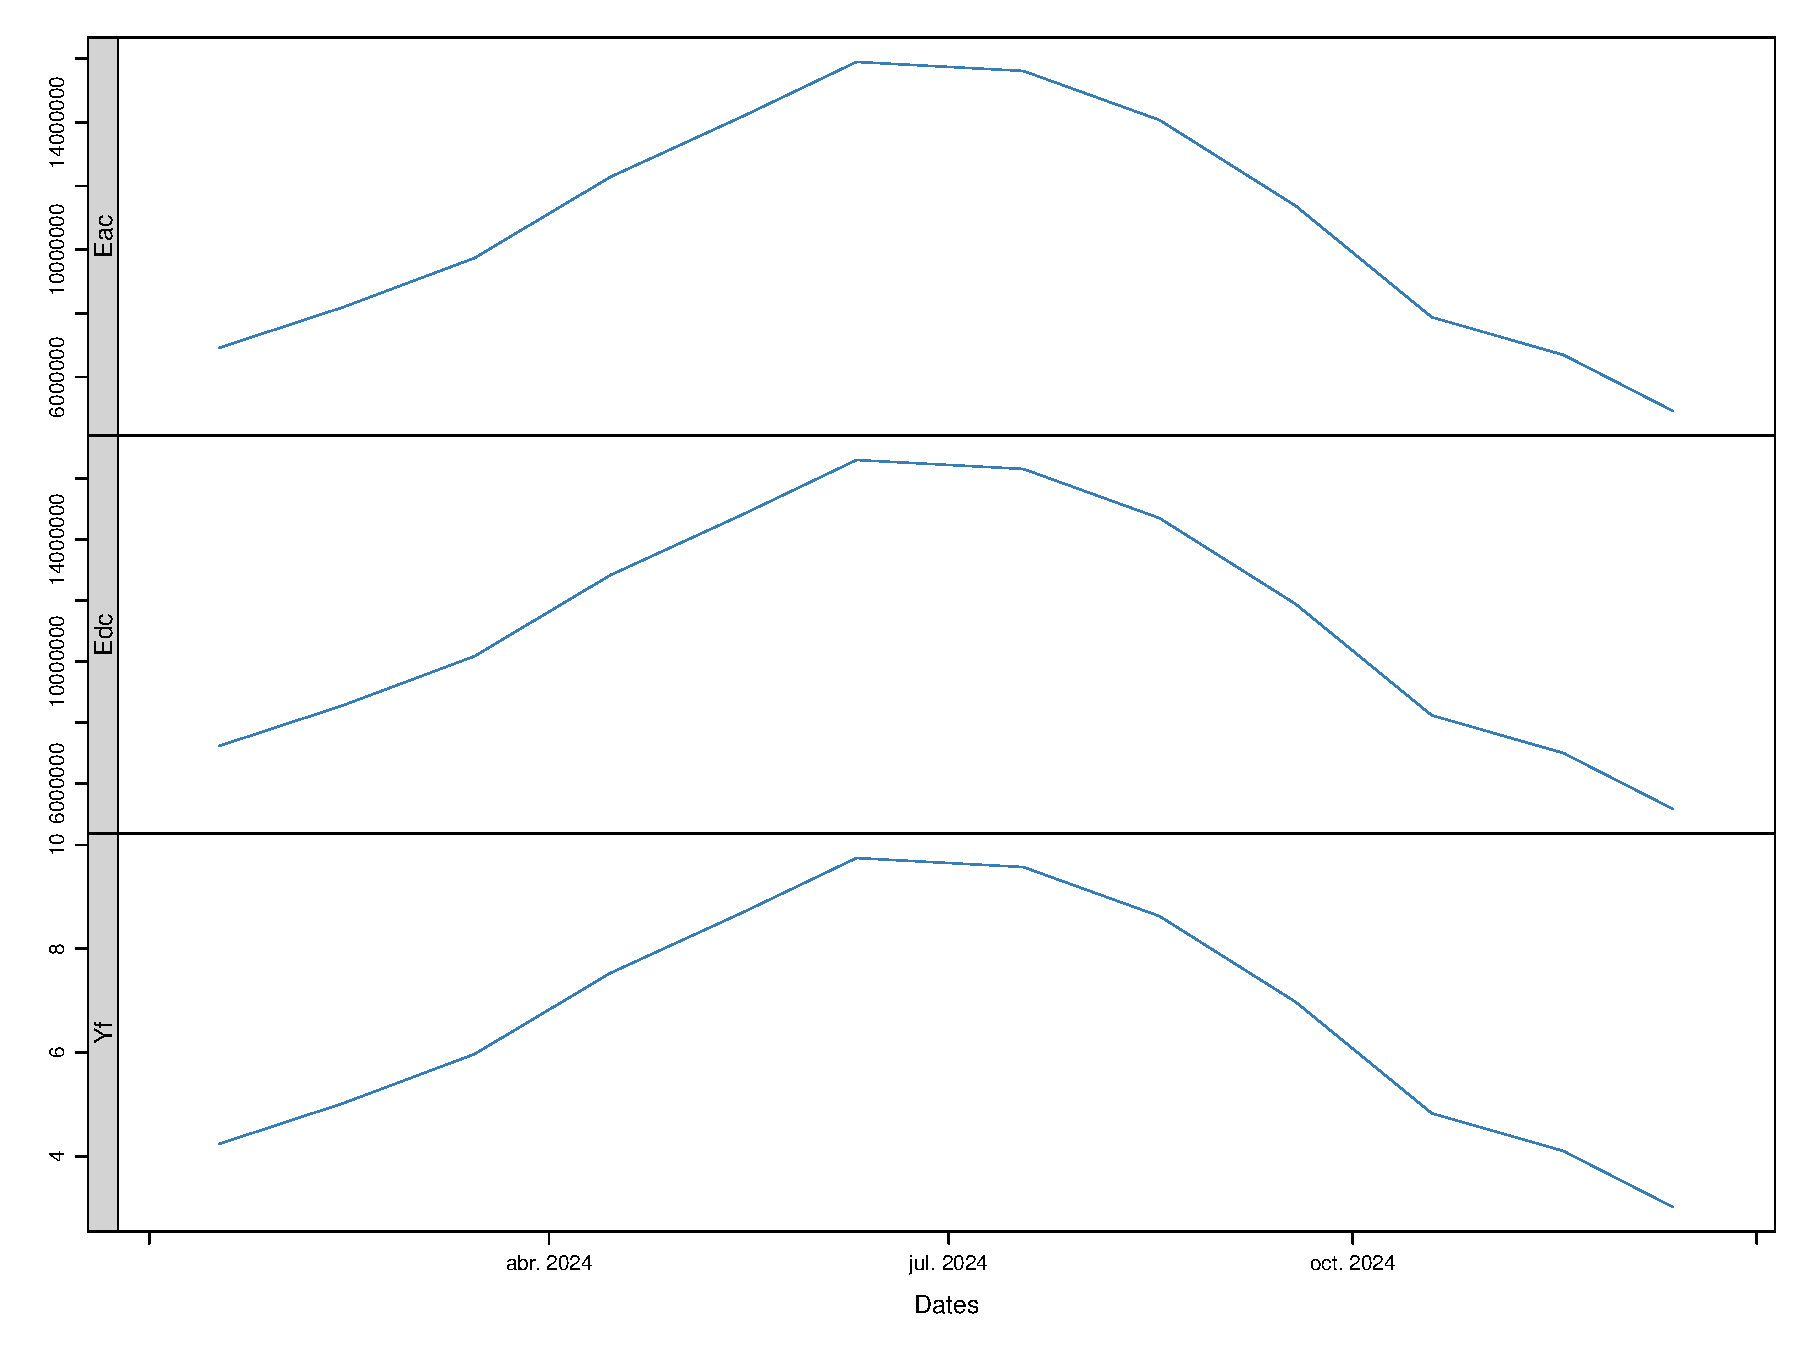
\includegraphics[width=0.8\textwidth]{figuras/codigo-prodgcpv.pdf}
\end{center}

Un método para \texttt{compare}.
\begin{lstlisting}[numbers=left,language=r,label= ,caption= ,captionpos=b]
prod2x <- prodGCPV(lat, modeTrk = 'two', dataRad = BD)
prodHoriz <- prodGCPV(lat, modeTrk = 'horiz', dataRad = BD)
compare(prodFixed, prod2x, prodHoriz)
\end{lstlisting}

\begin{center}
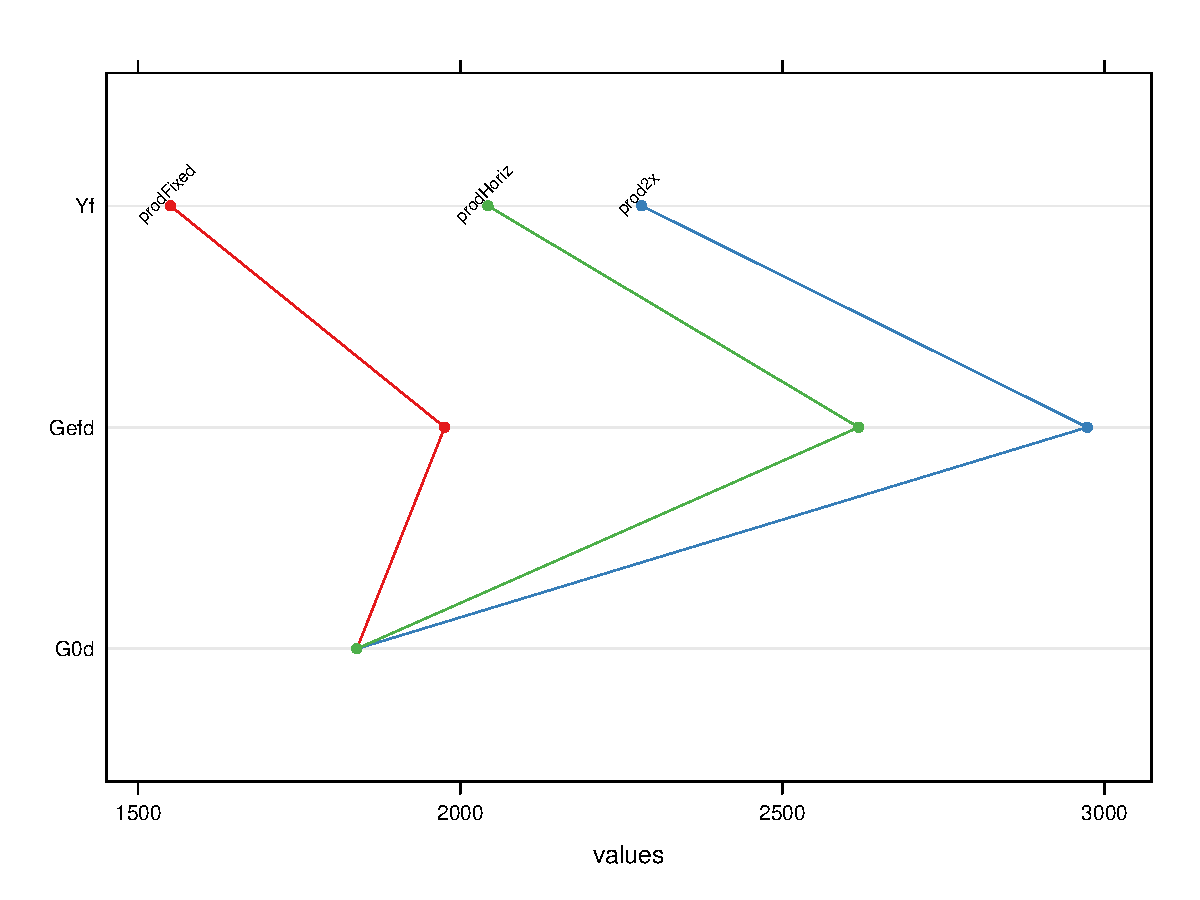
\includegraphics[width=0.8\textwidth]{figuras/codigo-prodgcpv2.pdf}
\end{center}

Y un método para \texttt{compareLosses}.
\begin{lstlisting}[numbers=left,language=r,label= ,caption= ,captionpos=b]
compareLosses(prodFixed, prod2x, prodHoriz)
\end{lstlisting}

\begin{center}
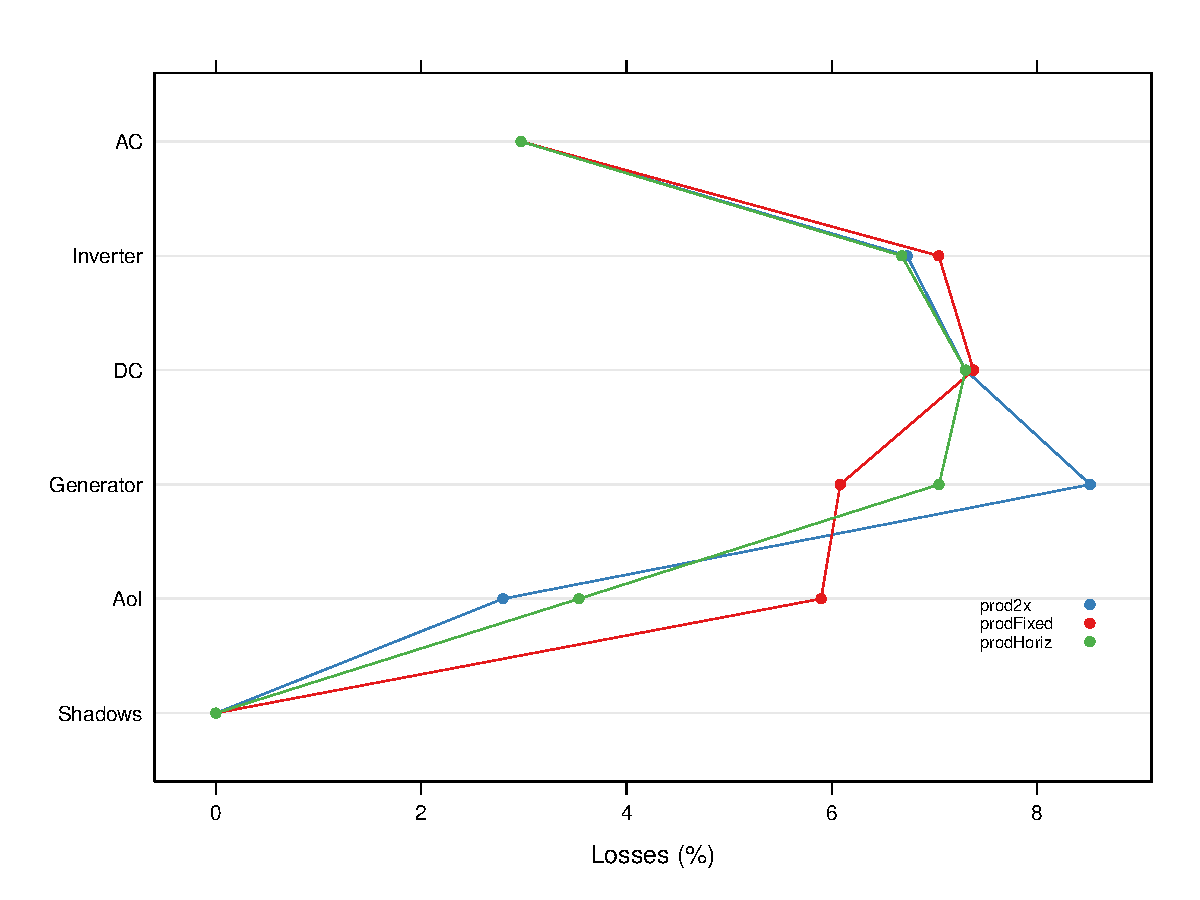
\includegraphics[width=0.8\textwidth]{figuras/codigo-prodgcpv3.pdf}
\end{center}

\subsection{Producción electrica de un SFB}
\label{sec:org60ae102}
La clase \texttt{ProdPVPS} cuenta con un método para \texttt{xyplot}.
\begin{lstlisting}[numbers=left,language=r,label= ,caption= ,captionpos=b]
pump <- prodPVPS(lat, dataRad = BD, pump = CoefSP8A44, H = 40, Pg = 5000)
show(pump)
\end{lstlisting}

\begin{verbatim}
Object of class  ProdPVPS 

Source of meteorological information: prom- 

Latitude of source:  37.2 degrees
Latitude for calculations:  37.2 degrees

Monthly avarages:
        Dates      Eac       Qd       Yf
       <char>    <num>    <num>    <num>
 1: Jan. 2024 17.22642 59.71506 3.445284
 2: Feb. 2024 18.89837 64.60949 3.779675
 3: Mar. 2024 20.81307 70.36542 4.162613
 4: Apr. 2024 23.73937 79.08382 4.747874
 5: May. 2024 25.28080 83.74003 5.056160
 6: Jun. 2024 26.49158 87.02474 5.298315
 7: Jul. 2024 27.70317 89.81648 5.540633
 8: Aug. 2024 27.14273 87.89528 5.428546
 9: Sep. 2024 24.01466 79.04010 4.802932
10: Oct. 2024 18.26638 63.00860 3.653277
11: Nov. 2024 17.06794 59.03182 3.413588
12: Dec. 2024 13.72784 48.99686 2.745567

Yearly values:
   Dates      Eac       Qd       Yf
   <int>    <num>    <num>    <num>
1:  2024 7942.432 26608.76 1588.486
-----------------
Mode of tracking:  fixed 
    Inclination:  27.2 
    Orientation:  0 
-----------------
Pump:
    Qn:  8 
    Stages:  44 
Height (m):  40 
Generator (Wp):  5000
\end{verbatim}

\begin{lstlisting}[numbers=left,language=r,label= ,caption= ,captionpos=b]
xyplot(pump)
\end{lstlisting}

\begin{center}
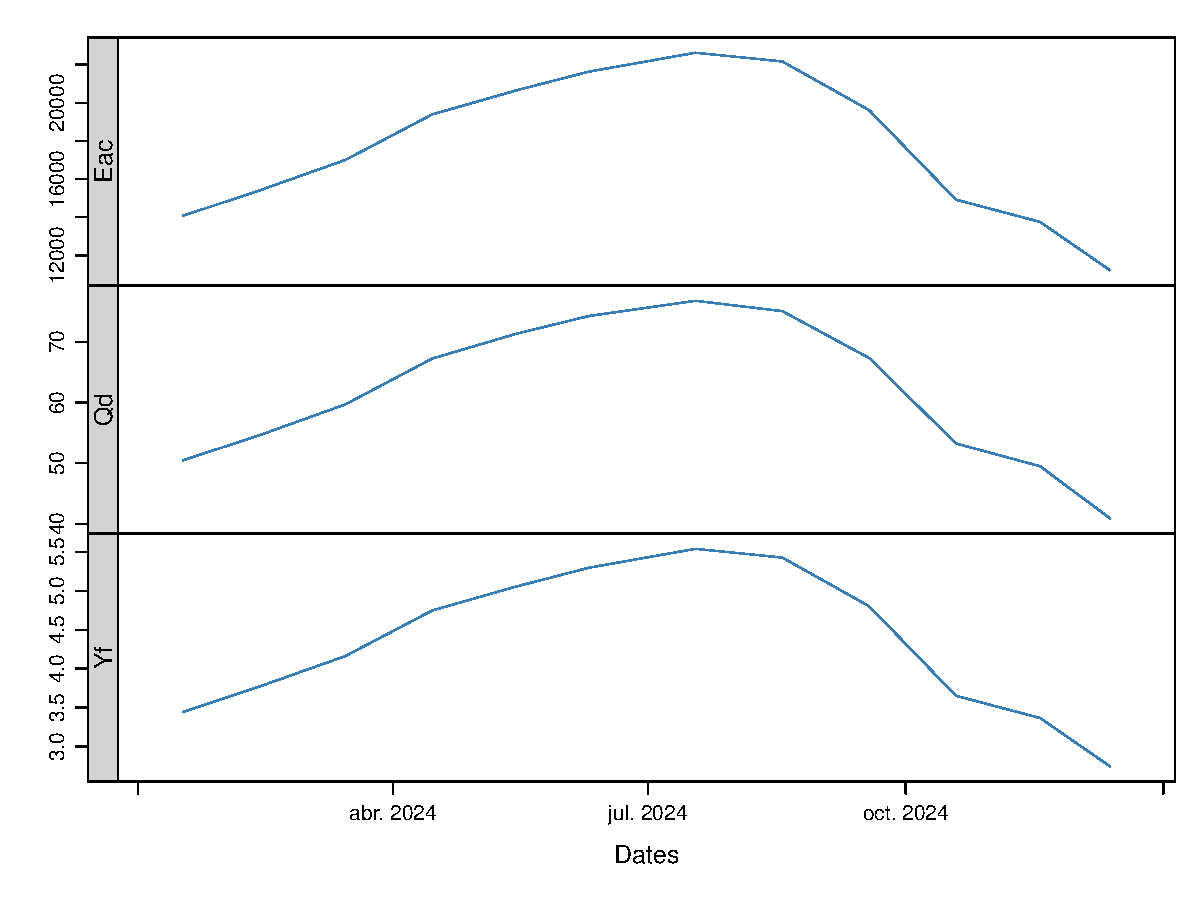
\includegraphics[width=.9\linewidth]{figuras/codigo-prodpvps.pdf}
\end{center}

\subsection{Optimización de distancias}
\label{sec:orge297e7d}
La clase \texttt{Shade} cuenta con un método para \texttt{shadeplot}.
\begin{lstlisting}[numbers=left,language=r,label= ,caption= ,captionpos=b]
struct2x = list(W = 23.11, L = 9.8, Nrow = 2, Ncol = 3)
dist2x = list(Lew = c(30, 45),Lns = c(20, 40))
ShdM2x <- optimShd(lat = lat, dataRad = prom, modeTrk = 'two',
                    modeShd = c('area','prom'),
                   distances = dist2x, struct = struct2x,
                   res = 5, prog = FALSE)
show(ShdM2x)
\end{lstlisting}

\begin{verbatim}
Object of class  Shade 

Source of meteorological information: prom- 

Latitude of source:  37.2 degrees
Latitude for calculations:  37.2 degrees

Monthly avarages:
Dimensions of structure:
$W
[1] 23.11

$L
[1] 9.8

$Nrow
[1] 2

$Ncol
[1] 3

Shade calculation mode:
[1] "area" "prom"
Productivity without shadows:
Object of class  ProdGCPV 

Source of meteorological information: prom- 

Latitude of source:  37.2 degrees
Latitude for calculations:  37.2 degrees

Monthly avarages:
        Dates      Eac      Edc       Yf
       <char>    <num>    <num>    <num>
 1: Jan. 2024 138.6806 153.2566 5.241314
 2: Feb. 2024 143.4987 158.5247 5.423408
 3: Mar. 2024 151.8477 167.7311 5.738952
 4: Apr. 2024 178.6717 197.4274 6.752741
 5: May. 2024 200.8888 222.0523 7.592419
 6: Jun. 2024 223.9959 247.6903 8.465728
 7: Jul. 2024 214.2749 236.9628 8.098332
 8: Aug. 2024 194.6043 215.1439 7.354902
 9: Sep. 2024 168.9824 186.7349 6.386542
10: Oct. 2024 132.2995 146.0747 5.000145
11: Nov. 2024 128.5783 141.9871 4.859507
12: Dec. 2024 102.9116 113.5613 3.889454

Yearly values:
   Dates      Eac      Edc       Yf
   <int>    <num>    <num>    <num>
1:  2024 60369.04 66710.67 2281.595
-----------------
Mode of tracking:  two 
    Inclination limit: 90 
-----------------
Generator:
    Modules in series:  12 
    Modules in parallel:  11 
    Nominal power (kWp):  26.5 

Summary of results:
      Lew             Lns           H           FS               GRR              Yf      
 Min.   :30.00   Min.   :20   Min.   :0   Min.   :0.01509   Min.   :2.649   Min.   :2104  
 1st Qu.:33.75   1st Qu.:25   1st Qu.:0   1st Qu.:0.02223   1st Qu.:3.946   1st Qu.:2192  
 Median :37.50   Median :30   Median :0   Median :0.02870   Median :4.802   Median :2216  
 Mean   :37.50   Mean   :30   Mean   :0   Mean   :0.03463   Mean   :4.967   Mean   :2203  
 3rd Qu.:41.25   3rd Qu.:35   3rd Qu.:0   3rd Qu.:0.03945   3rd Qu.:6.016   3rd Qu.:2231  
 Max.   :45.00   Max.   :40   Max.   :0   Max.   :0.07769   Max.   :7.948   Max.   :2247
\end{verbatim}

\begin{lstlisting}[numbers=left,language=r,label= ,caption= ,captionpos=b]
shadeplot(ShdM2x)
\end{lstlisting}

\begin{center}
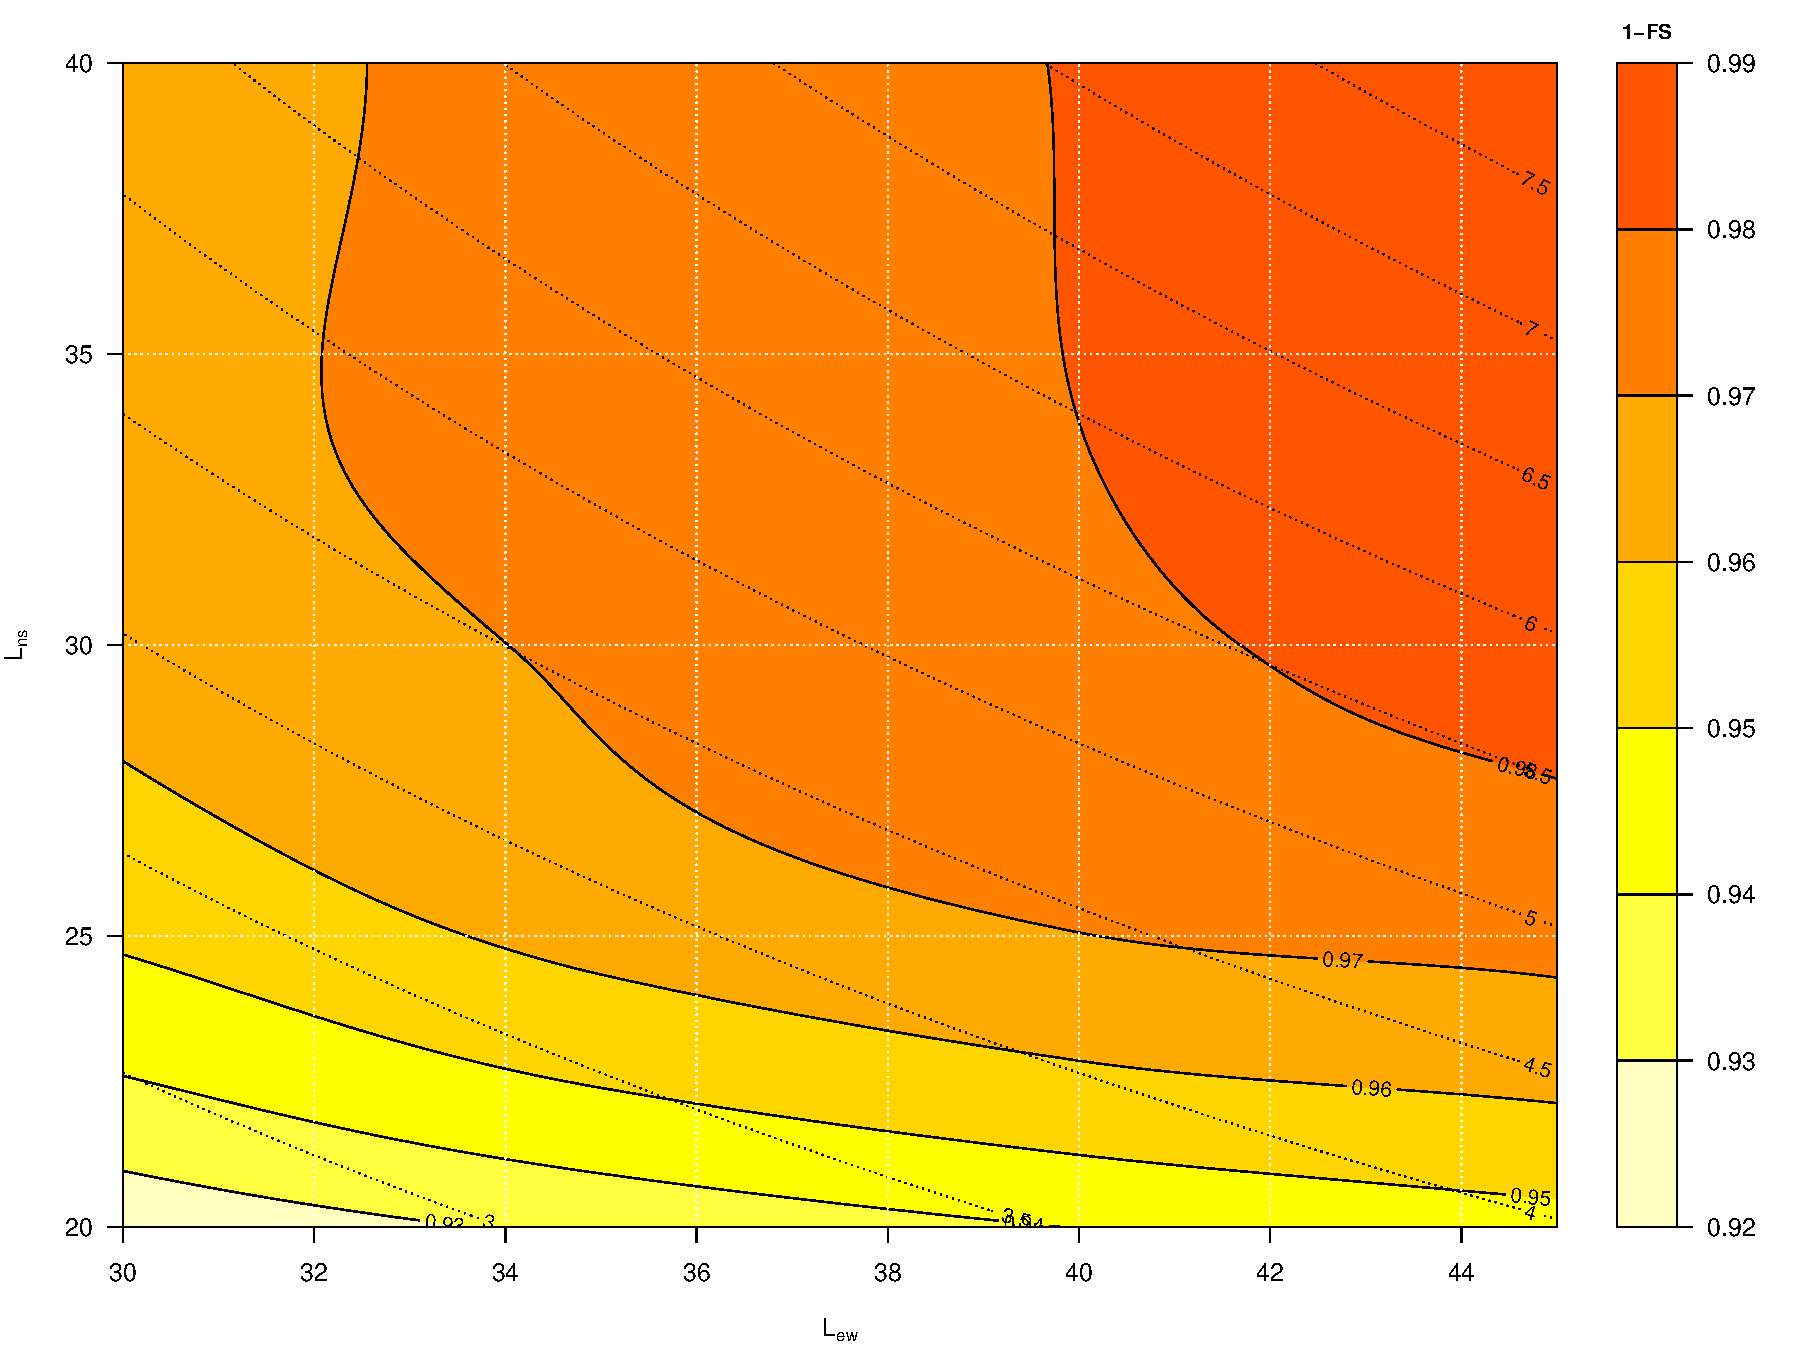
\includegraphics[width=0.8\textwidth]{figuras/codigo-optimshd.pdf}
\end{center}


\chapter{Ejemplo práctico de aplicación}
\label{chap:ejemplo-practico-aplicacion}
Como demostración se va a realizar un caso práctico\ldots{}

\section{\texttt{solaR}}
\label{sec:org3a43d49}

\ldots{}


\section{\texttt{PVsyst}}
\label{sec:orgaff593d}

\ldots{}


\section{\texttt{solaR}}
\label{sec:orgf42178d}

\ldots{}

\section{Comparación entre los tres}
\label{sec:org2ce52e4}


\appendix

\chapter{Manual de referencia de \texttt{solaR2}}
\label{chap:manual}
En este apéndice se incluye el manual de referencia del paquete solaR2. Este manual se genera en base a los archivos de documentación (\texttt{.Rd}) propios de un paquete de R, y en el cual se recoge la información de todas las funciones, objetos y set de datos que contiene el paquete.

Se distribuye siguiendo la siguiente nomenclatura:
\begin{itemize}
\item \textbf{Constructores}: se trata de funciones que devuelven un objeto de una clase propia del paquete. Como identificador, se añade la letra \textbf{A} antes del nombre.
\item \textbf{Clases}: la definición de las clases de los objetos definidos por este paquete. Como identificador, se añade la letra \textbf{B} antes del nombre.
\item \textbf{Utilidades}: funciones que sirven de apoyo a los cálculos de las funciones constructoras. Como identificador, se añade la letra \textbf{C} antes del nombre.
\item \textbf{Métodos}: métodos para los objetos definidos en el paquete. Como identificador, se añade la letra \textbf{D} antes del nombre.
\end{itemize}
\includepdf[pages=-, pagecommand={}]{../../solaR2.Rcheck/solaR2-manual.pdf}


\backmatter

\cleardoublepage

\printbibliography
\end{document}
